\chapter{Establishment of laboratory methods and analytical tools to assess genome-wide chromatin accessibility in clinical samples}
\chaptermark{Establishment of methods to assess genome-wide chromatin accessibility}
\label{ch:Results1}


%%%%%%%%%%%%%%%%%%%%%%%%%%%%%%%%%%%%%%%%%%%%%%%%%%
\section{Introduction}
\subsection*{Previous and current methods to identify the accessible genome in cells and tissues}

\subsection*{Implementation of ATAC-seq to define the chromatin landscape}

\subsection*{Technical limitations and recent advances in optimisation}
https://www.ncbi.nlm.nih.gov/pmc/articles/PMC4473780/

Talk about ATAC being more variable, a native chromatin accessibility assessment without cross-linking. Role of transposase ability in accessing the chromatin, debri and DNA from dead cells adding noise

Paper to justify peak calling: A comparison of peak callers used for DNase-Seq data.

New ATAC but also explanations of the limitations: Characterization of chromatin accessibility with a transposome hypersensitive sites sequencing (THS-seq) assay

\subsection*{Challenges of working with clinical samples}

%%%%%%%%%%%%%%%%%%%%%%%%%%%%%%%%%%%%%%%%%%%%%%%%%%
\section{Results}
%

\subsection{Establishment of an ATAC-seq data analysis pipeline based on current knowledge}
When the first ATAC-seq publication \parencite{Buenrostro2013} appeared, there were not well established protocols for the complete processing of the data. Since then, several publications have used ATAC-seq and modifications of this protocol together with a wide range of data analysis strategies to answer different biological questions (Table \ref{tab:ATAC_comparative_methods}).
There are several limiting aspects in the process of analysing ATAC-seq data, including QC assessment, peak calling/filtering and differential analysis of chromatin accessibility regions between groups. Using the current knowledge in the field as well as on my own analysis, I agreed on the most appropriate criteria and parameters to implement in our in-house pipeline. For this purpose, I used ATAC data generated with the first protocol \parencite{Buenrostro2013} in paired CD14$^+$ monocytes and CD4$^+$ total T cells from the same three healthy individuals, all of them downsamples to 30 million of reads, in order to facilitate the comparison across all of them.


%
\begin{landscape}
\begin{center}
\begin{longtable}[ht]{p{.20\textheight} p{.40\textheight} p{.40\textheight} p{.40\textheight}}
\caption[Summary table of ATAC-seq methodology analysis for peak calling, filtering and differential analysis.]{\textbf{.}}
\label{tab:ATAC_comparative_methods} \\
\toprule
\textbf{Publication} & \textbf{Peak calling and filtering} & \textbf{Master list} & \textbf{Differential analysis} \\
\midrule
\midrule
Corces \textit{et al.}, 2016 & MACS2 (-nomodel), peak summit extension $+/-$250bp, rank summits by pval & Maximally significant non-overlapping peaks. & Quantile normalisation and unsupervised hierarchical clustering. \\
&&&&
ENCODE  & MACS2 -nomodel, pairwise IDR analysis, filtering IDR$<$10\% & Choosing longest pairwise IDR filtered list or only peaks present in the two samples pseudoreplicates. & NA \\
&&&&              
Turner \textit{et al.}, 2018 	& MACS2 (-nomodel --q 0.01) & Merging all filtered called peaks from the different cell types. & \texti{De novo}:DiffReps with fragment size 50bp. \\                             
&&&&																																										
Alasoo \textit{et al.}, 2018 & MACS2 (-nomodel -shift -25 -extsize 50 --q 0.01 &	Union of peaks from all conditions present in at least in three samples of the same condition. & Peak based: TMM normalisation and lima voom (FDR$<$0.01).\\ 
&&&&
Qu \textit{et al.}, 2017 & ZINBA PP$>$0.99. & Merging of filtered peaks from each individual sample. & Quantile normalisation and peak based in house Pearson correlation method. \\							
&&&&
Rendeiro \textit{et al.} 2016 & MACS2 (-nomodel -extsize 147)	& Merge of peaks from all samples in an iterative process including permutations & Peak based: quantile normalisation and Fisher exact text (FDR$<$0.05). \\
&&&&
Scharer\textit{et al.} 2016 & HOMER (-style dnase) & Merge of all overlapping peaks between all samples using HOMER mergePeaks & Peak based: TMM normalisation and edgeR package (FDR$<$0.05). \\														   
\bottomrule
\medskip
\end{longtable}
\end{center}
\end{landscape}



\subsubsection{Sample quality control}
Regarding QC measurements, the variability in performance of the methodology, particularly ATAC-seq and Fast-ATAC, has required to agree on appropriate parameters to determine the quality of the samples before proceeding with downstream differential analysis. After reviewing the different read-outs implemented across different publications as well as the recently ENCODE update, I have identified the most informative ones showing supporting correlation between them.

Firstly, I analysed the fragment size distribution for each of the six samples in order to determine if they recapitulated the expected periodicity of nucleosomes protecting the DNA during the transposition event (Figure \ref{fig:QC_ATAC}a). All the samples showed periodicity every $\sim$200bp up to 600bp, clearly distinguishing chromatin organisation into mono-, di- and tri-nucleosomes. The relative intensity of nucleosome-free DNA fragments ($<$$\sim$147pb) compared to nucleosome-bound DNA was greater for some of the samples (e.g CTL1 CD4$^+$ and CD14$^+$) and similar or lower for others (e.g CTL3 CD4$^+$ and CD14$^+$). Nucleosome-free fragments(peak$<$$\sim$147bp) are also clearly distinguished in all of the samples, meeting the ENCODE QC recommendations \parencite{ENCODE}.


\begin{figure}[htbp]
\centering
\begin{subfigure}[b]{0.45\textwidth}
\centering
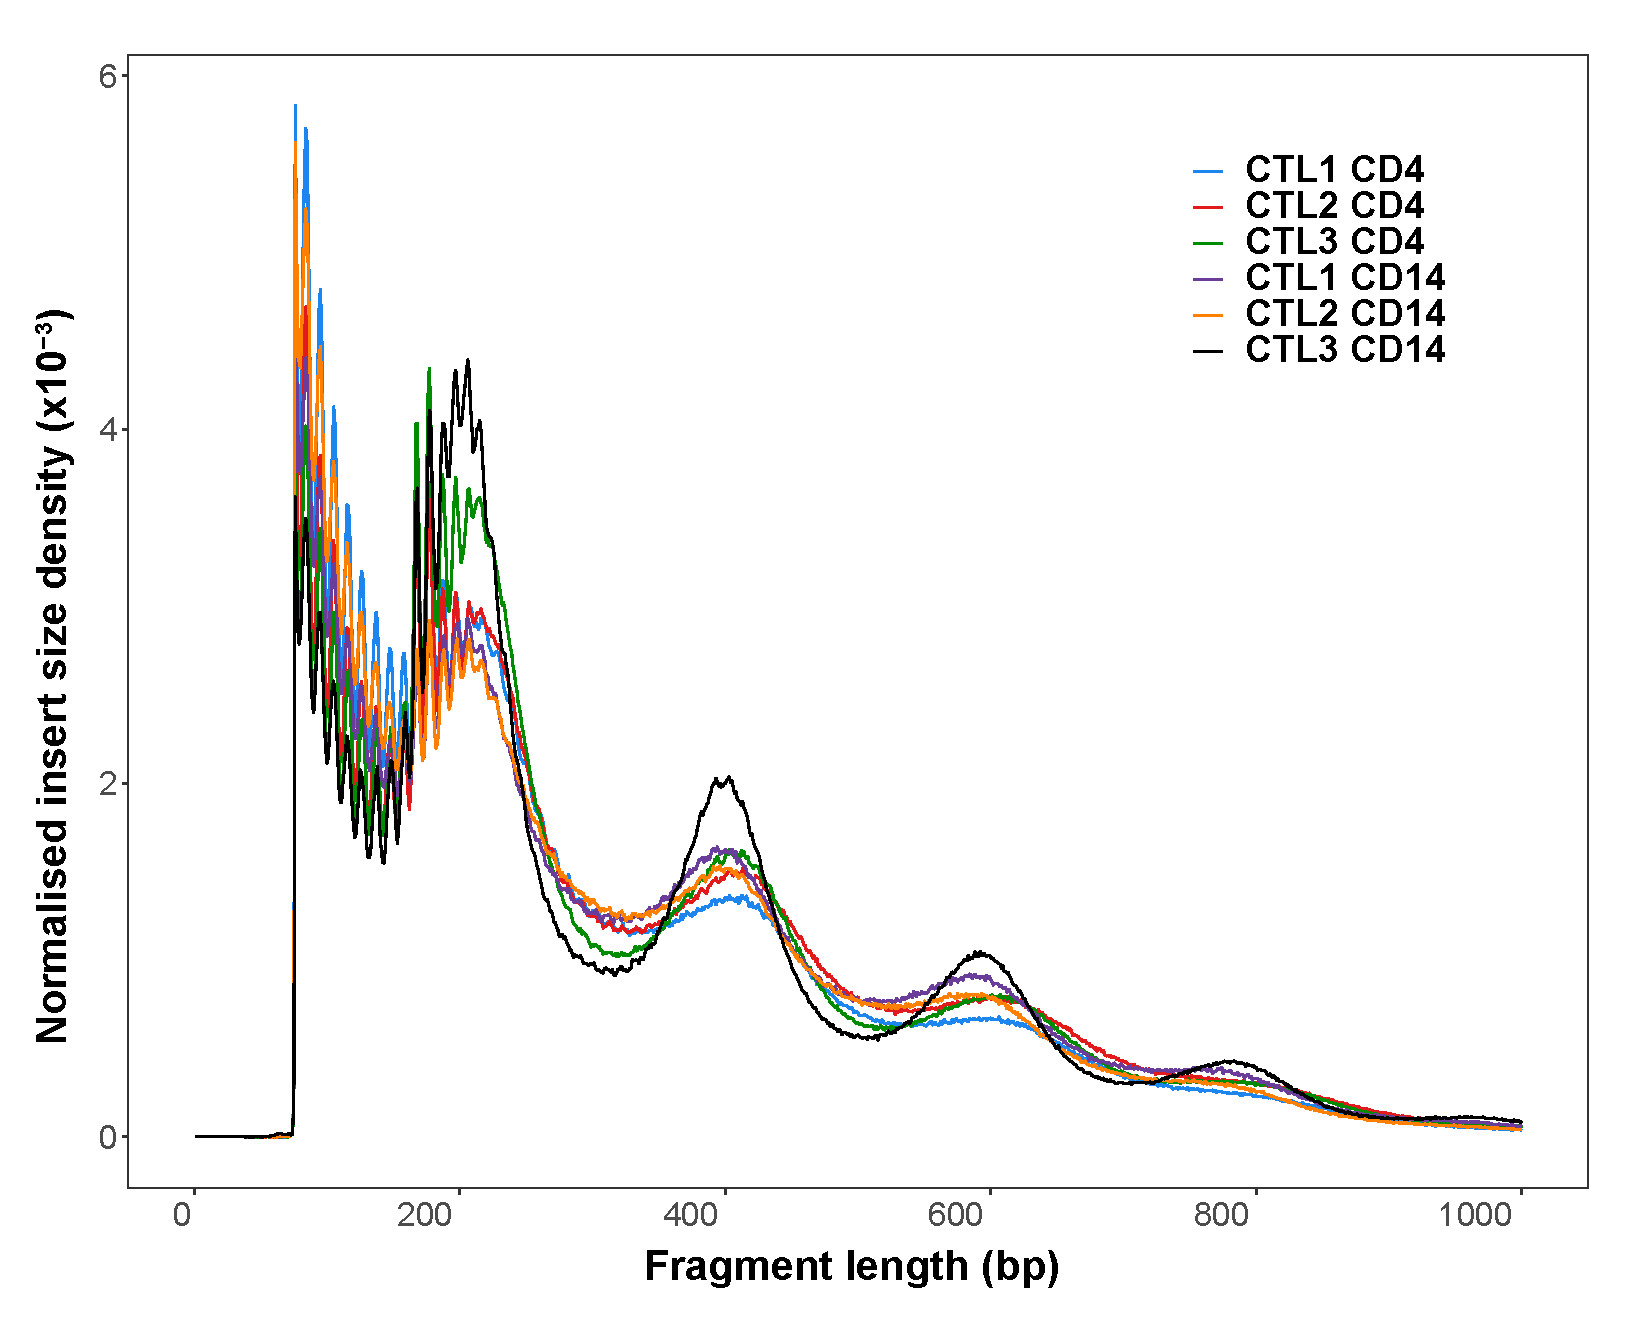
\includegraphics[width=\textwidth]{./Results1/pdfs/ATAC_Core_fresh_CD4_CD14_frag_size_distribution}
\caption{\textbf{}}
\end{subfigure}%
\begin{subfigure}[b]{0.45\textwidth}
\centering
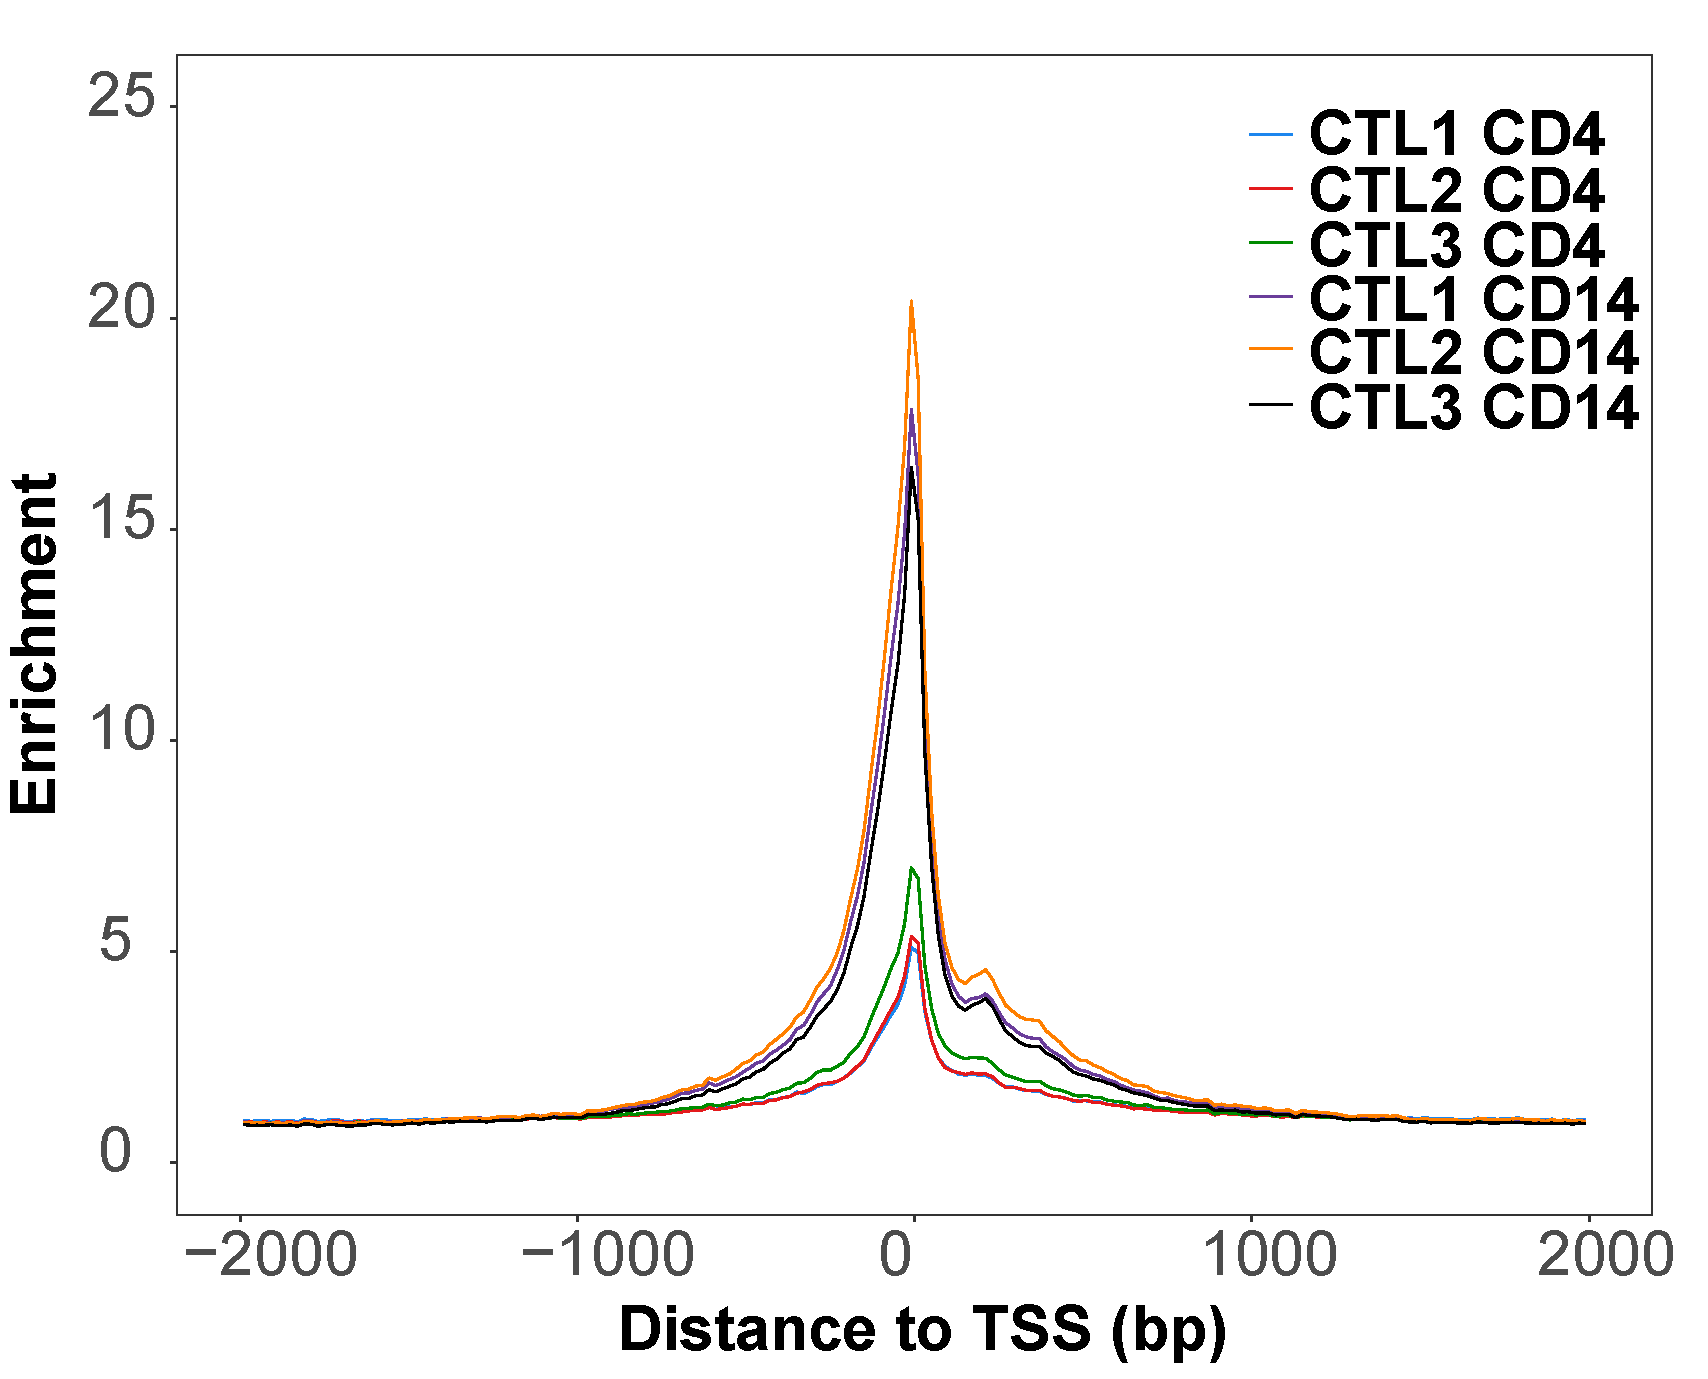
\includegraphics[width=\textwidth]{./Results1/pdfs/TSS_enrichment_Core_fresh_CD4_CD14}
\caption{\textbf{}}
\end{subfigure}
\begin{subfigure}[b]{0.6\textwidth}
\centering
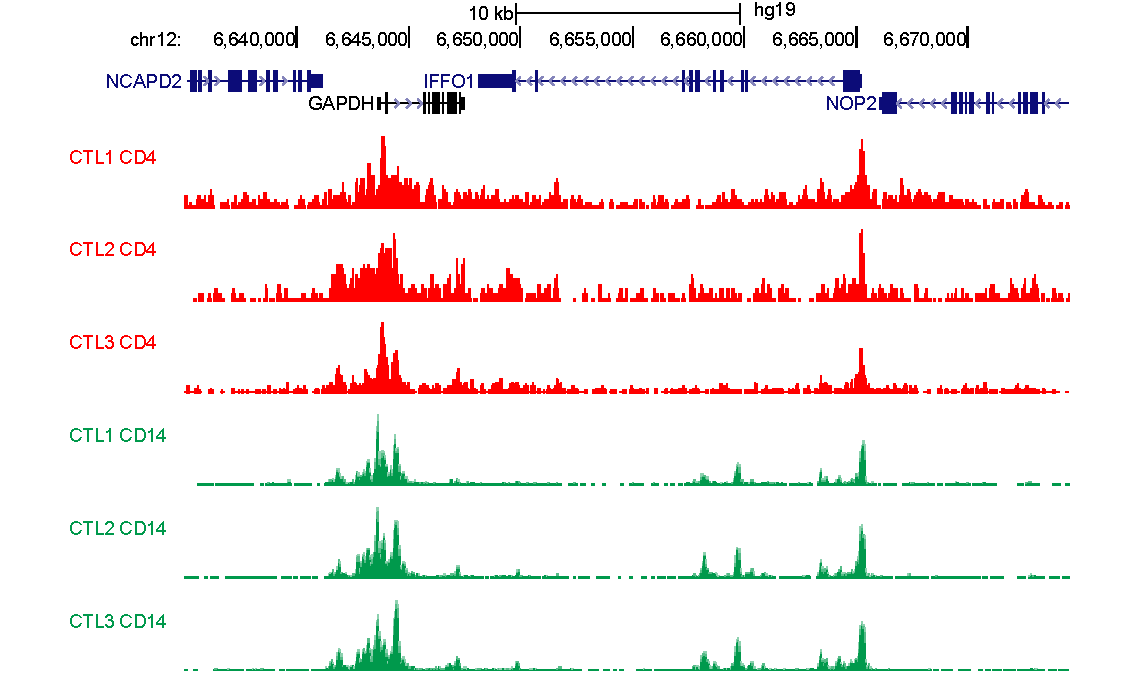
\includegraphics[width=\textwidth]{./Results1/pdfs/ATAC_Core_CD4_CD14_fresh_GAPDH}
\caption{\textbf{}} % to add text to the figure name
\end{subfigure}
\caption[Measurements for quality control assessment in ATAC-seq samples]{\textbf{Measurements for quality control assessment in ATAC-seq samples}}
\label{fig:QC_ATAC}
\end{figure} 



Another QC measurement was the enrichment of ATAC-seq signal over a random background of reads across all the TSS identified for Ensemble genes (Figure \ref{fig:QC_ATAC}b). It is well established that nucleosome repositioning and an increase in chromatin accessibility take place at TSS to allow formation of the transcriptional machinery and initiation of transcription. Fold-enrichment signals ranged between 5-7 for the CD4$^+$ samples and they were much higher(between 17-20) for the CD14$^+$ samples. The lower sample quality of the CD4$^+$compared to CD14$^+$ shown by the TSS signal were recapitulated by the ATAC-seq signal at the promoter of the constitutively expressed gene glyceraldehyde-3-phosphate dehydrogenase (\textit{GAPDH}) (Figure \ref{fig:QC_ATAC}c). 
	
As part of the QC assessment I looked at the percentage of mitochondrial reads and the fraction of reads in peaks (FRiP)(Table \ref{tab:ATAC_MT_fraction_reads_in_peaks}). 

\begin{table}[htbp]
%\setlength{\tabcolsep}{20pt} only to stretch the columns if you want
%\renewcommand{\arraystretch}{1.5}
\centering
\begin{tabular}{@{} c c c}
\toprule
\textbf{Sample} & \textbf{\% MT reads} & \textbf{Fraction of reads in peaks} \\
\midrule
\midrule
CTL1 CD4 & 14.9 & 9.8 \\
CTL2 CD4 & 30.5 & 11.2 \\
CTL3 CD4 & 28.8 & 11.6 \\
CTL1 CD14 & 43.3 & 32.2 \\
CTL2 CD14 & 36.8 & 57.0 \\
CTL3 CD14 & 37.6 & 49.9 \\
\bottomrule
\end{tabular}
\medskip %gap
\caption[ATAC-seq percentage of MT reads and fraction of reads in called peaks]{\textbf{}}
\label{tab:ATAC_MT_fraction_reads_in_peaks}
\end{table}
\bigskip %bigger space


FRiP score is a way of assessing the background signal in different types of assays that are based on peak calling, including ChIP-seq. Positive correlation between the TSS fold-change enrichment and FRiP was observed (data not shown), being both appropriate inter-dependent QC measures to evaluate sample noise. Regarding TSS and FRiP cut-off values, Alsoo \textit{et al.}, 2018 and, recently, ENCODE have recommended minimum FRiP between 10-20\% and TSS between 6-10. ENCODE has prioritised the use of TSS over FRiP as the measurement to determine the noise in the sample \parencite{ENCODE}. According to this recommendations all these samples passed QC; however clear differences were seen between CD4$^+$ and CD14$^+$ samples. The mitochondrial content ranged between 14.9-43.3\% and, alike FRiP and TSS, it was higher in CD14$^+$ than in CD4$^+$ and not directly related with any of the other QC measurements.


	

\subsubsection{Peak calling and filtering}
As part of the ATAC-seq pipeline implementation, peak calling and the criteria for filtering where another two aspects to determine.
Although different peak callers have been used, most of the publications as well as ENCODE has been using MACS2 as the preferred methodology (Table \ref{tab:ATAC_comparative_methods}). MACS2 has been initially developed for ChIP but it has also been used for DHS and ATAC-seq with disabling the model and agreeing in an extension size (--extsize) and a shift (--shift), which indicate the direction and number of bp for reads to be shifted and the number of bp for them to be extended, respectively. The --extsize should correspond to the average fragment size, which in my libraries is $\sim$200bp and the --shift is set to -100, as it is recommended to be set to -1/2 of the fragment size for chromatin accessibility assays. This parameter could be further optimised but it escapes from the aim of this thesis.

I was interested in understanding the effect of sequencing depth and the sample quality on the peak calling to have a better control of both variables in the downstream analysis. I performed random read sub-sampling every 5M total reads (from 5M to 30M) followed by peak calling with arbitrary filtering for FDR$<$0.01 in each of the six aforementioned samples. 

The number of called peaks passing filtering showed an steady increased over the read depth which seemed to reach a \textit{plateau} around 25M reads (Figure \ref{fig:Peak_calling_versus_depth_ATAC}a). This was consistent with the decay in the increments of called peaks over read depth, almost invariable, from 20M reads onwards (Figure \ref{fig:Peak_calling_versus_depth_ATAC}b). Moreover, lower number of peaks were detected in CD4$^+$ samples compared to CD14$^+$ highlighting the influence of sample quality on the total number of called peaks. Interestingly, sample quality measured by FRiP reflected very low changes over read depth and was stable from 15M reads for all six samples (Figure \ref{fig:Peak_calling_versus_depth_ATAC}c). Overall, this confirmed that measurement of sample quality by FRiP or TSS is not biased by sequencing depth.


\begin{figure}[htbp]
\centering
\begin{subfigure}{0.50\textwidth}
\centering
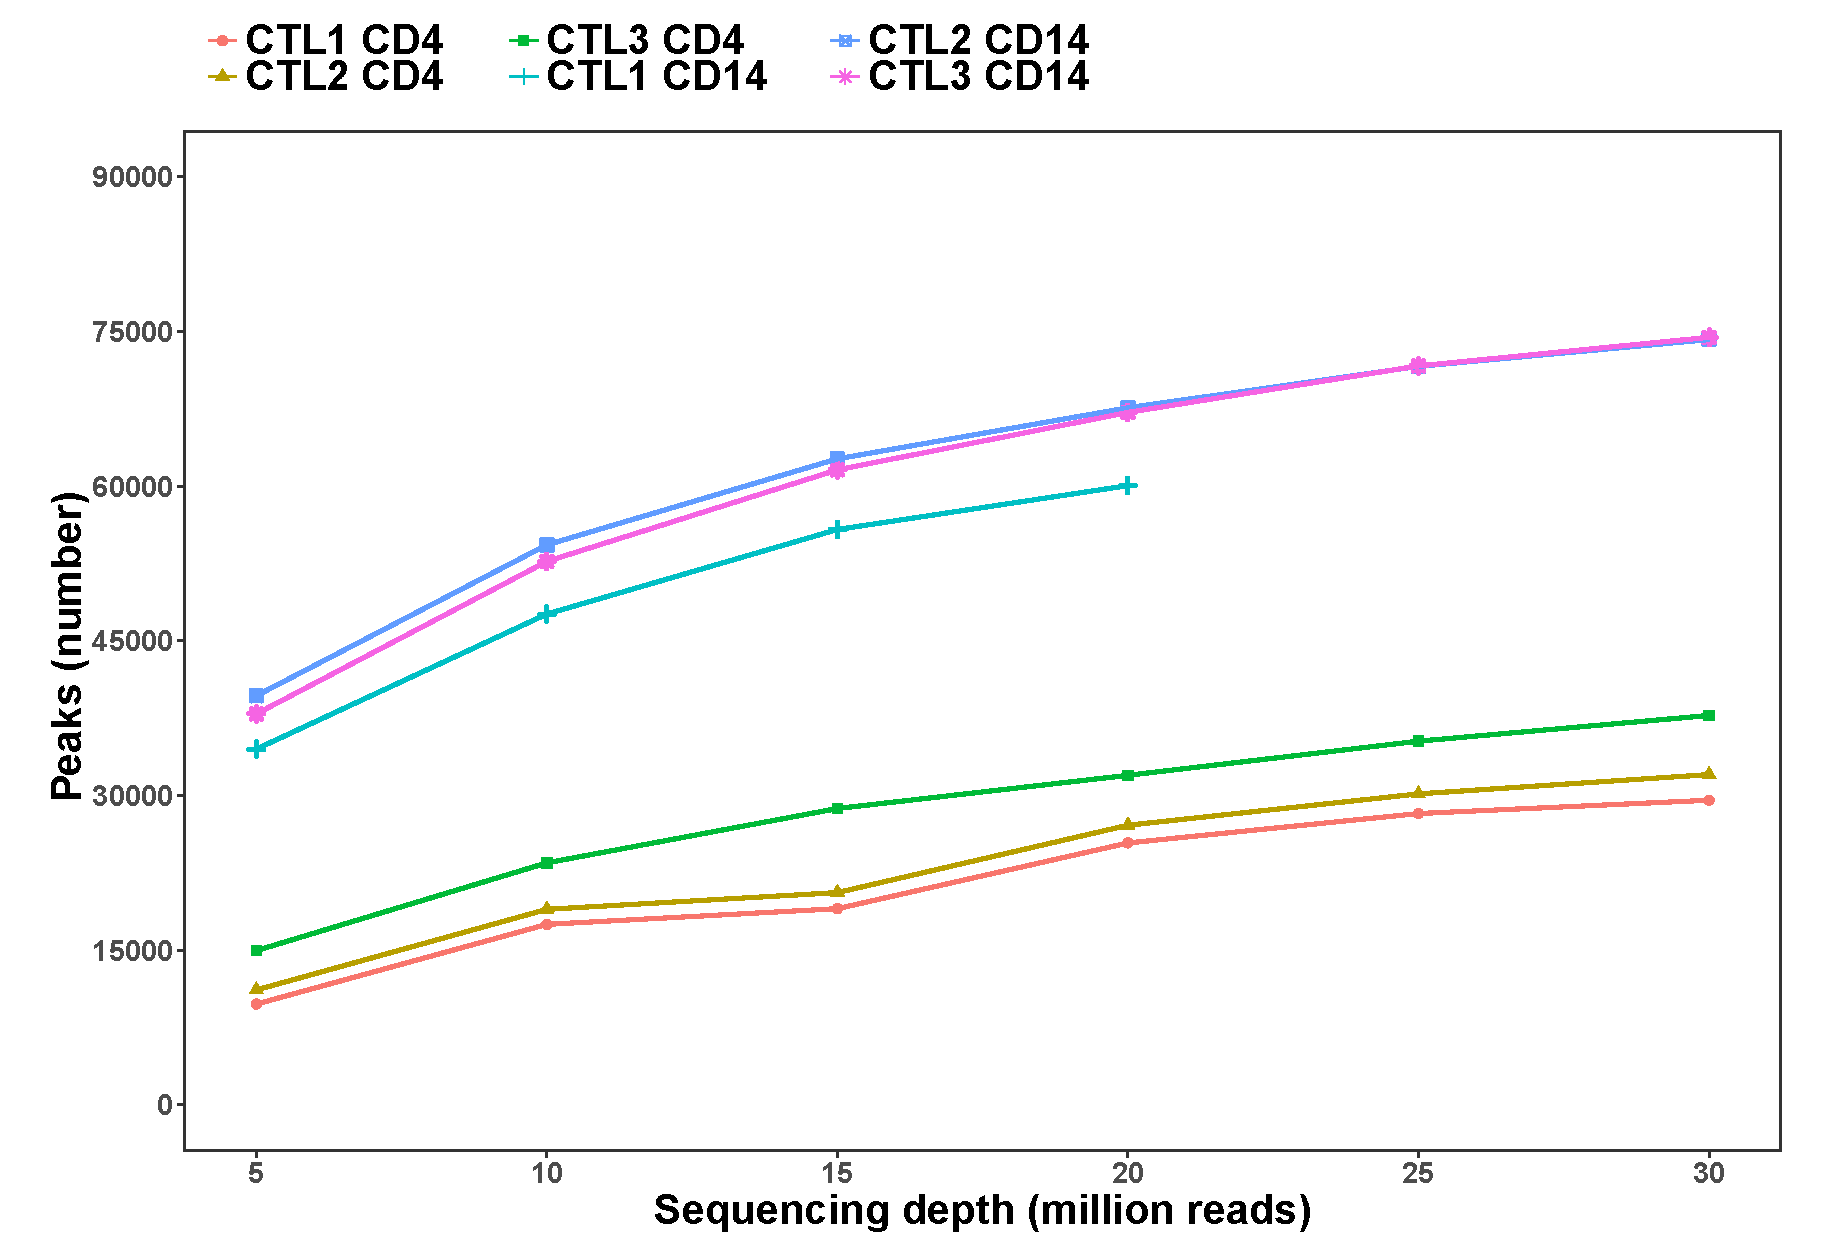
\includegraphics[width=\textwidth]{./Results1/pdfs/ATAC_Core_fresh_CD4_CD14_num_peaks_vs_depth}
\caption{\textbf{}}
% The percentage sign indicated that the other subfig goes side by side
\end{subfigure} \\
\begin{subfigure}{0.45\textwidth}
\centering
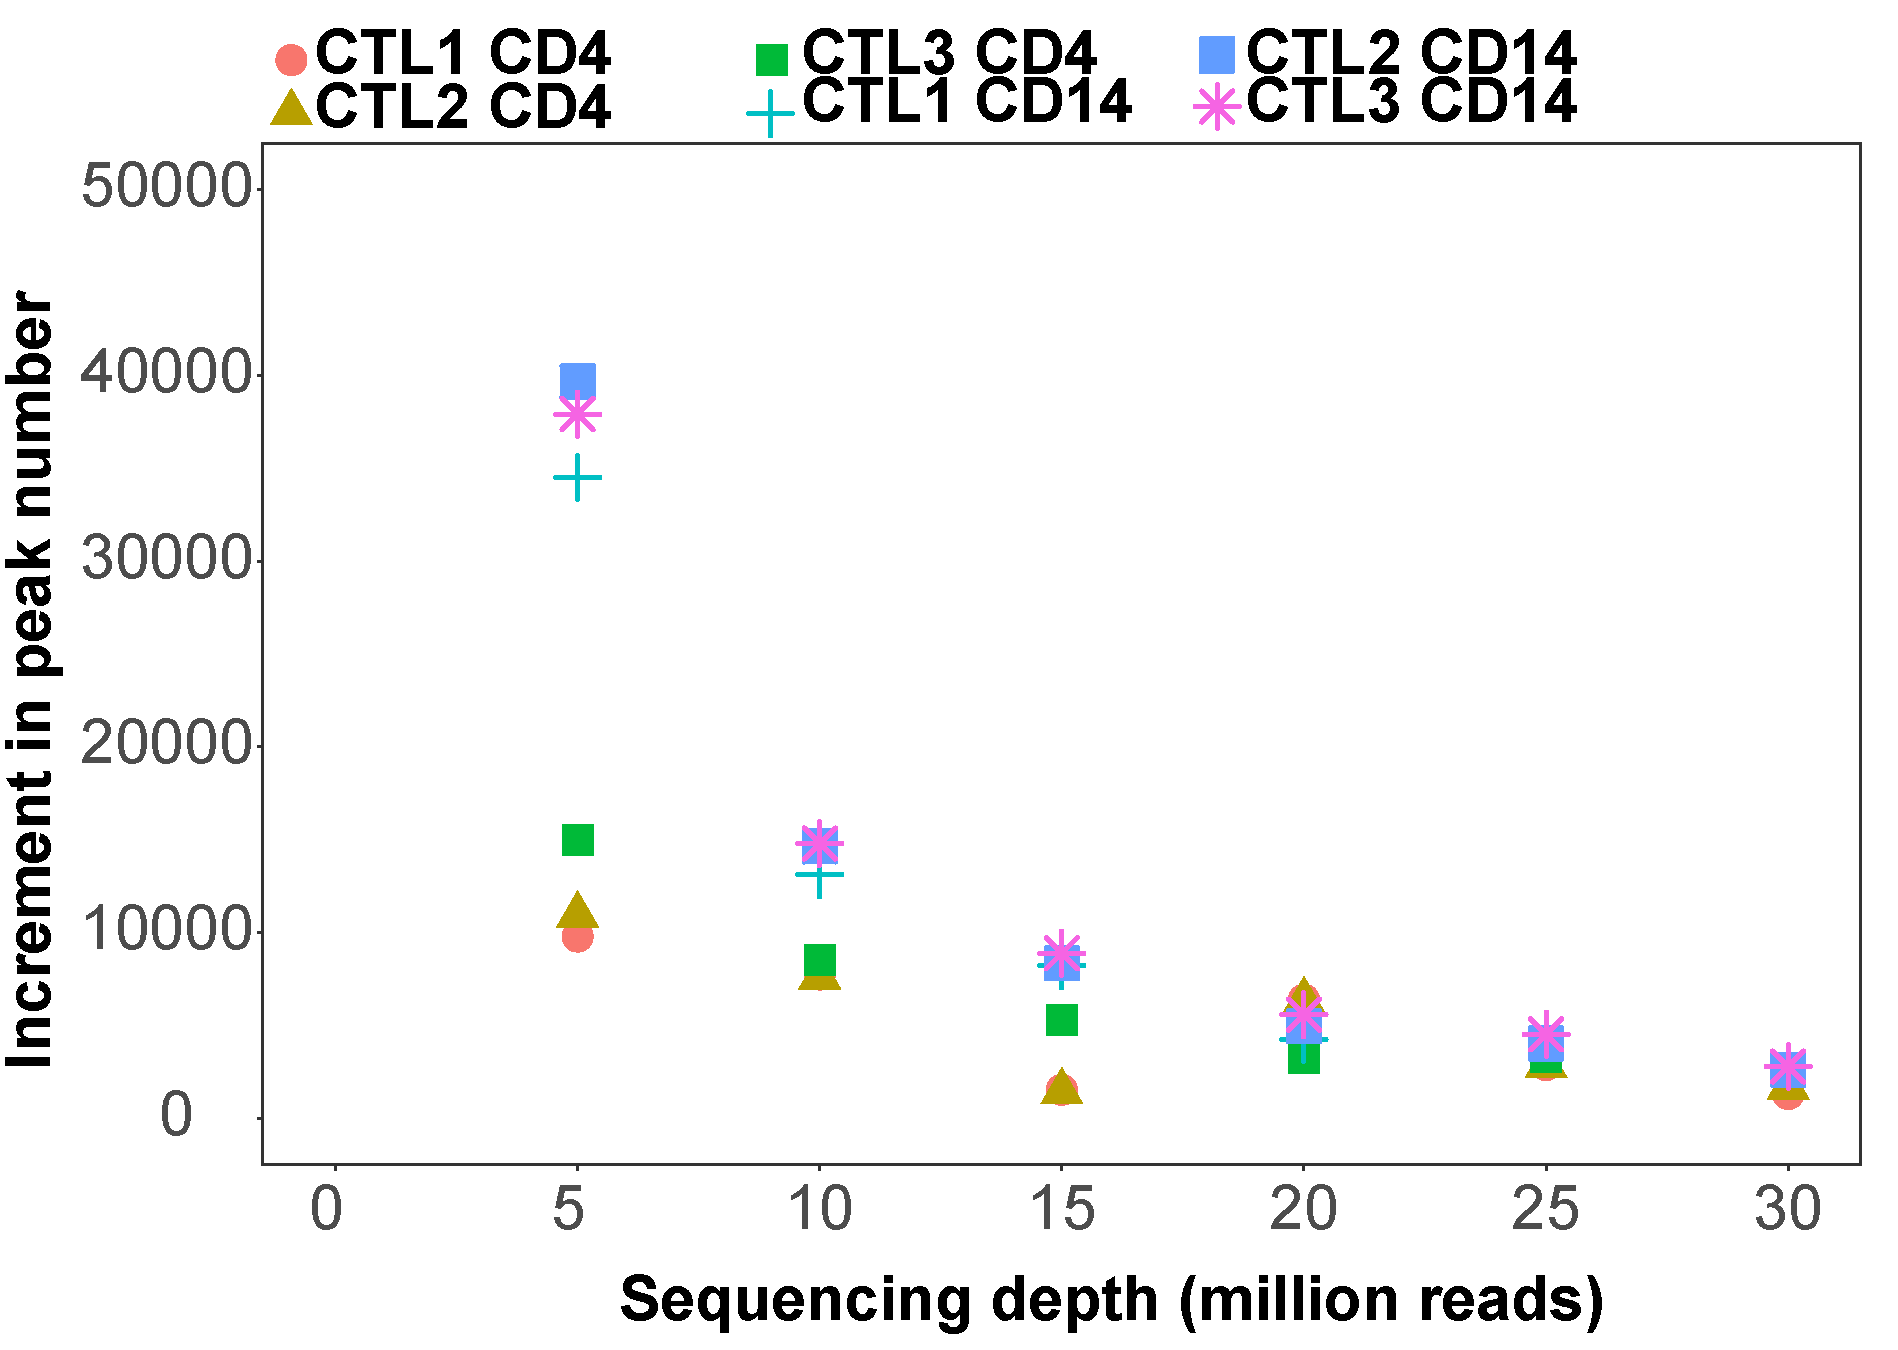
\includegraphics[width=\textwidth]{./Results1/pdfs/ATAC_Core_fresh_CD4_CD14_increment_num_peaks_vs_depth}
\caption{\textbf{}}
\end{subfigure} %
\begin{subfigure}{0.45\textwidth}
\centering
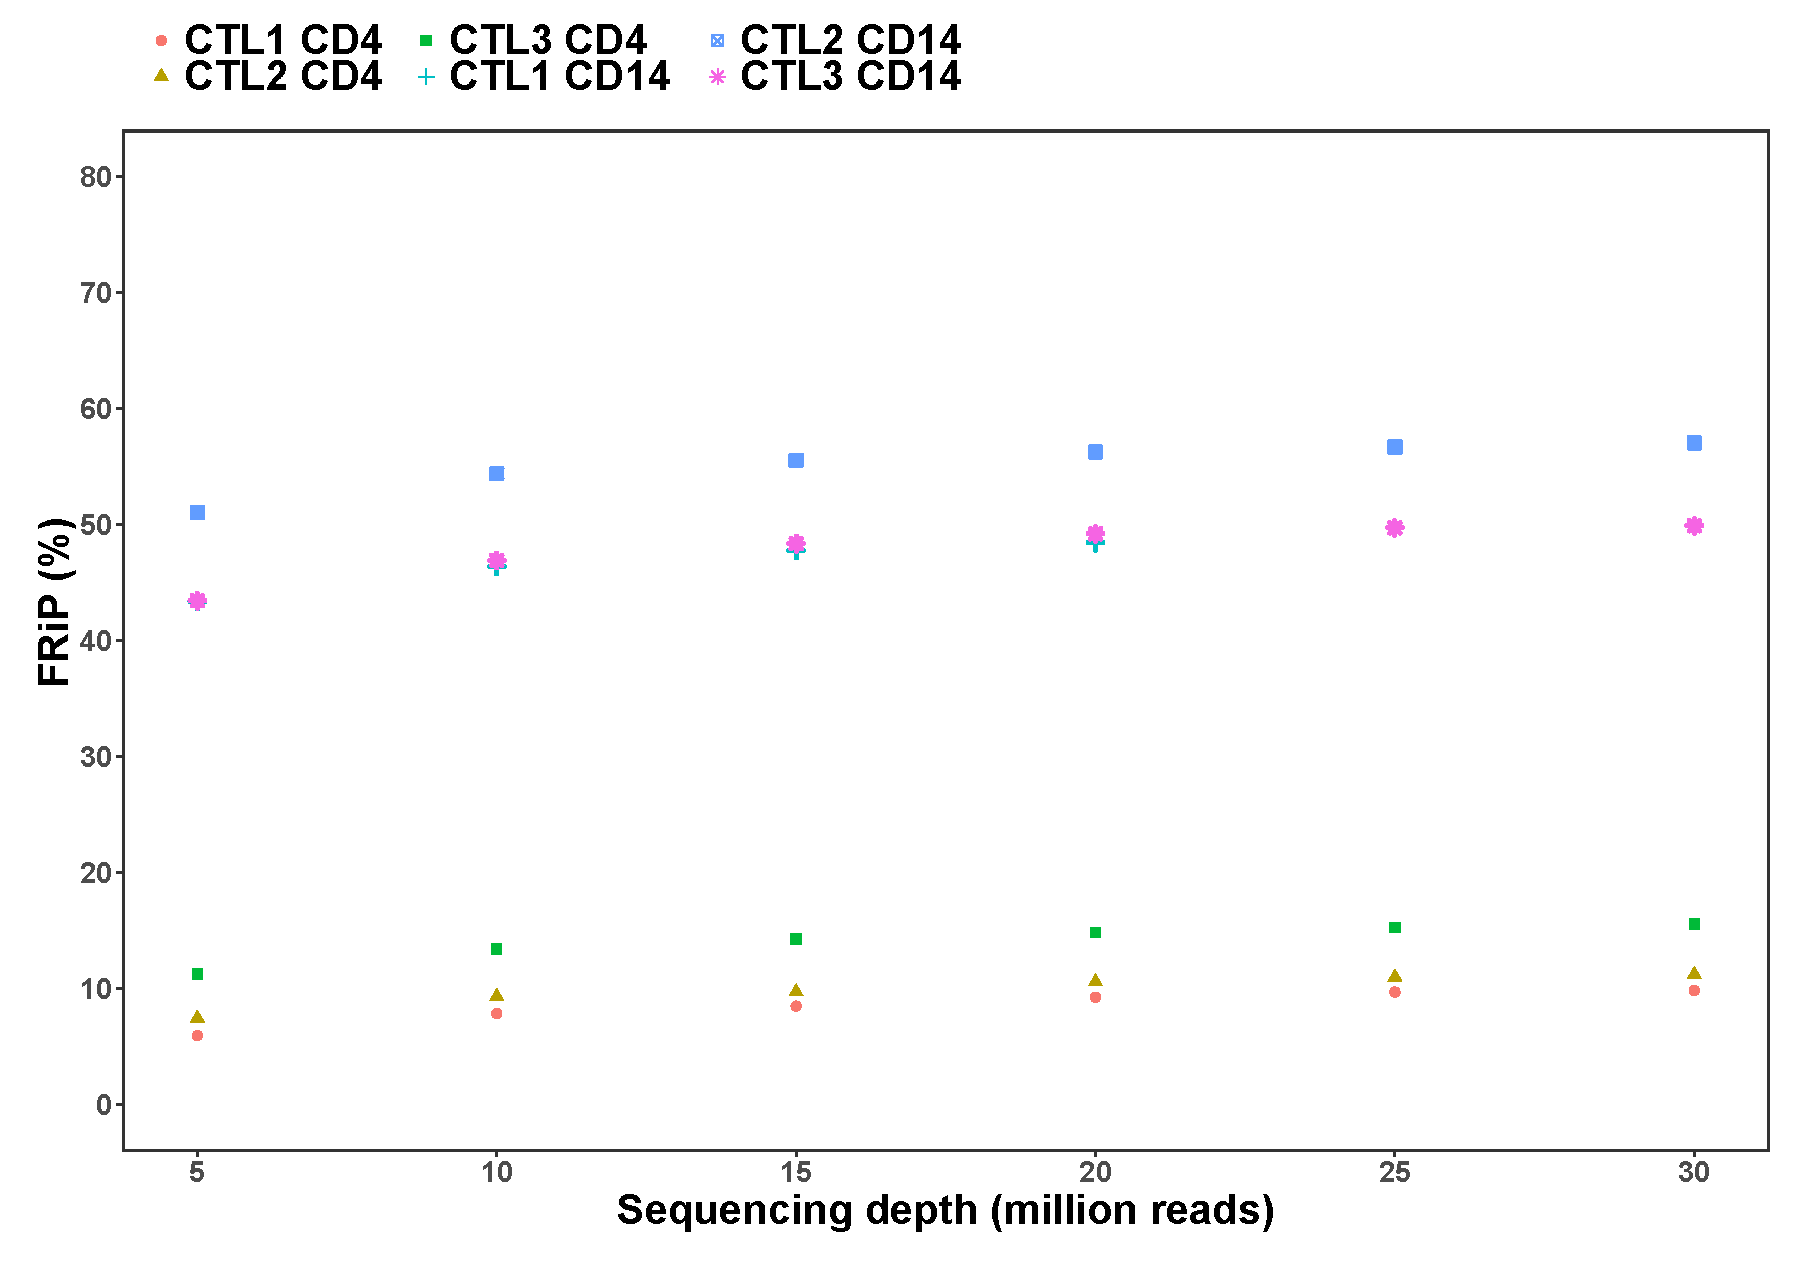
\includegraphics[width=\textwidth]{./Results1/pdfs/ATAC_Core_fresh_CD4_CD14_frac_reads_in_peaks_vs_depth}
\caption{\textbf{}}
\end{subfigure}
\caption[Peak calling and sequencing depth in ATAC-seq samples]{\textbf{Peak calling at different sequencing depth in ATAC-seq samples} \\
}
\label{fig:Peak_calling_versus_depth_ATAC}
\end{figure} 



Regarding peak calling filtering, most of the ATAC-seq publications using MACS2 have arbitrarily used an FDR$<$0.01 (Table \ref{tab:ATAC_comparative_methods}). In collaboration with Dr. Gabriele Migliorini and following ENCODE pipeline, we explored the use of IDR to experimentally identify the most appropriate p-val for filtering each individual sample. Each sample was partitioned in two, peaks were called in each half and the percentage of peaks (over the total number shared peaks) sharing IDR at a particular p-val was calculated (Figure \ref{fig:Peak_calling_IDR_filtering_and_chrom_stated_ATAC} a and b). Both of the representative samples showed variation in the percentage of shared peaks upon sequencing depth under 10M reads, being the effect more pronounced and extended in the lower quality (CTL2 CD4$^+$ Figure \ref{fig:Peak_calling_IDR_filtering_and_chrom_stated_ATAC} a) compared to the counterpart CD14$^+$ (Figure \ref{fig:Peak_calling_IDR_filtering_and_chrom_stated_ATAC} b). The shape of the curves was also influenced by the sample quality, presenting a smoother profile reaching a single maximum percentage of shared IDR peaks for samples with TSS enrichment $>\sim$10 compared to samples with lower quality. All the CD14$^+$ samples reached the maximum percentage of IDR shared peaks at approximately -log10 pval 8 (data not shown). 
Filtering the CD4$^+$ peaks at the -log10 pval of the first maximum of IDR shared peaks reduced the percentage of peaks overlapping noise ( e.g heterochromatin, repetitive sequences and repressed regions) when compared to peaks filtered based on FDR$<$0.01 (Figure \ref{fig:Peak_calling_IDR_filtering_and_chrom_stated_ATAC} b). In summary, this IDR analysis appeared as systematic method to identify an optimum p-val to perform individual filtering in a sample-specific manner and in a less arbitrary way than the extended 1\% FDR. 

%Should mention that the median of all this first max are used to perform filtering for all the samples because following other pipelines they always use same filtering value for all samples so we need to be consistent across samples



\begin{figure}[htbp]
\centering
\begin{subfigure}{0.5\textwidth}
\centering
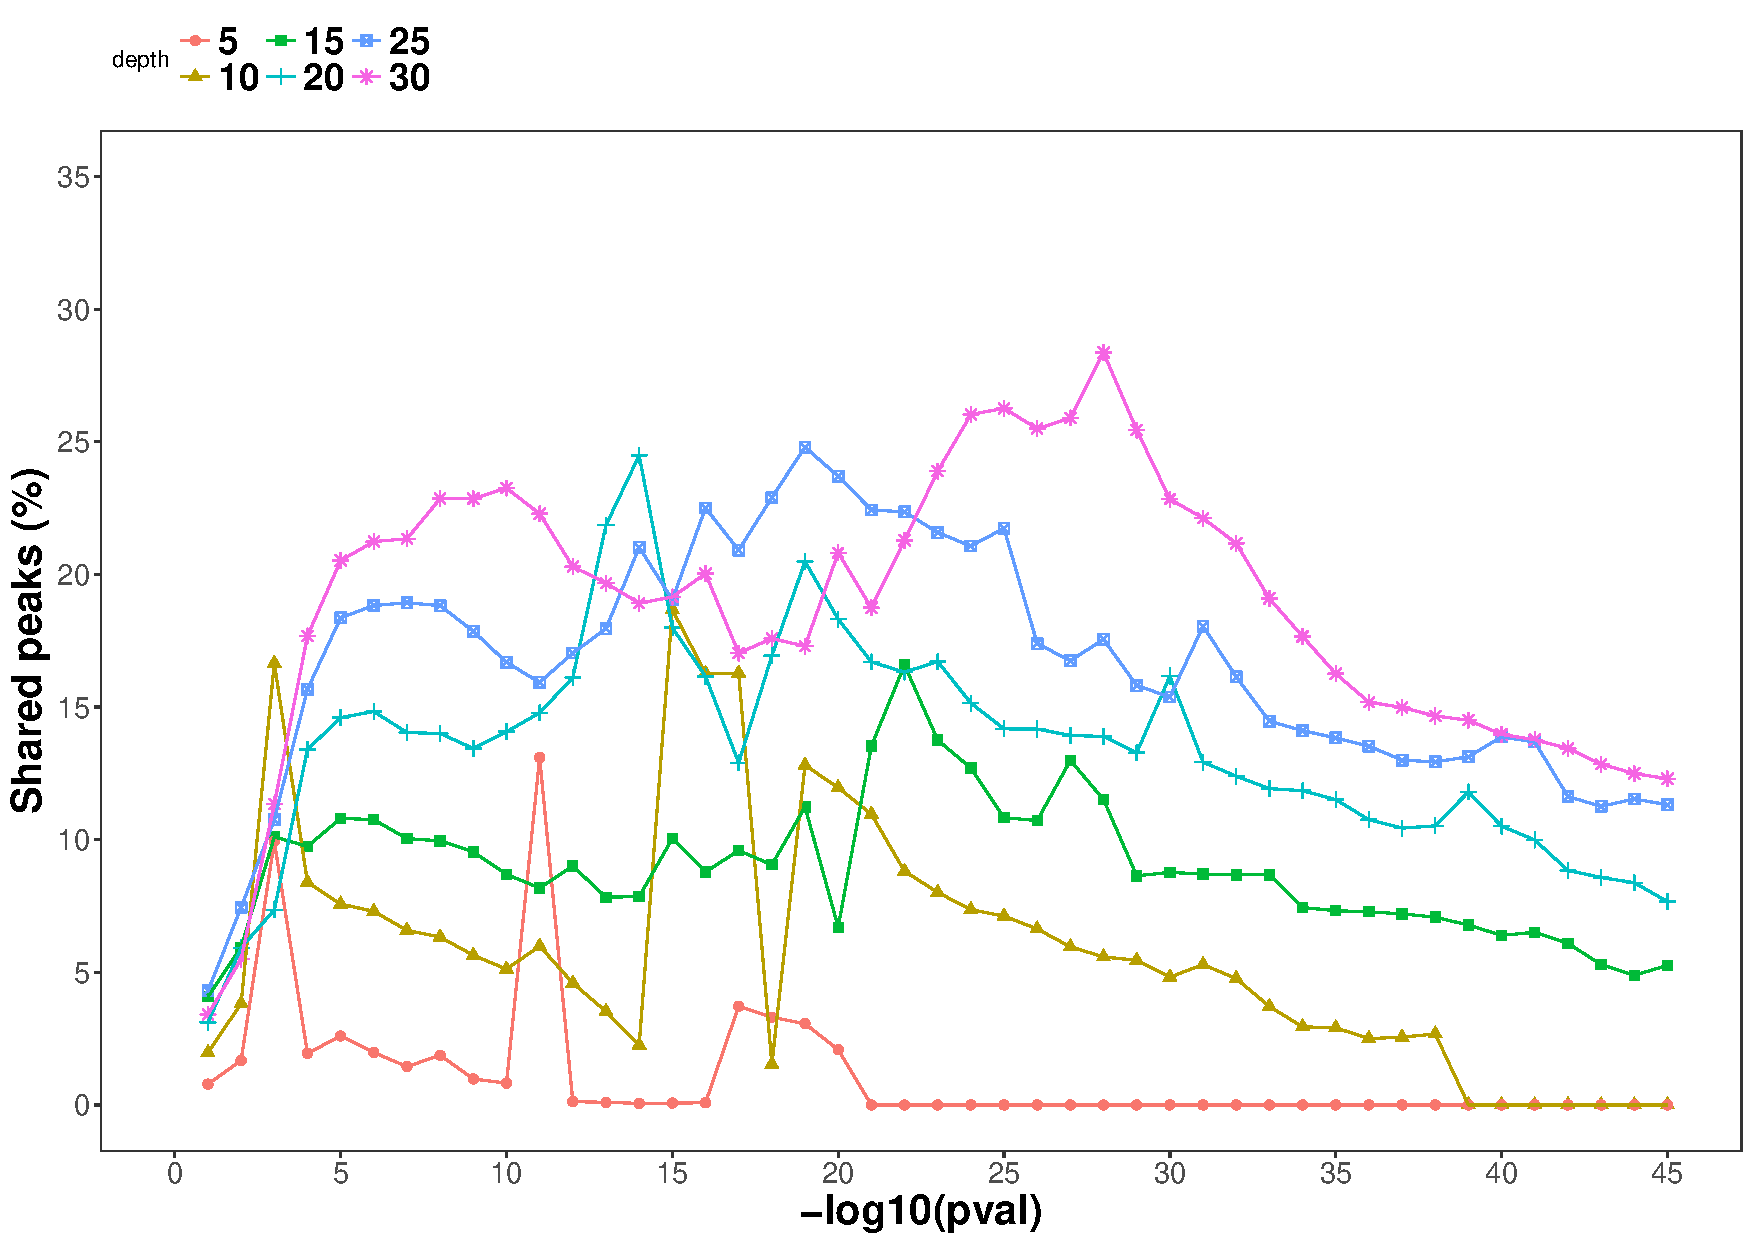
\includegraphics[width=\textwidth]{./Results1/pdfs/ATAC_Core_fresh_CTL2_CD4_shared_peaks_IDR_vs_pval}
\caption{\textbf{}}
% The percentage sign indicated that the other subfig goes side by side
\end{subfigure}%
\begin{subfigure}{0.5\textwidth}
\centering
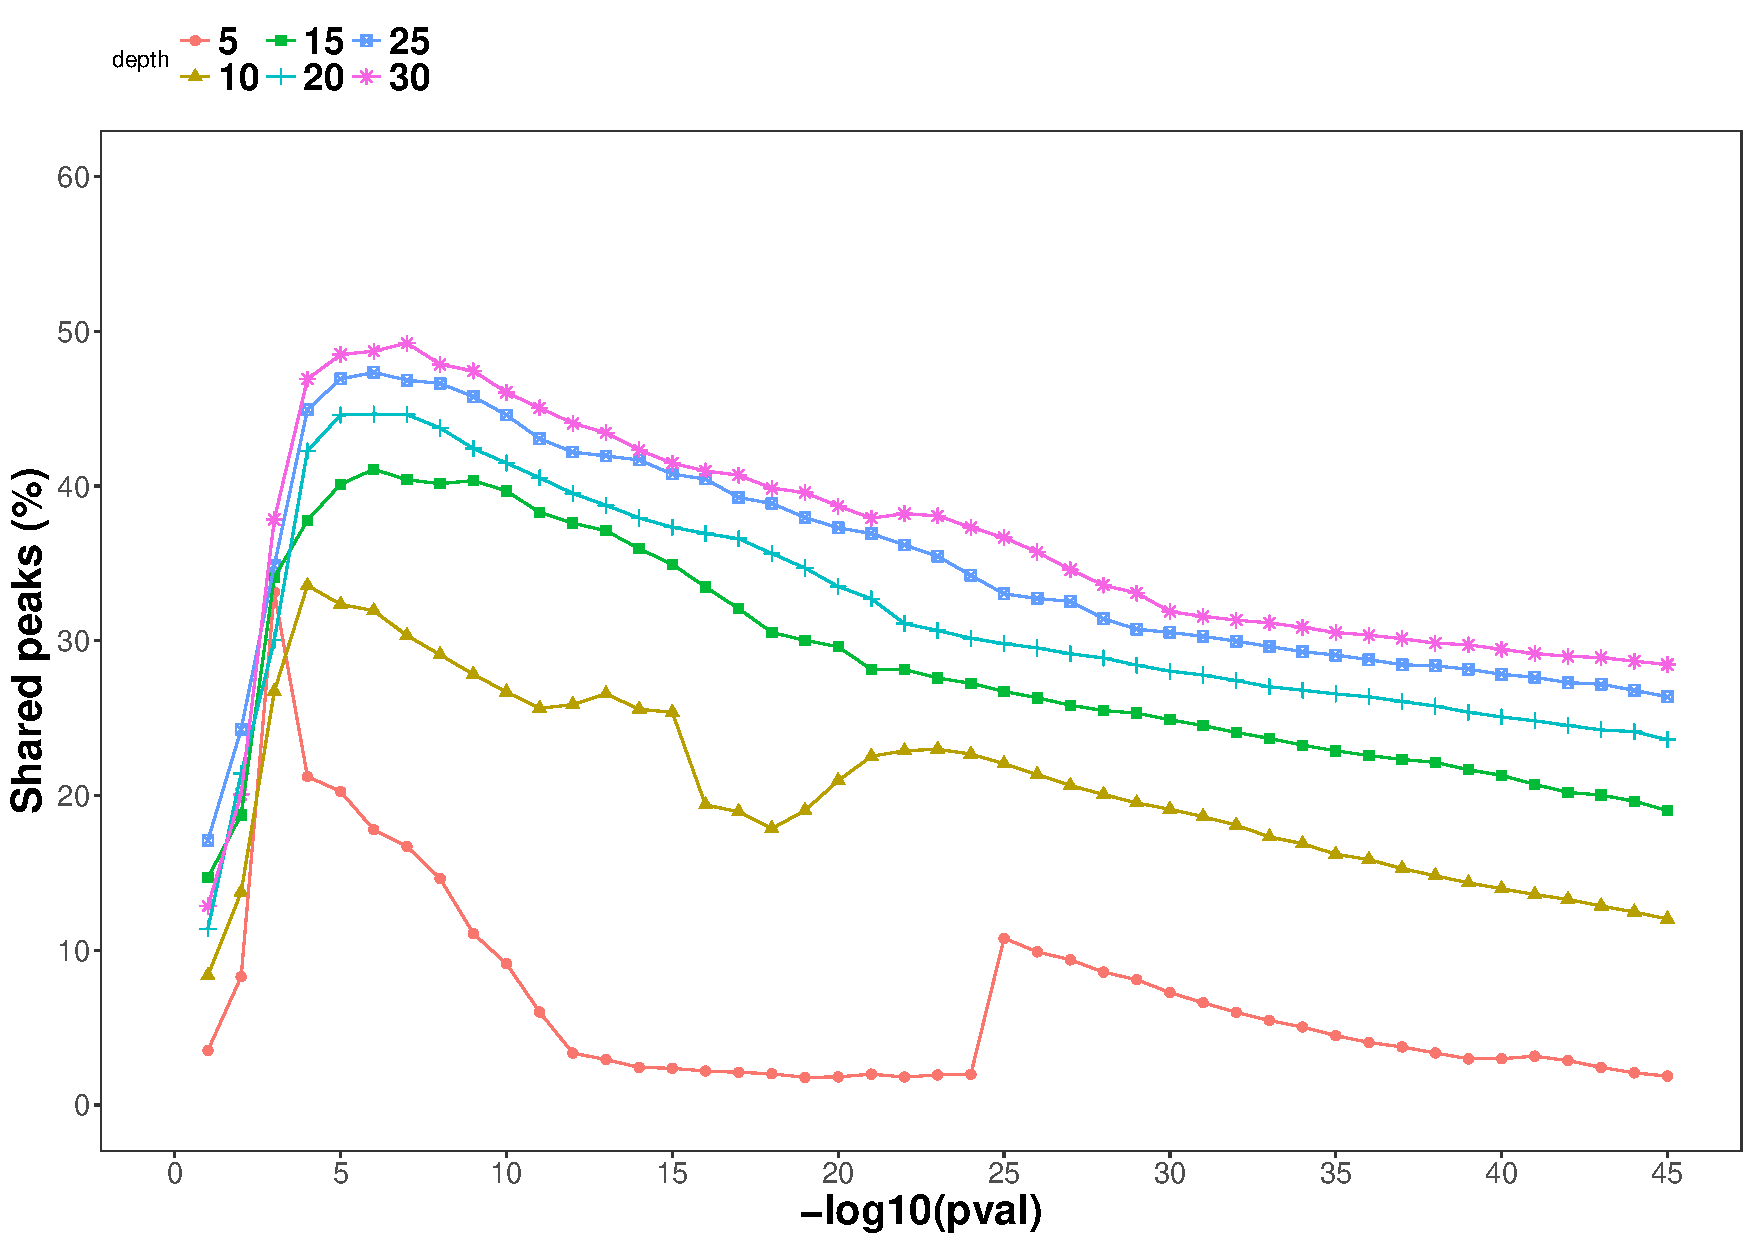
\includegraphics[width=\textwidth]{./Results1/pdfs/ATAC_Core_fresh_CTL2_CD14_shared_peaks_IDR_vs_pval}
\caption{\textbf{}}
\end{subfigure} \\
\begin{subfigure}{0.65\textwidth}
\centering
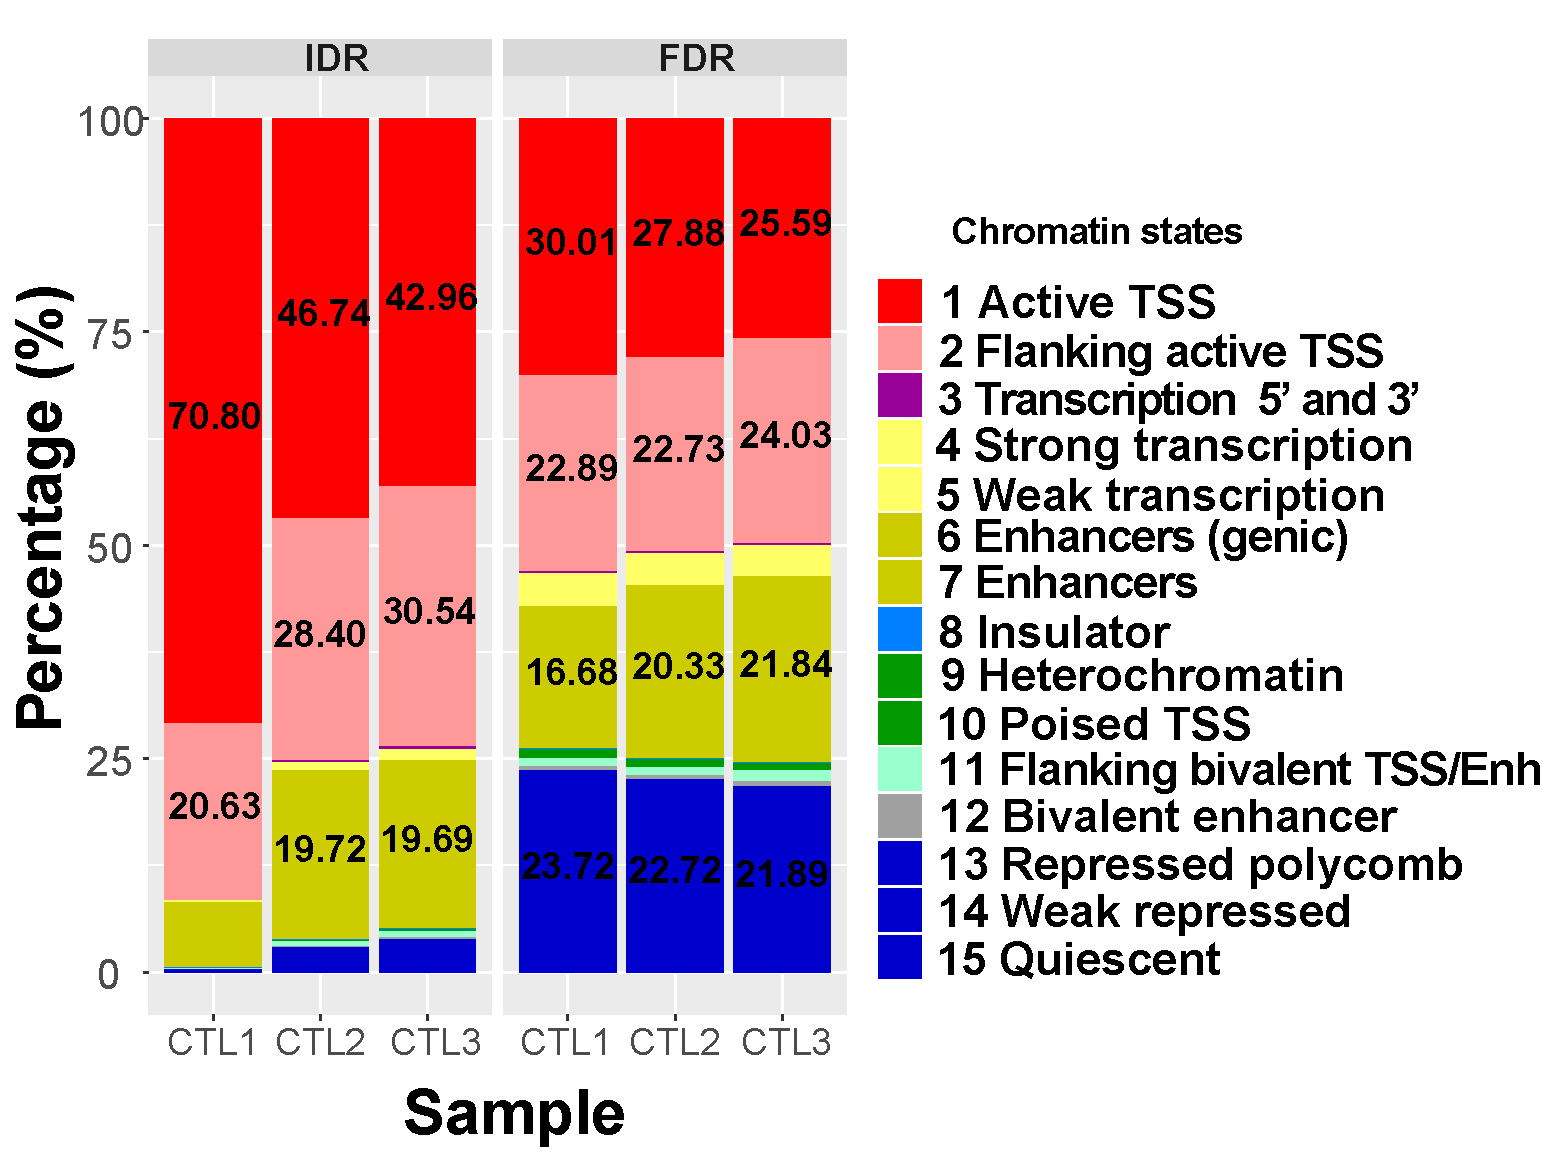
\includegraphics[width=\textwidth]{./Results1/pdfs/stacked_barplot_chromatin_states_percent_CD4_qval_vs_PVAL_IDR_filtered}
\caption{\textbf{}} % to add text to the figure name
\end{subfigure}%
\caption[Peak calling filtering using IDR analysis in ATAC-seq samples]{\textbf{Peak calling filtering using IDR analysis in ATAC-seq samples}}
\label{fig:Peak_calling_IDR_filtering_and_chrom_stated_ATAC}
\end{figure} 




\subsubsection{Differential chromatin accessibility analysis}

From the methods that can be used to perform differential chromatin accessibility analysis (Table \ref{tab:ATAC_comparative_methods}), I chose a peak-based approach where a consensus master list between all samples was built and the number of reads overlapping the master list peaks were retrieved for each sample. As previously mentioned in the Chapter \label{ch:Mat} the master list was composed of non-overlapping 500bp with peaks present in at least 30\% of the samples, regardless the group they belonged to (e.g patients or controls). One of the main limitations of the ATAC-seq and FAST-ATAC protocols (discussed in the next section) is the background signal. Therefore, it was calculation of an empirical cut-off, similarly to the strategy use in micro-array technology, was performed to minimise the impact of background read counts on the differential analysis \parencite{Xinmin2005,Jonker2014}. Moreover, due to the lack of consistency found across the ATAC-seq publications, two methods for normalisation/differential analysis were assayed.

From the count matrix of the same six samples as before, the combined distribution of read density from all the absent peaks in each sample was used to define a sequence of twenty cut-offs. These cut-offs corresponded to the number of counts showed by a particular percentage of absent peaks (supplementary info). Each cut-off was used to filter out from the raw count matrix those peaks from the master list for which the number of counts was $<=$ than that particular cut-off in more than three samples  (being three the number of the smallest group of replicates in this particular experimental design). Quantile normalisation followed by differential analysis with limma voom showed greater number of differential open chromatin regions (DOCs) at an FDR$<$0.01 compared to DESeq2 across all the cut-offs (Figure \ref{fig:DOC_quantile_DESeq2} a). The two approaches presented progressive decrease in the number of DOC sites from the 75\% cut-off. Conversely, the proportion of DOC calculated over the total number of regions considered in the differential analysis for each cut off significantly increased from the 50\% cut-off onwards, indicating a progressive reduction in the false positive hits reported \ref{fig:DOC_quantile_DESeq2} b). 
From this analysis, 80\% was chosen as a conservative filtering cut-off for which almost all the 19,855 DOCs identified by the most conservative method (DESeq2) at an FDR$<$0.01 were recapitulated by limma voom at the same FDR (Figure \ref{fig:DOC_quantile_DESeq2} c). 

\begin{figure}[htbp]
\centering
\begin{subfigure}{0.45\textwidth}
\centering
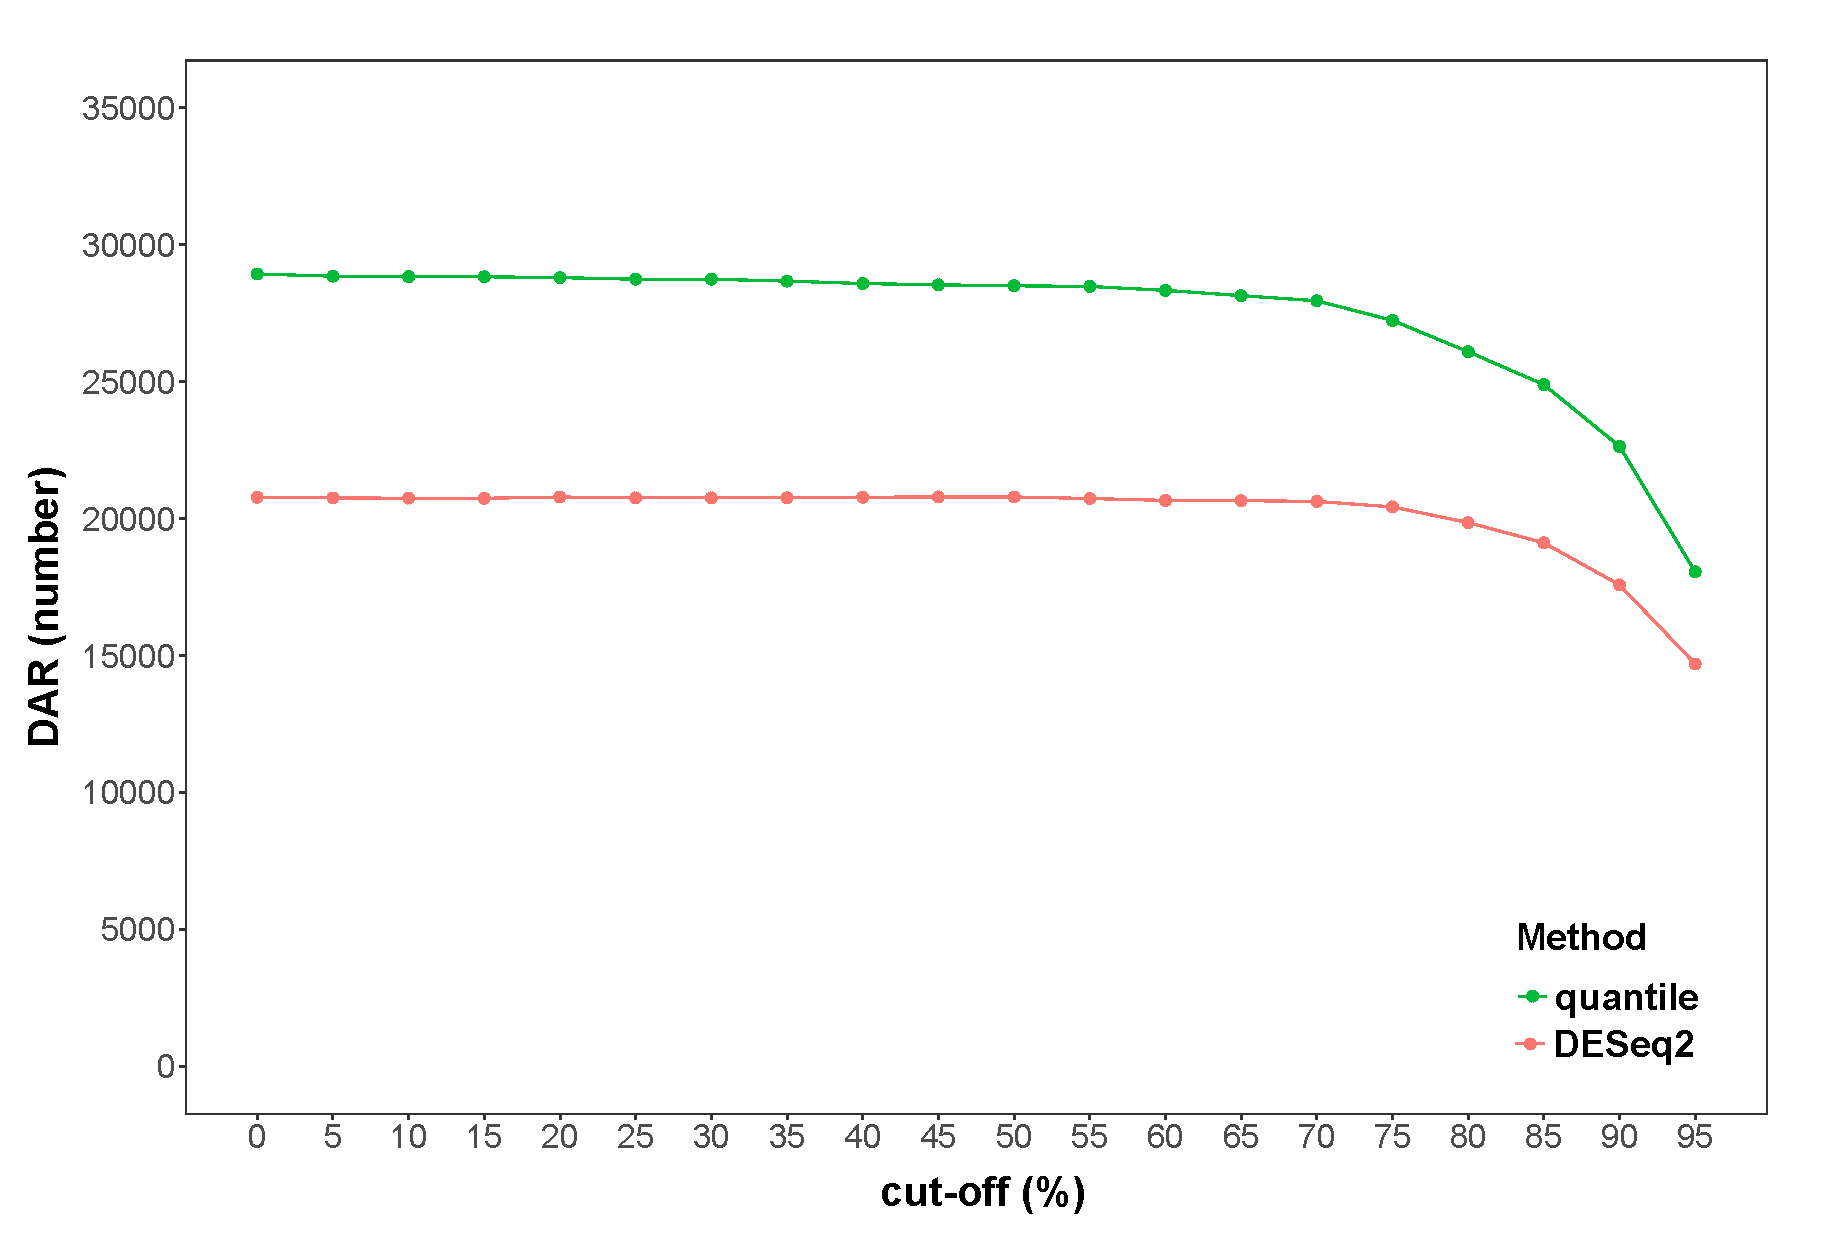
\includegraphics[width=\textwidth]{./Results1/pdfs/ATAC_Core_CD4vsCD14_DOC_FDR_01_vs_cutoffs_quantile_DESeq2_only}
\caption{\textbf{}}
\end{subfigure}%
\begin{subfigure}{0.45\textwidth}
\centering
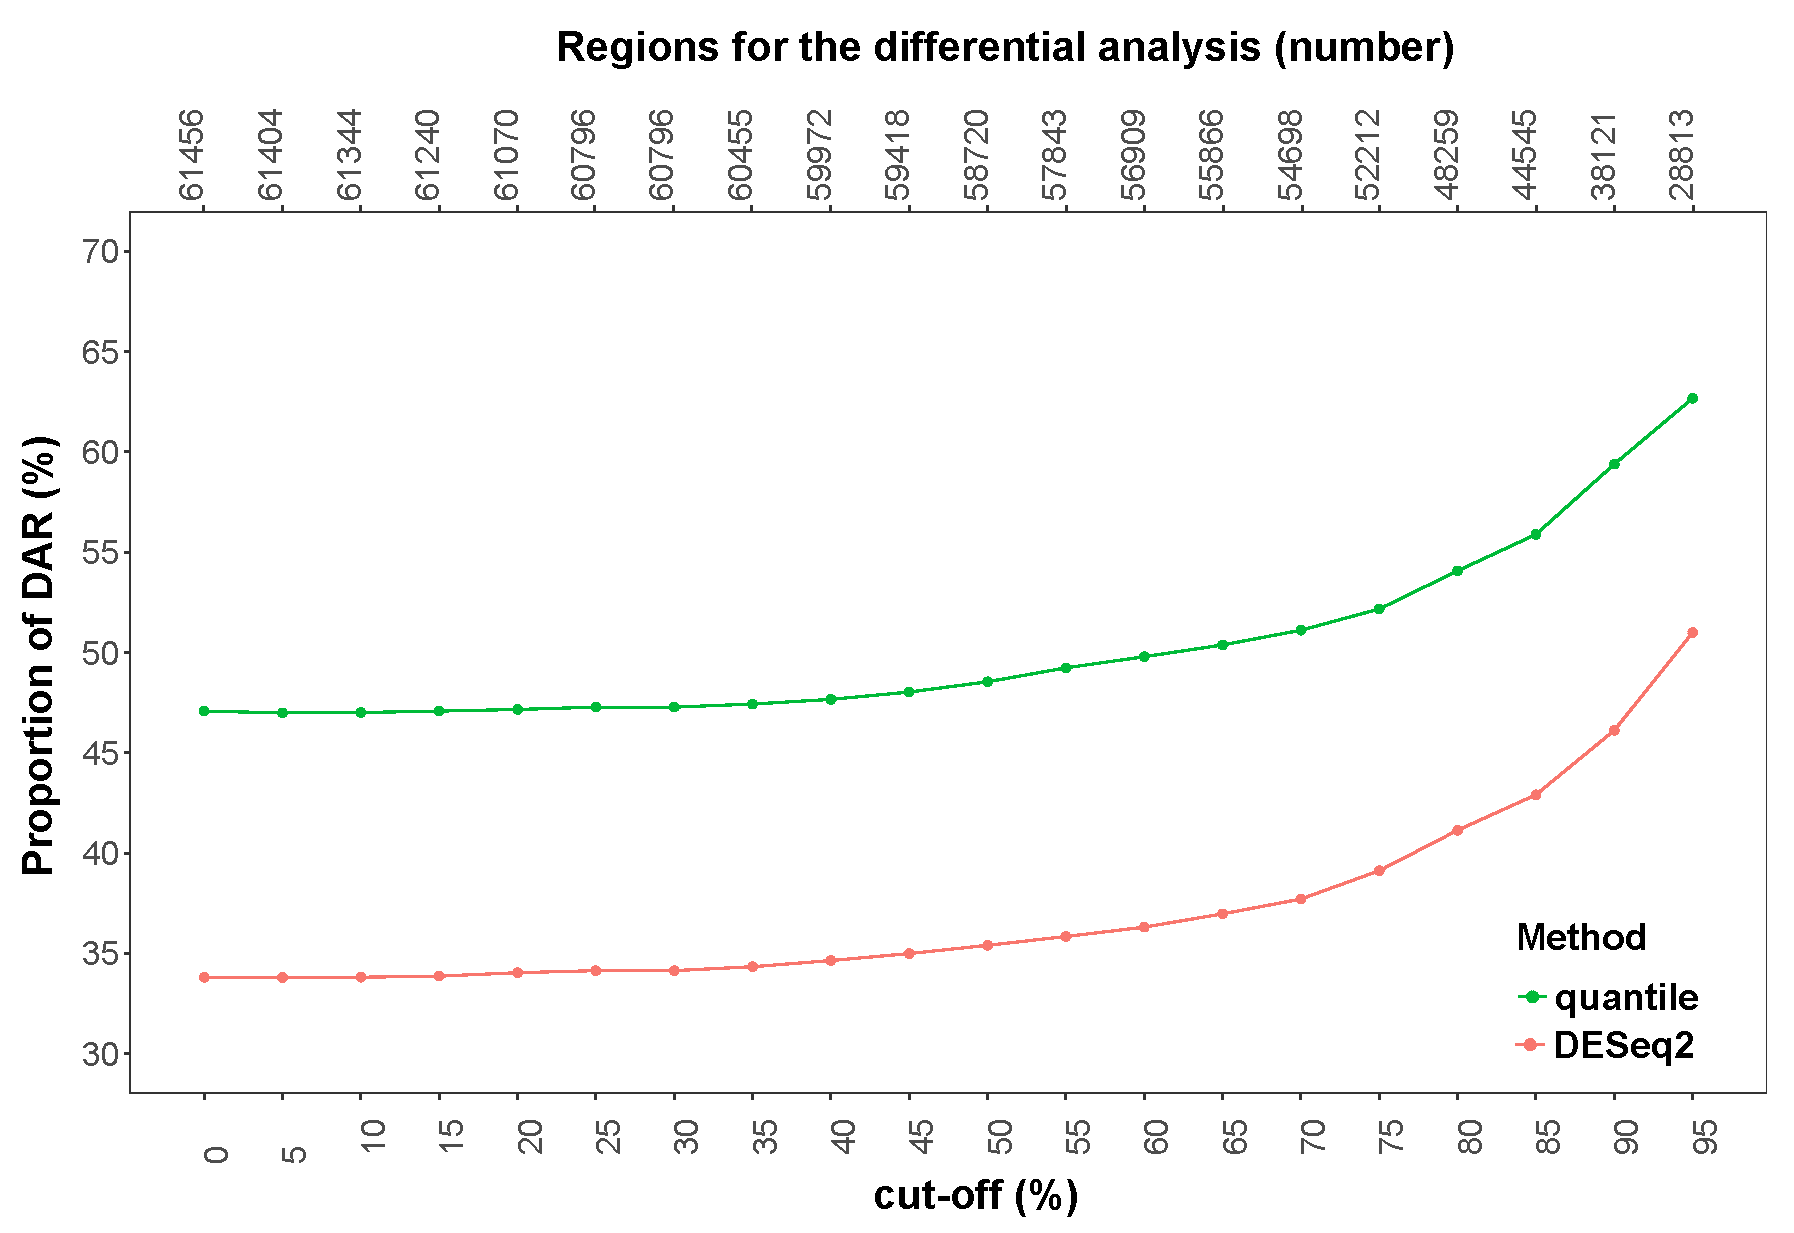
\includegraphics[width=\textwidth]{./Results1/pdfs/ATAC_Core_CD4vsCD14_proportion_DOC_FDR_01_vs_cutoffs_quantile_DESeq2_only}
\caption{\textbf{}}
\end{subfigure}
\begin{subfigure}{0.5\textwidth}
\centering
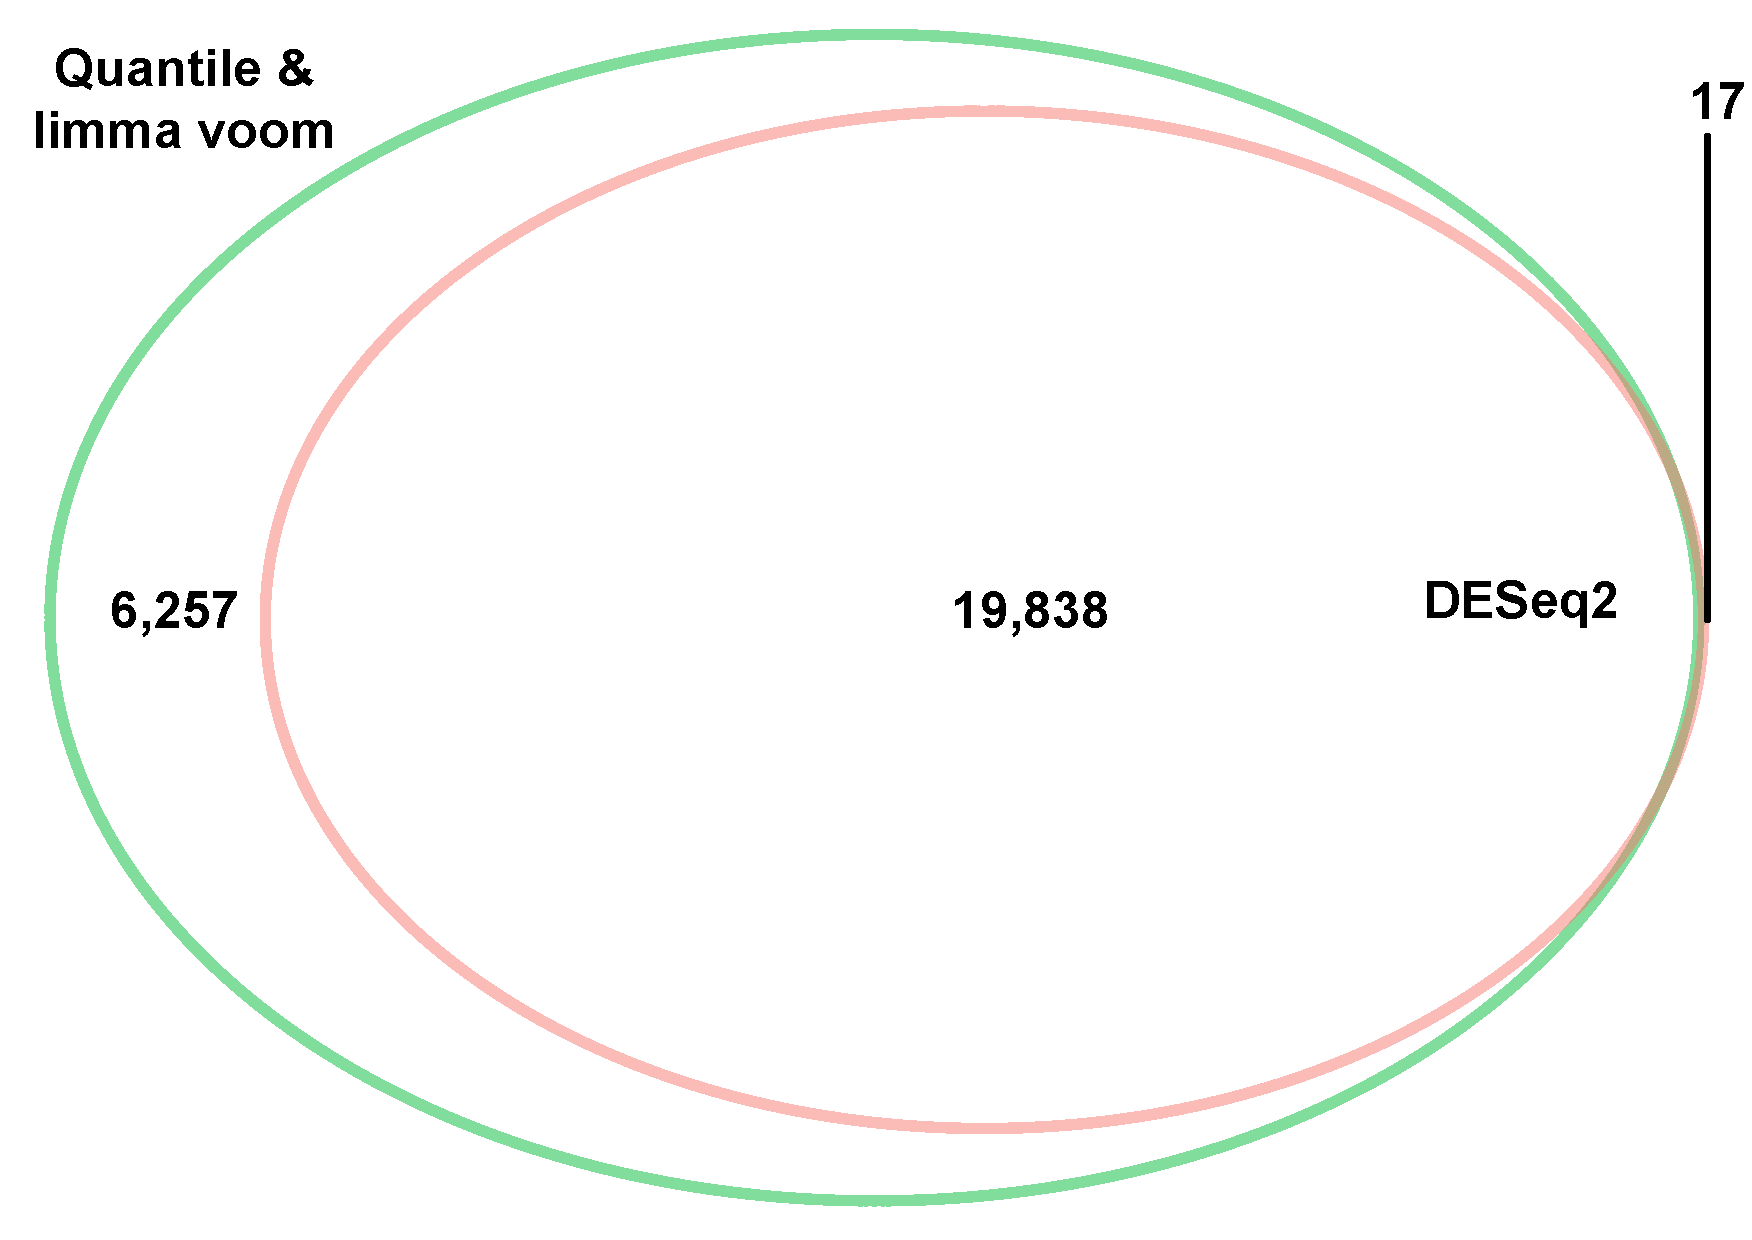
\includegraphics[width=\textwidth]{./Results1/pdfs/ATAC_Core_fresh_CD4vsCD14_venn_diagram_differential_analysis_FDR_01_quantile_DESeq2_only}
\caption{\textbf{}} % to add text to the figure name
\end{subfigure}%
\caption[Differential chromatin accessibility analysis for different background reads cut-offs.]{\textbf{Differential chromatin accessibility analysis using limma voom and DESeq2.\\
}}
\label{fig:DOC_quantile_DESeq2}
\end{figure} 


Both methods performed appropriate normalisation of the counts at each of the master list peaks across the six samples, being the median of the quantile normalisation slightly more consistent across the two cell types compared to DESeq2 (Figure \ref{fig:QC_quantile_DOC_and_DESeq2_comparison} a). When looking at the first FDR ranked 19,855 limma voom DOCs, 18,768 of them were the same as the retrieved by DESeq2. Moreover, very significant positive correlation was found between the fold changed of those 18,768 significant DOCs in both differential analysis methods (r$^2$=0.999, p-val=2.2$^-16$) (Figure \ref{fig:QC_quantile_DOC_and_DESeq2_comparison} b). These observations suggested that the differences in the number of FDR significant DOCs reported by each of the methods could be partly due to differences in the way of calculating the false-positive rate.

 
Clustering and heat map and pathway analysis-briefly


\begin{figure}[htbp]
\centering
\begin{subfigure}{0.48\textwidth}
\centering
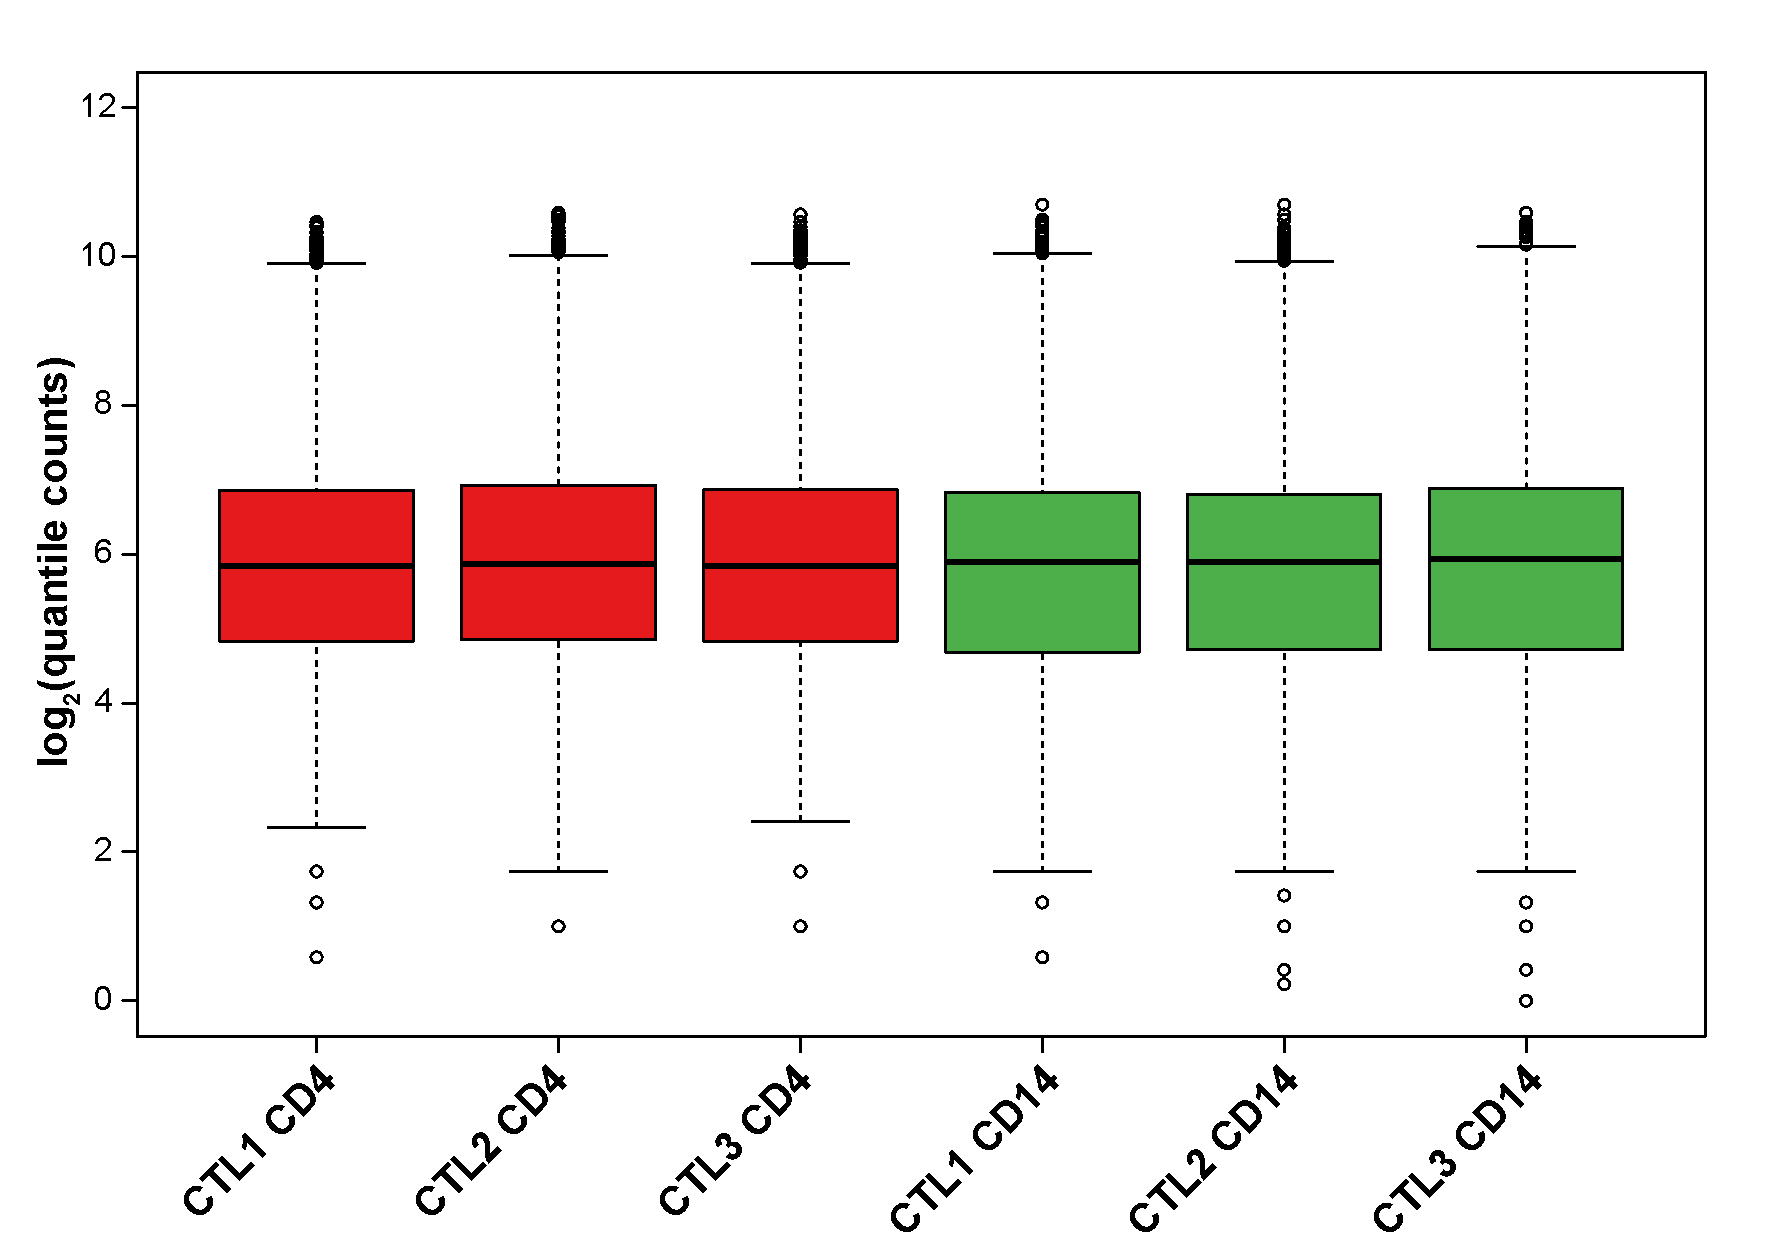
\includegraphics[width=\textwidth]{./Results1/pdfs/ATAC_Core_CD4_CD14_boxplot_80pcnt_cut_off_filtered_quantile_counts}
\caption{\textbf{}}
\end{subfigure}%
\begin{subfigure}{0.48\textwidth}
\centering
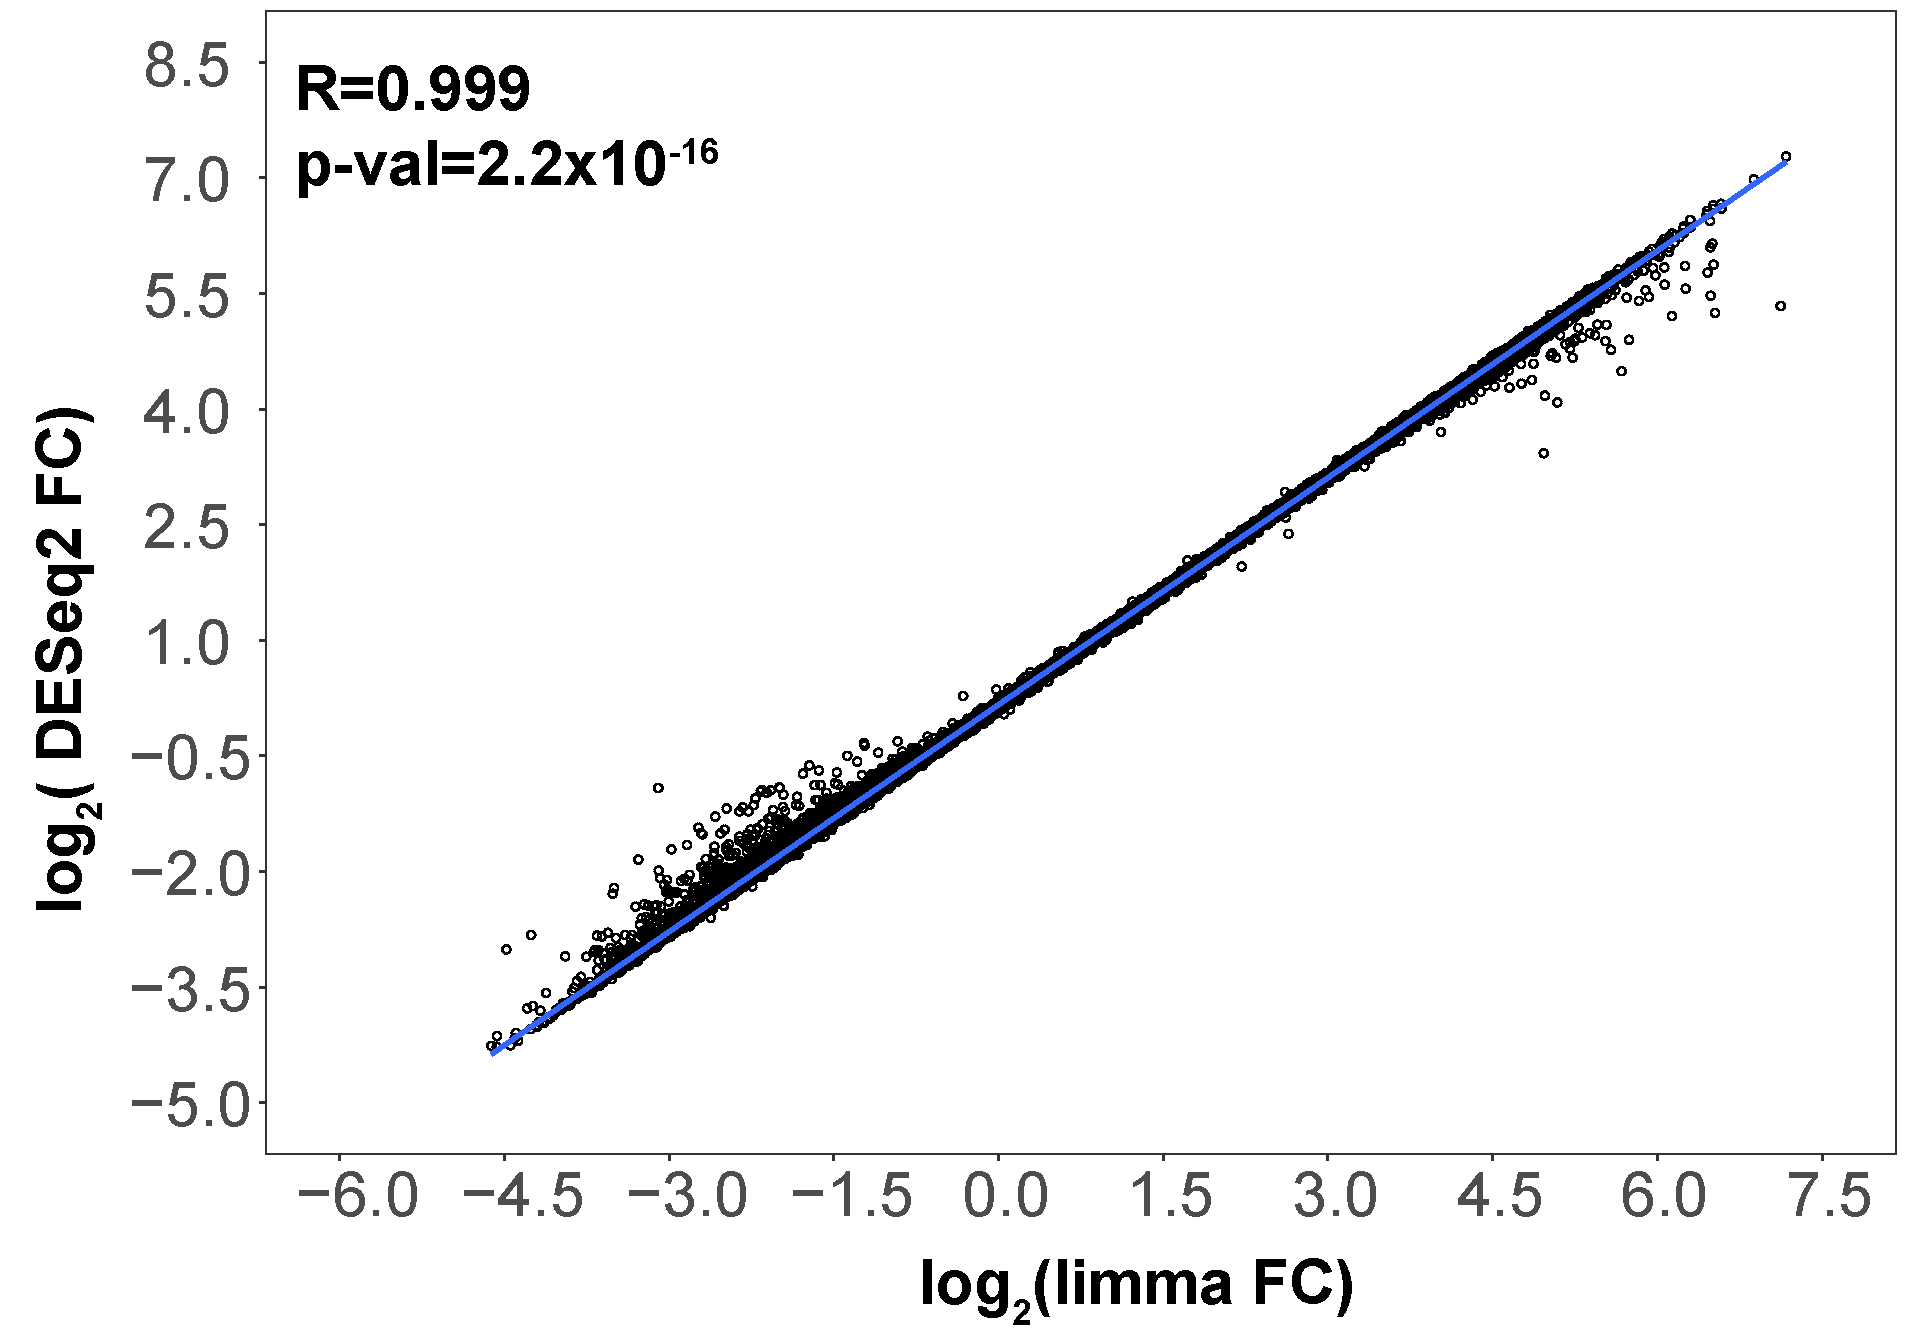
\includegraphics[width=\textwidth]{./Results1/pdfs/ATAC_Core_fastq_CD4_CD14_80pcnt_cut_off_correlation_log2FC_quantile_vs_deseq2}
\caption{\textbf{}}
\end{subfigure}
\begin{subfigure}{0.65\textwidth}
\centering
\includegraphics[width=\textwidth]{./Results1/pdfs/ATAC_Core_CD4vsCD14_clusters_and_heatmap_quantile_common}
\caption{\textbf{}} % to add text to the figure name
\end{subfigure}
\caption[Exploration of the differential chromatin accessibility analysis using 80\% as the empirical cut-off.]{\textbf{Exploration of the differential chromatin accessibility analysis using 80\% as the empirical cut-off.}}
\label{fig:QC_quantile_DOC_and_DESeq2_comparison}
\end{figure} 


\subsection{Assessment of ATAC-seq transposition times and comparison with FAST-ATAC protocol in relevant cell types}


\begin{figure}[htbp]
\centering
\begin{subfigure}{0.5\textwidth}
\centering
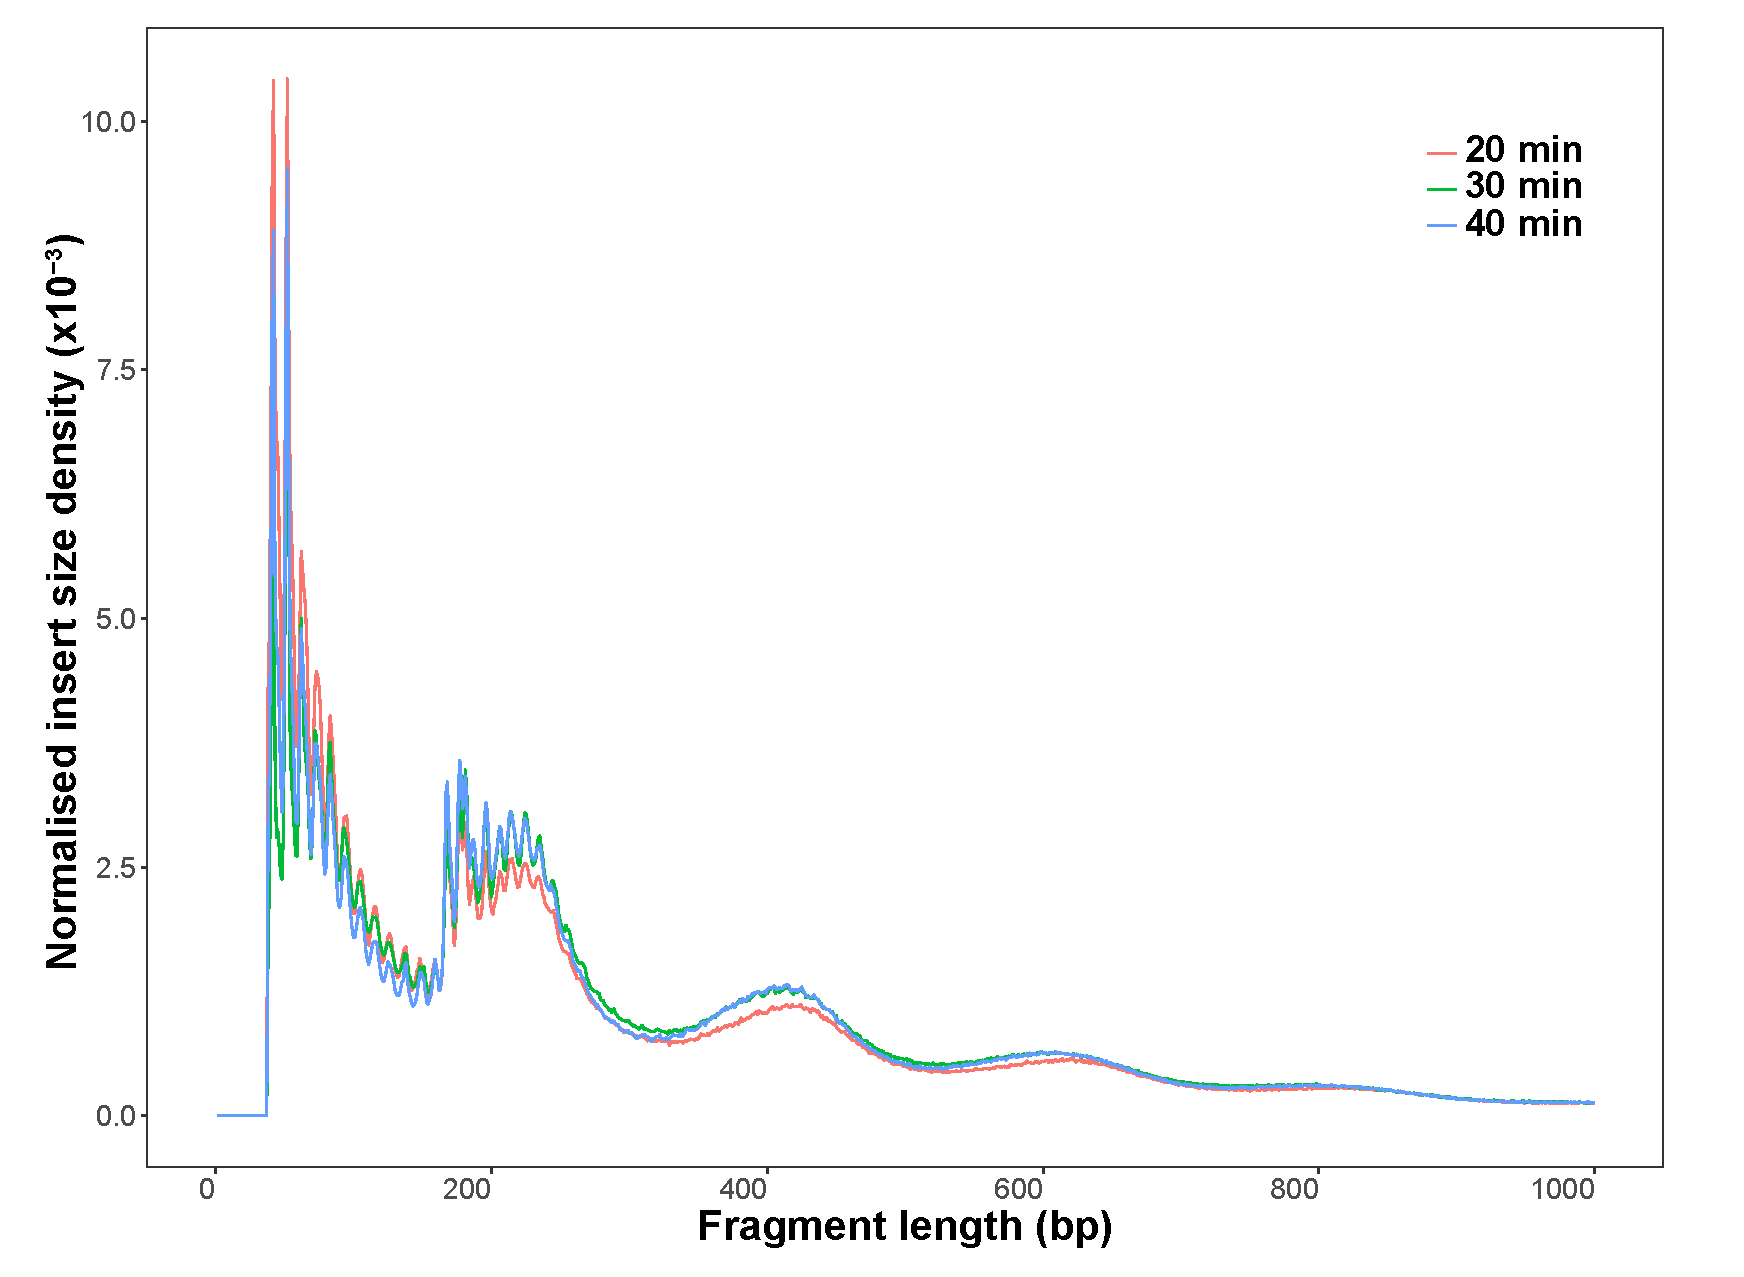
\includegraphics[width=\textwidth]{./Results1/pdfs/ATAC_CD8_fragment_size_distribution_20_30_40min}
\caption{\textbf{}}
% The percentage sign indicated that the other subfig goes side by side
\end{subfigure}
\begin{subfigure}{0.5\textwidth}
\centering
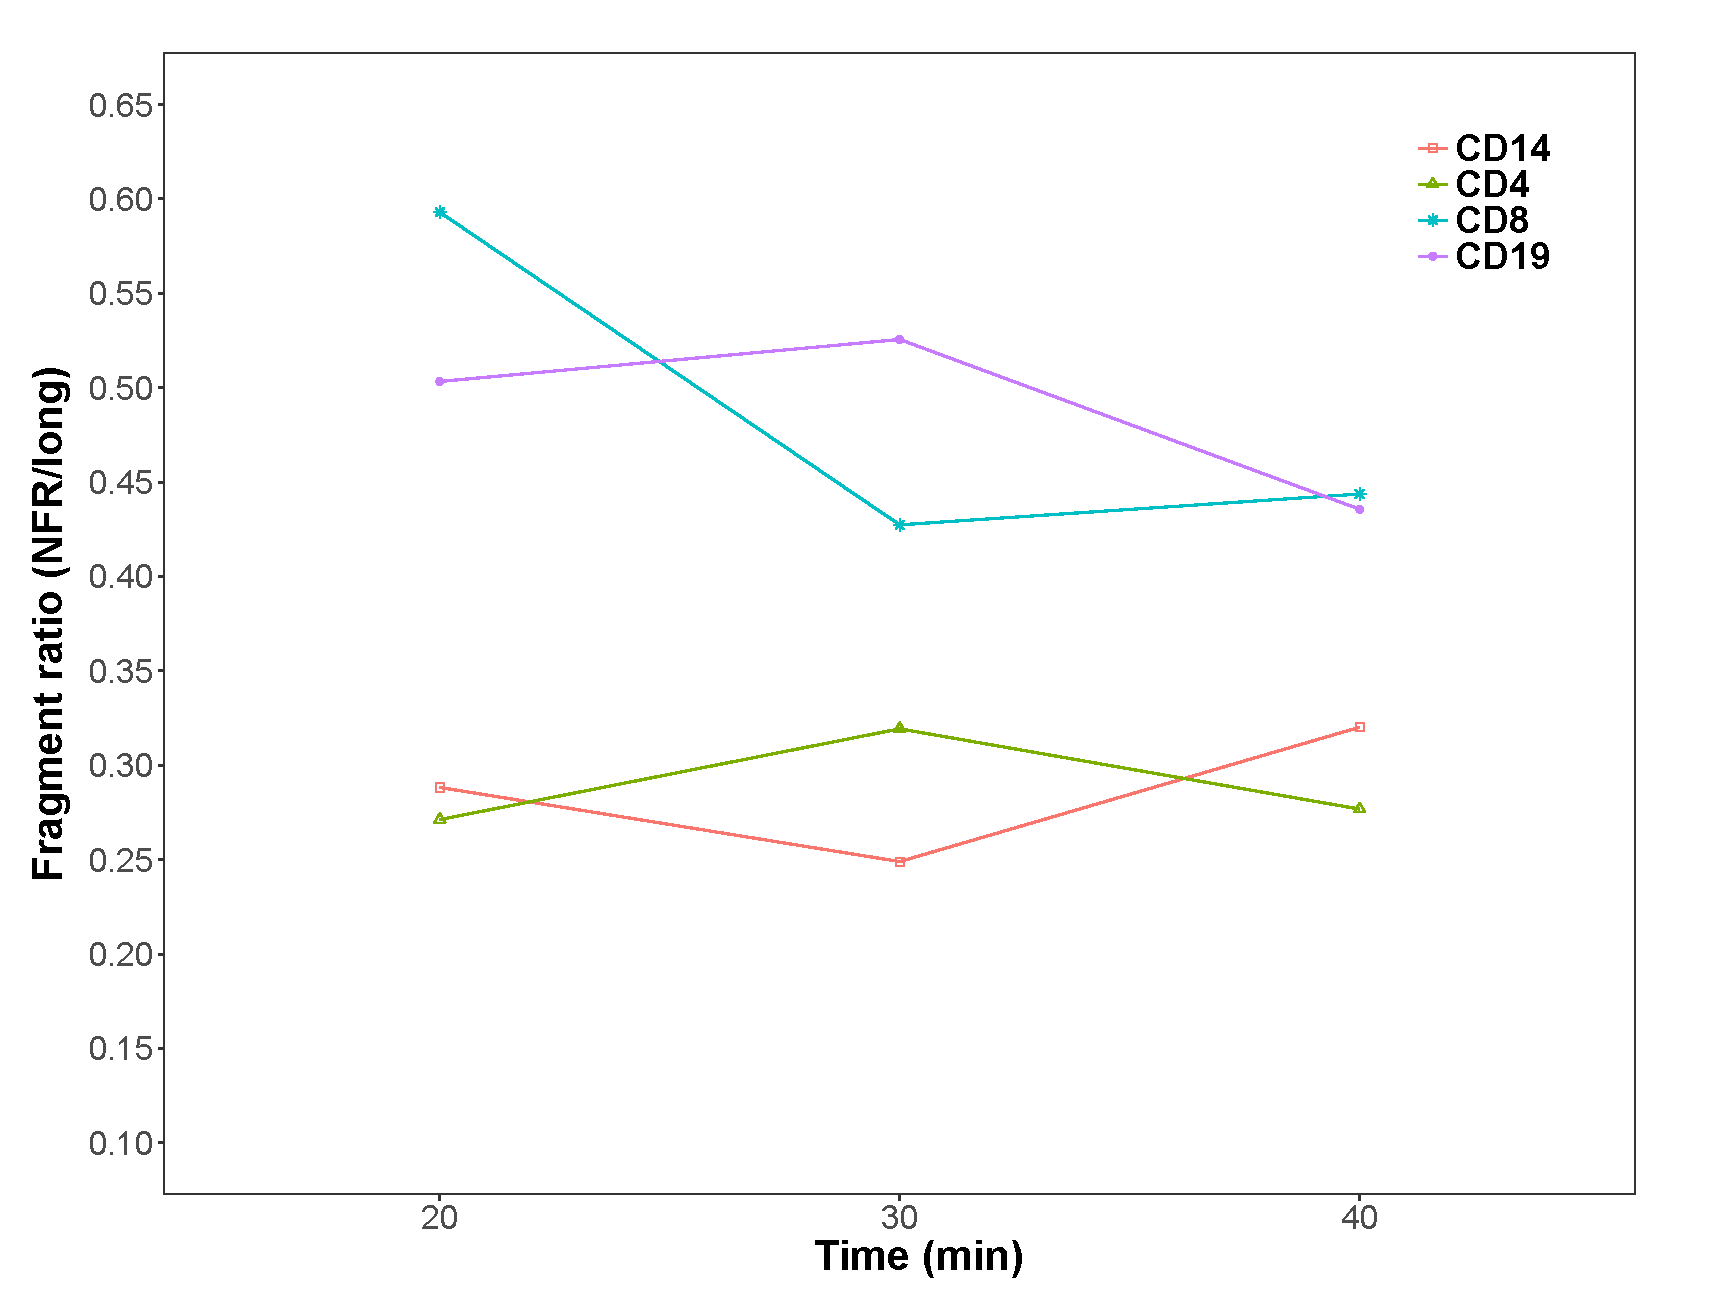
\includegraphics[width=\textwidth]{./Results1/pdfs/ATAC_ratio_short_long_fragments_20_30_40_min}
\caption{\textbf{}}
\end{subfigure} \\
\begin{subfigure}{0.5\textwidth}
\centering
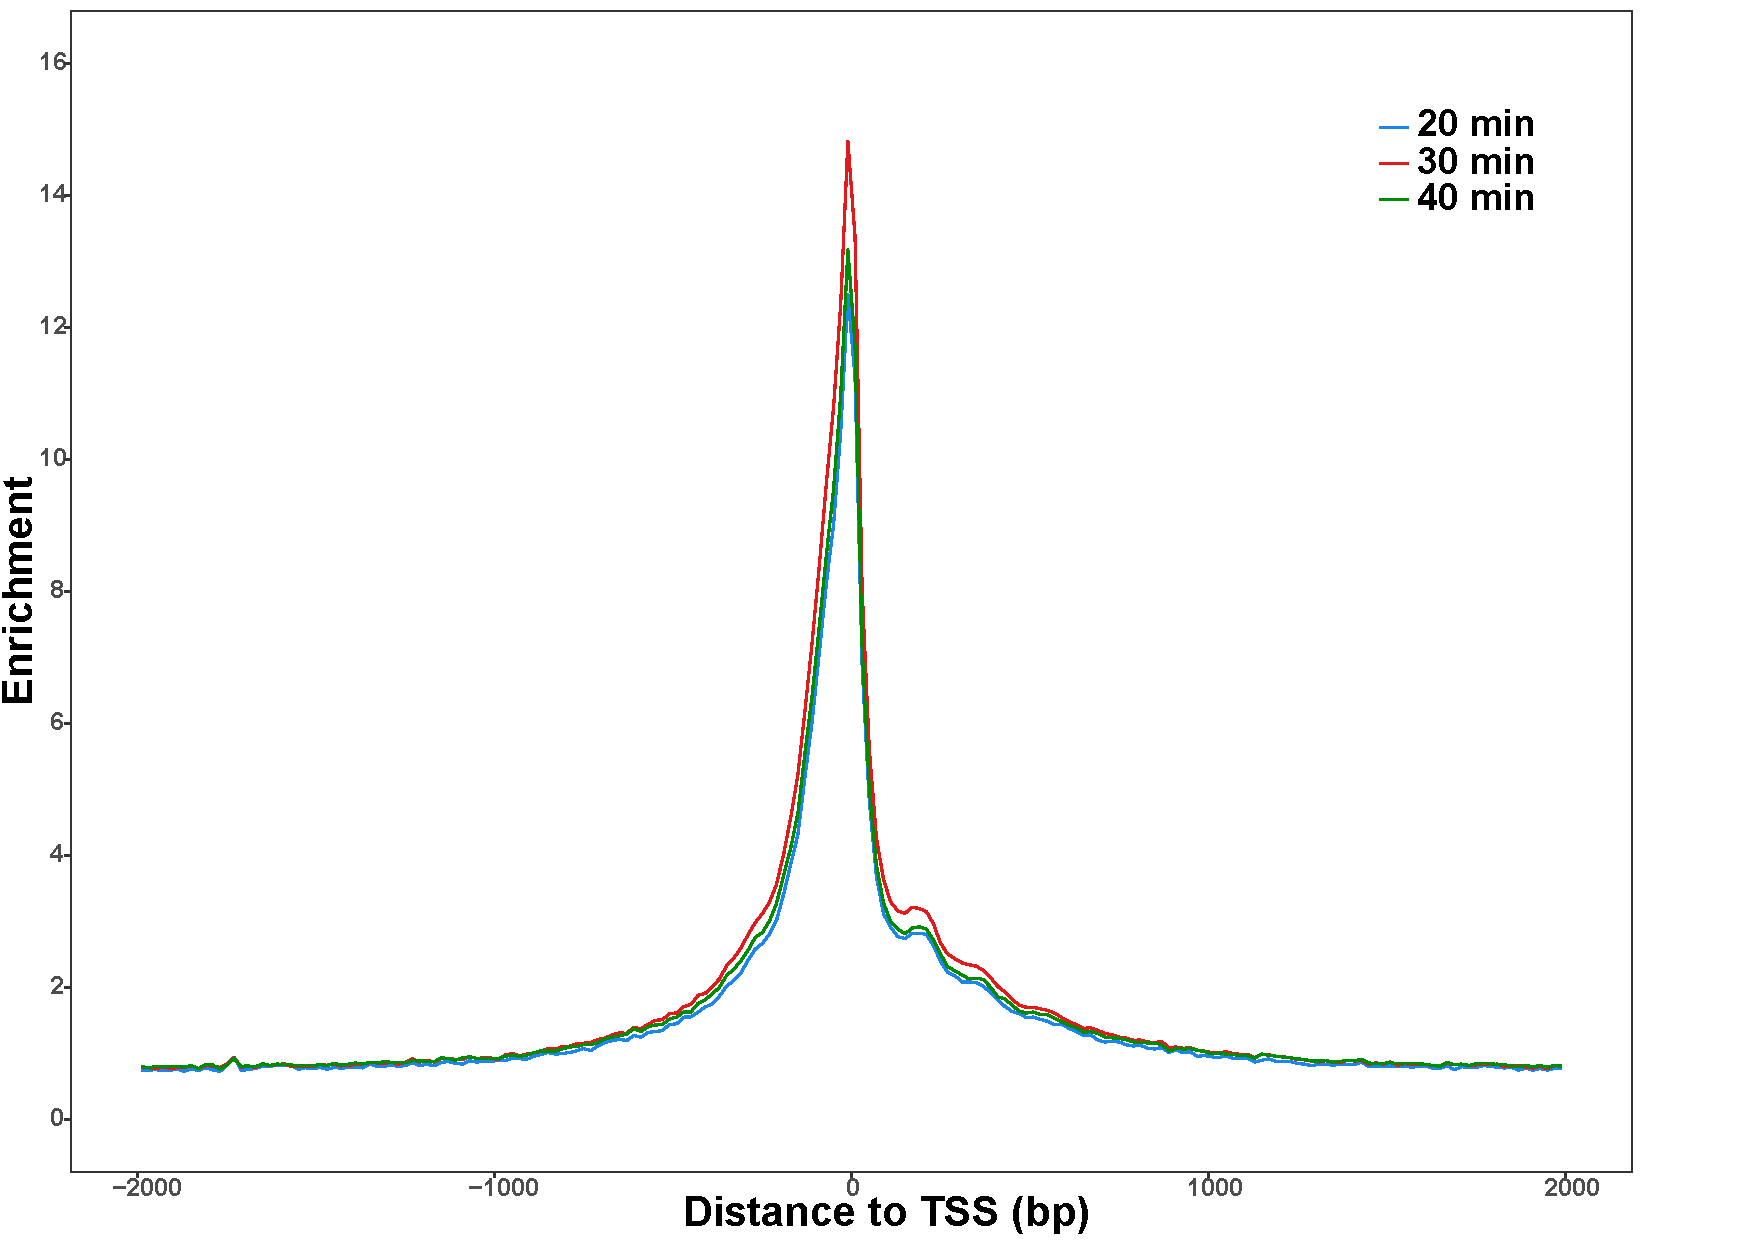
\includegraphics[width=\textwidth]{./Results1/pdfs/ATAC_optimisation_CD4_20_30_40_min_tss_enrichment}
\caption{\textbf{}} % to add text to the figure name
\end{subfigure}
\caption[Assessment of the effect of transposition times on the ATAC-seq QC parameters]{\textbf{Assessment of the effect of transposition times on the ATAC-seq QC parameters} \\
}
\label{fig:Transposition_times_ATAC}
\end{figure} 



\begin{figure}[htbp]
\centering
\begin{subfigure}{0.5\textwidth}
\centering
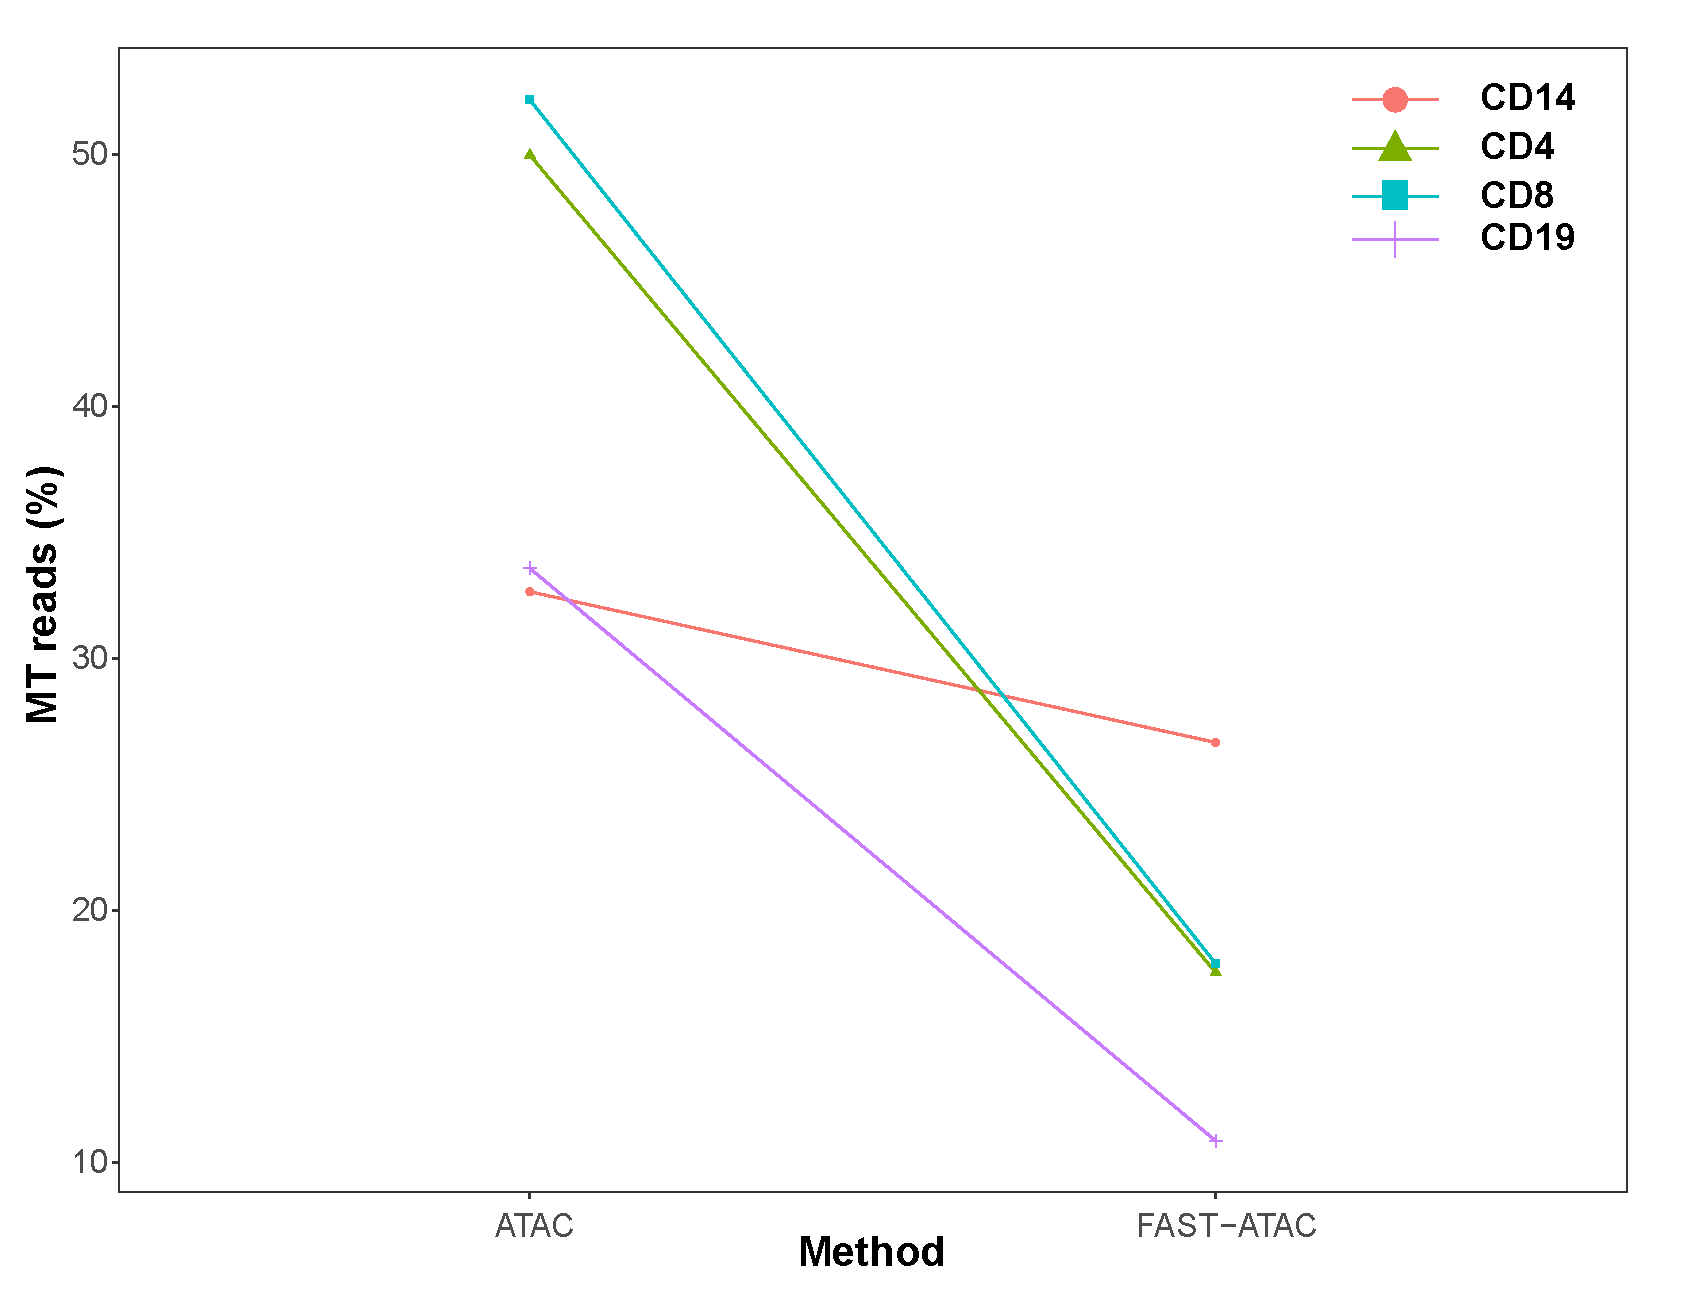
\includegraphics[width=\textwidth]{./Results1/pdfs/ATAC_vs_FAST_ATAC_percnt_MT_reads_dotplot}
\caption{\textbf{}}
% The percentage sign indicated that the other subfig goes side by side
\end{subfigure}%
\begin{subfigure}{0.5\textwidth}
\centering
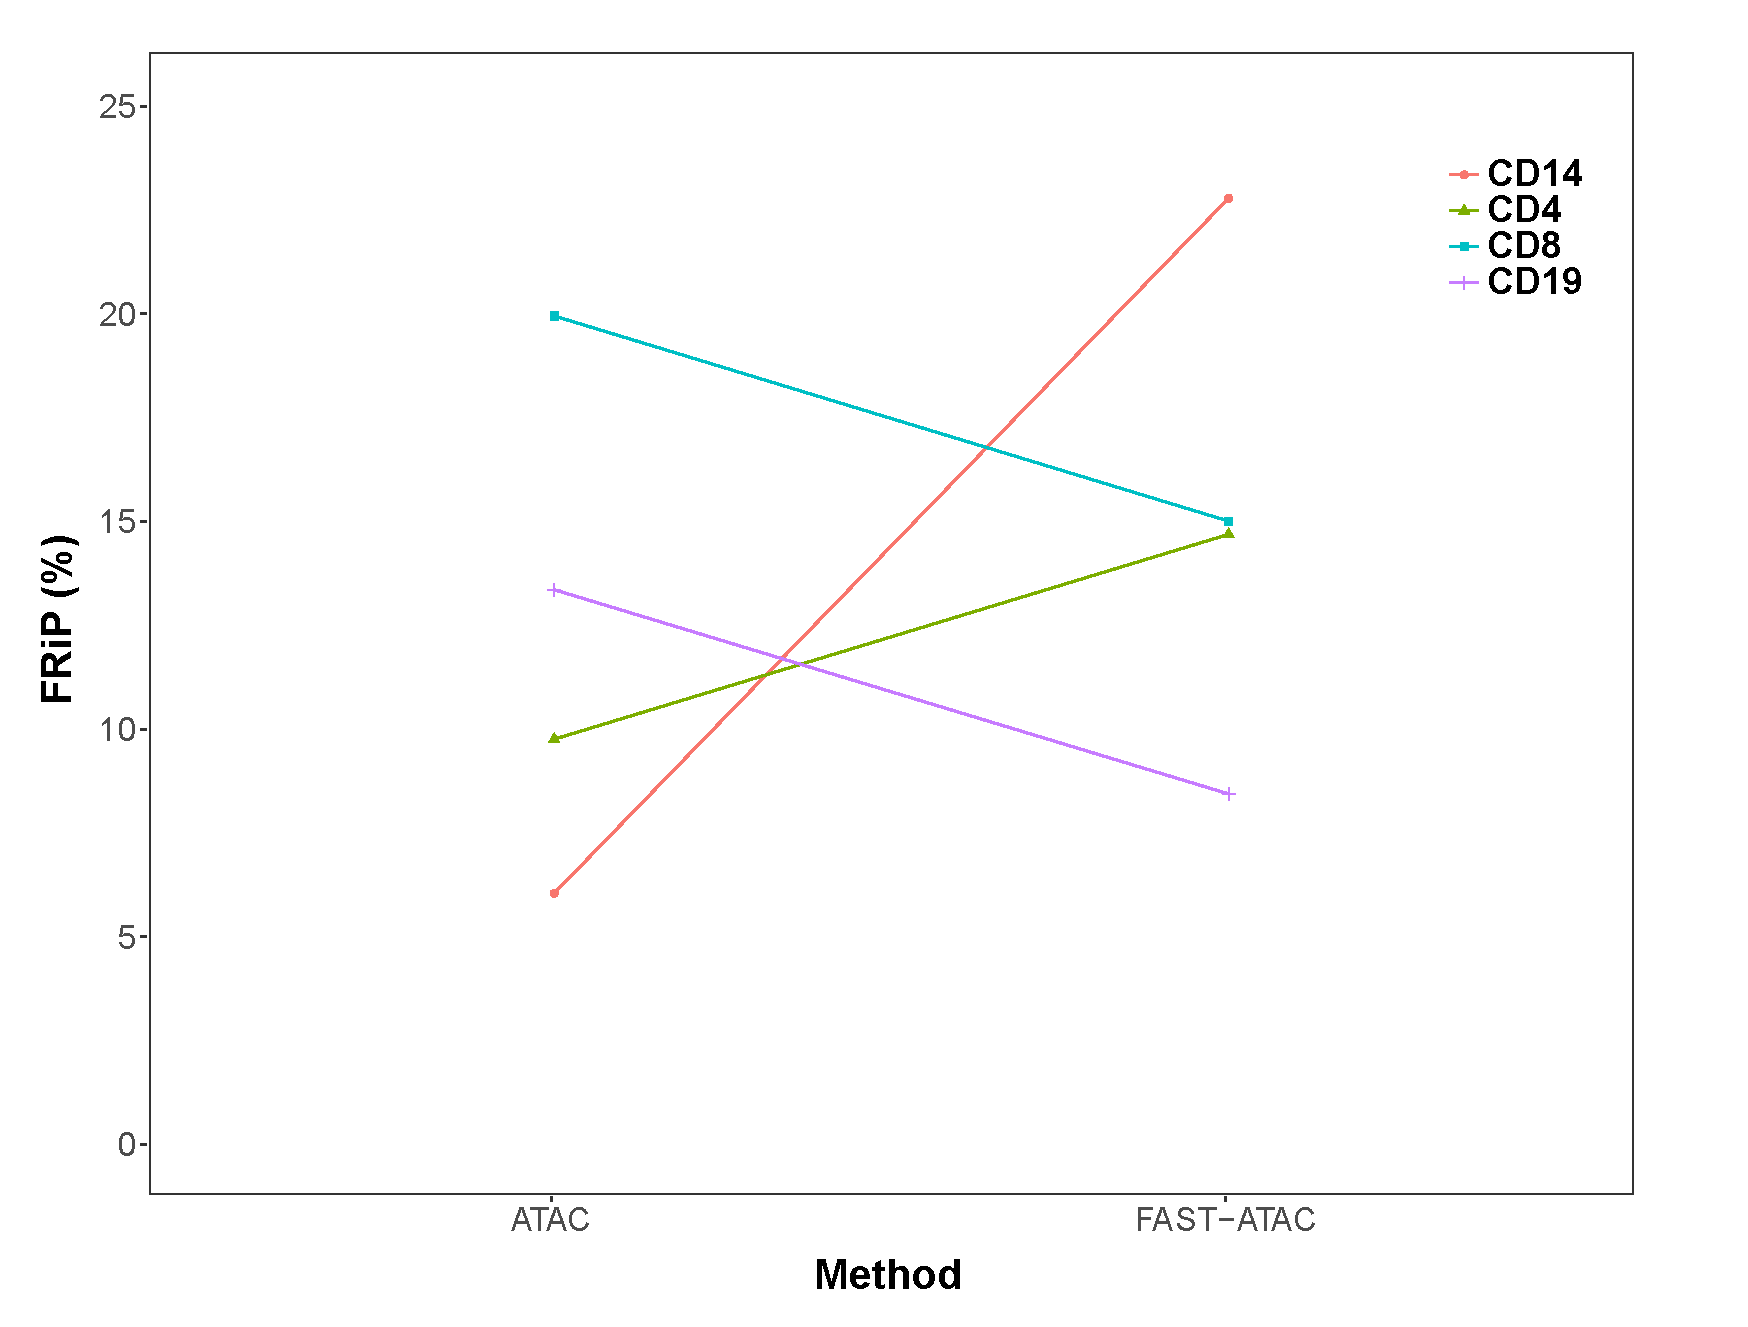
\includegraphics[width=\textwidth]{./Results1/pdfs/ATAC_vs_FAST_ATAC_FRiP_dotplot}
\caption{\textbf{}}
\end{subfigure}
\caption[Differences in MT DNA abundance and signal specificity between ATAC-seq and FAST-ATAC protocols]{\textbf{Differences in MT DNA abundance and signal specificity between ATAC-seq and FAST-ATAC protocols}}
\label{fig:ATAC_vs_FAST_ATAC}
\end{figure} 


\subsection{Impact of cryopreservation and fixation in the chromatin landscape of immune primary cells}
\subsubsection{Experimental design and cohort description}
As previously introduced, research using clinical samples represents a logistic challenge precluding immediate sample processing due to geographical and/or temporal limitations. Therefore long-term storage procedures and the use of preservatives such as fixatives facilitate handling of clinical samples. In the context of these thesis two different approaches were of interest and a collaborative project was established with High-Throughput Genomics at the Wellcome Centre for Human Genomics. On one side, the cryopreservation of PBMCs in liquid nitrogen using DMSO would allow long-term preservation and would require PBMCs thawing and recovery followed by FACS isolation of the cell population of interest. On the other hand, the use of a fixative on the FACS-isolated relevant cell types from the clinical sample could be used as a short term preservation method. Regarding fixative, there was an interest to test the performance of an optimised protocol developed by High-Throughput Genomics using DSP in scRNA-seq \parencite{}. DSP is a cell-permeable and reversible cross-linking fixative that have previously been used to preserve tissue samples for downstream immuno-staining, laser micro-dissection and RNA micro-array expression profiling \parencite{}.

In order to investigate the effect of the cryopreservation and DSP fixation in the nuclear integrity and chromatin structure, three healthy volunteers sex and age matched were processed on different days to be consistent with the case-control experimental design in psoriasis and PsA (Figure \ref{fig:Core_experimental_design}). For each of the individuals PBMCs were isolated from blood and a fraction was stained with the appropriate panel of Abs to isolate CD14$^+$ monocytes and CD4$^+$ T cells, as detailed in Chapter \label{ch:Mat}. ATAC-seq was performed directly in an aliquot of the isolated CD14$^+$ and CD4$^+$ cell. A fraction of the isolated CD14$^+$ and CD4$^+$ cell were appropriately fixed with DPS, stored at 4{$^\circ$}C for 24h and processed for ATAC-seq. A fraction of the PBMCs were cryopreserved following the protocol described in Chapter \label{ch:Mat}, stored in liquid nitrogen for approximately 1 week followed by thawing and recovery in culture for approximately 30 min before undergoing Ab staining and FACS to retrieve CD14$^+$ and CD4$^+$ cells. Altogether, for each of the three controls three matched ATAC-seq samples were generated: ATAC-seq fresh, ATAC-seq fixed and ATAC-seq frozen.


\begin{figure}[H]
\centering
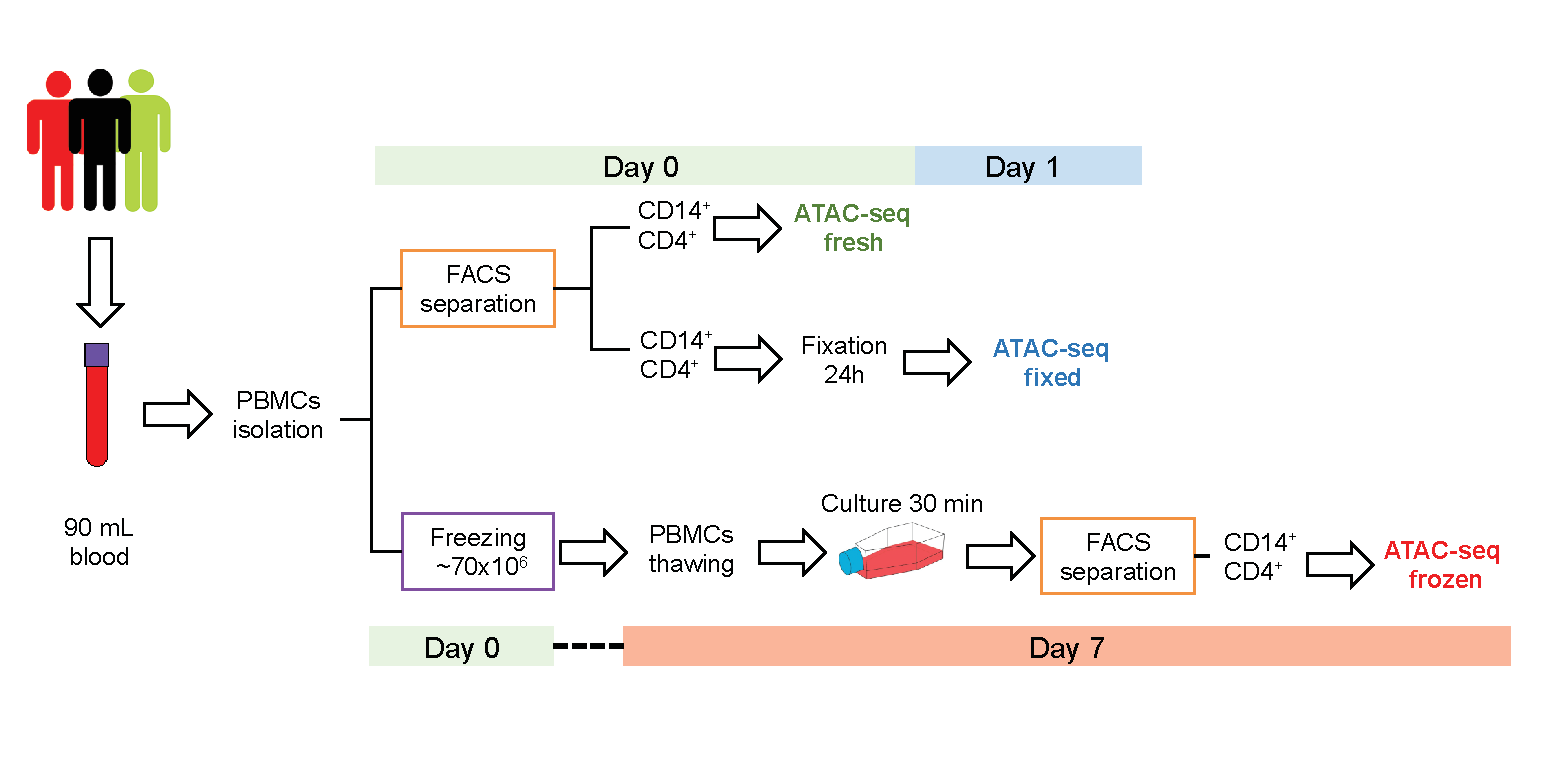
\includegraphics[width=0.7\textwidth]{./Results3/pdfs/Chapter3_core_experimental_design}
\caption[Experimetal design to assess the impact of cryopreservation and fixation in the chromatin accessibility of immune primary cells.]{\textbf{Experimetal design to assess the impact of cryopreservation and fixation in the chromatin accessibility of immune primary cells.}}
\label{figure:Core_experimental_design}
\end{figure}




\subsubsection{Quality control of ATAC-seq data}
\subsubsection{Biological relevance of differentially open chromatin across conditions}




\subsection{Limitations of ATAC-seq and FAST-ATAC to assess chromatin accessibility in KC}

Due to the fact that KC is one of the most relevant cell types in psoriasis pathophysiology, ATAC-seq as described in Buenrostro \textit{et al.}, 2013 (named as ATAC-seq 1 here) was performed in 50,000 cells of a suspensions isolated from a psoriasis lesional skin biopsy. Two different tranposition times (30 and 40 min) where tested. Since biopsy handling and lesional epidermal KC are particularly challenging this was considered the best system to test the performance of the standard protocol in the clinical setting of interest for the study. Two tranposition times (30 and 40 min) where tested.


\begin{figure}[htbp]
\centering
\begin{subfigure}{0.65\textwidth}
\centering
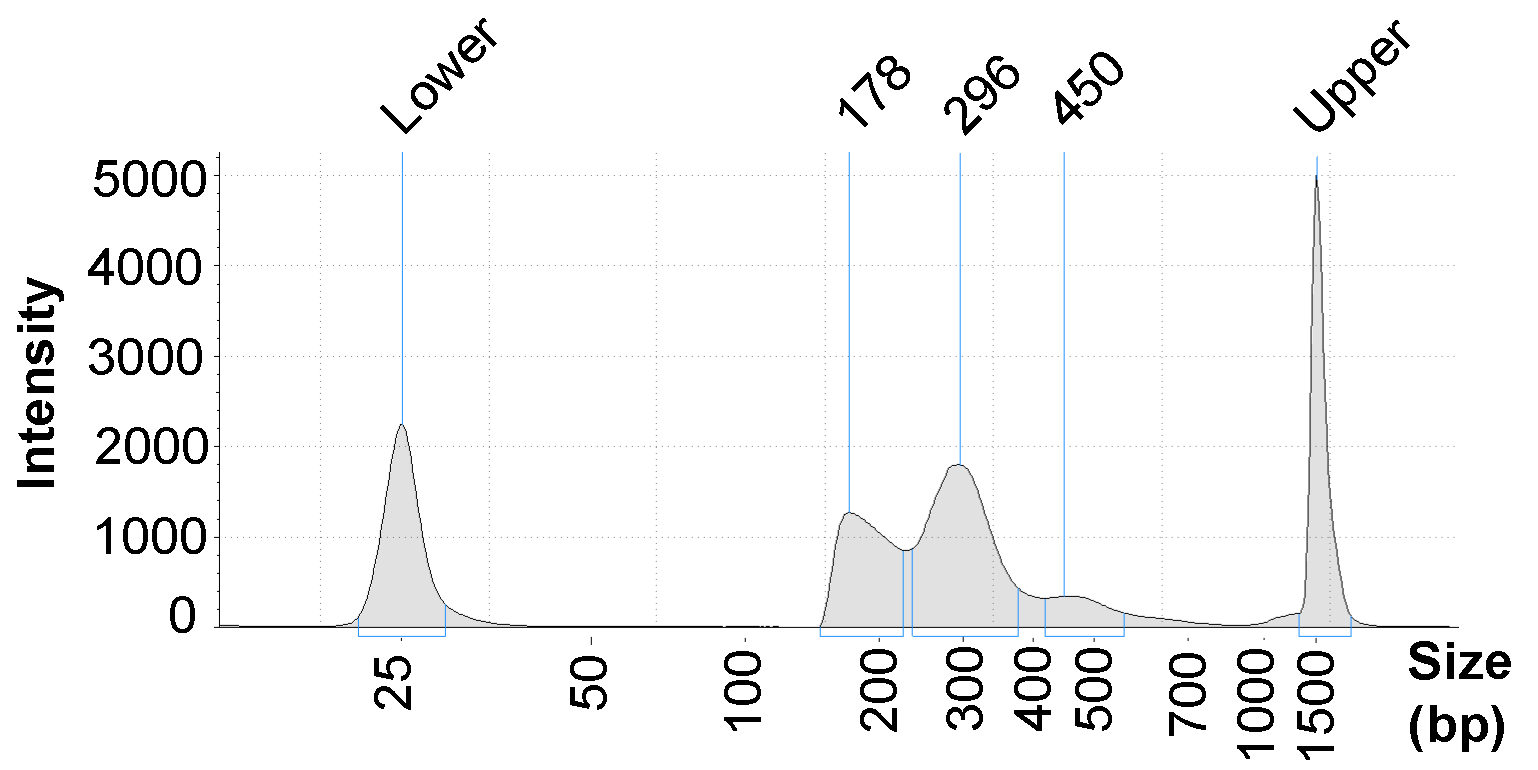
\includegraphics[width=\textwidth]{./Results1/pdfs/ATAC_PS02_tapestation_30min}
\caption{\textbf{}}
\end{subfigure}
\begin{subfigure}{0.45\textwidth}
\centering
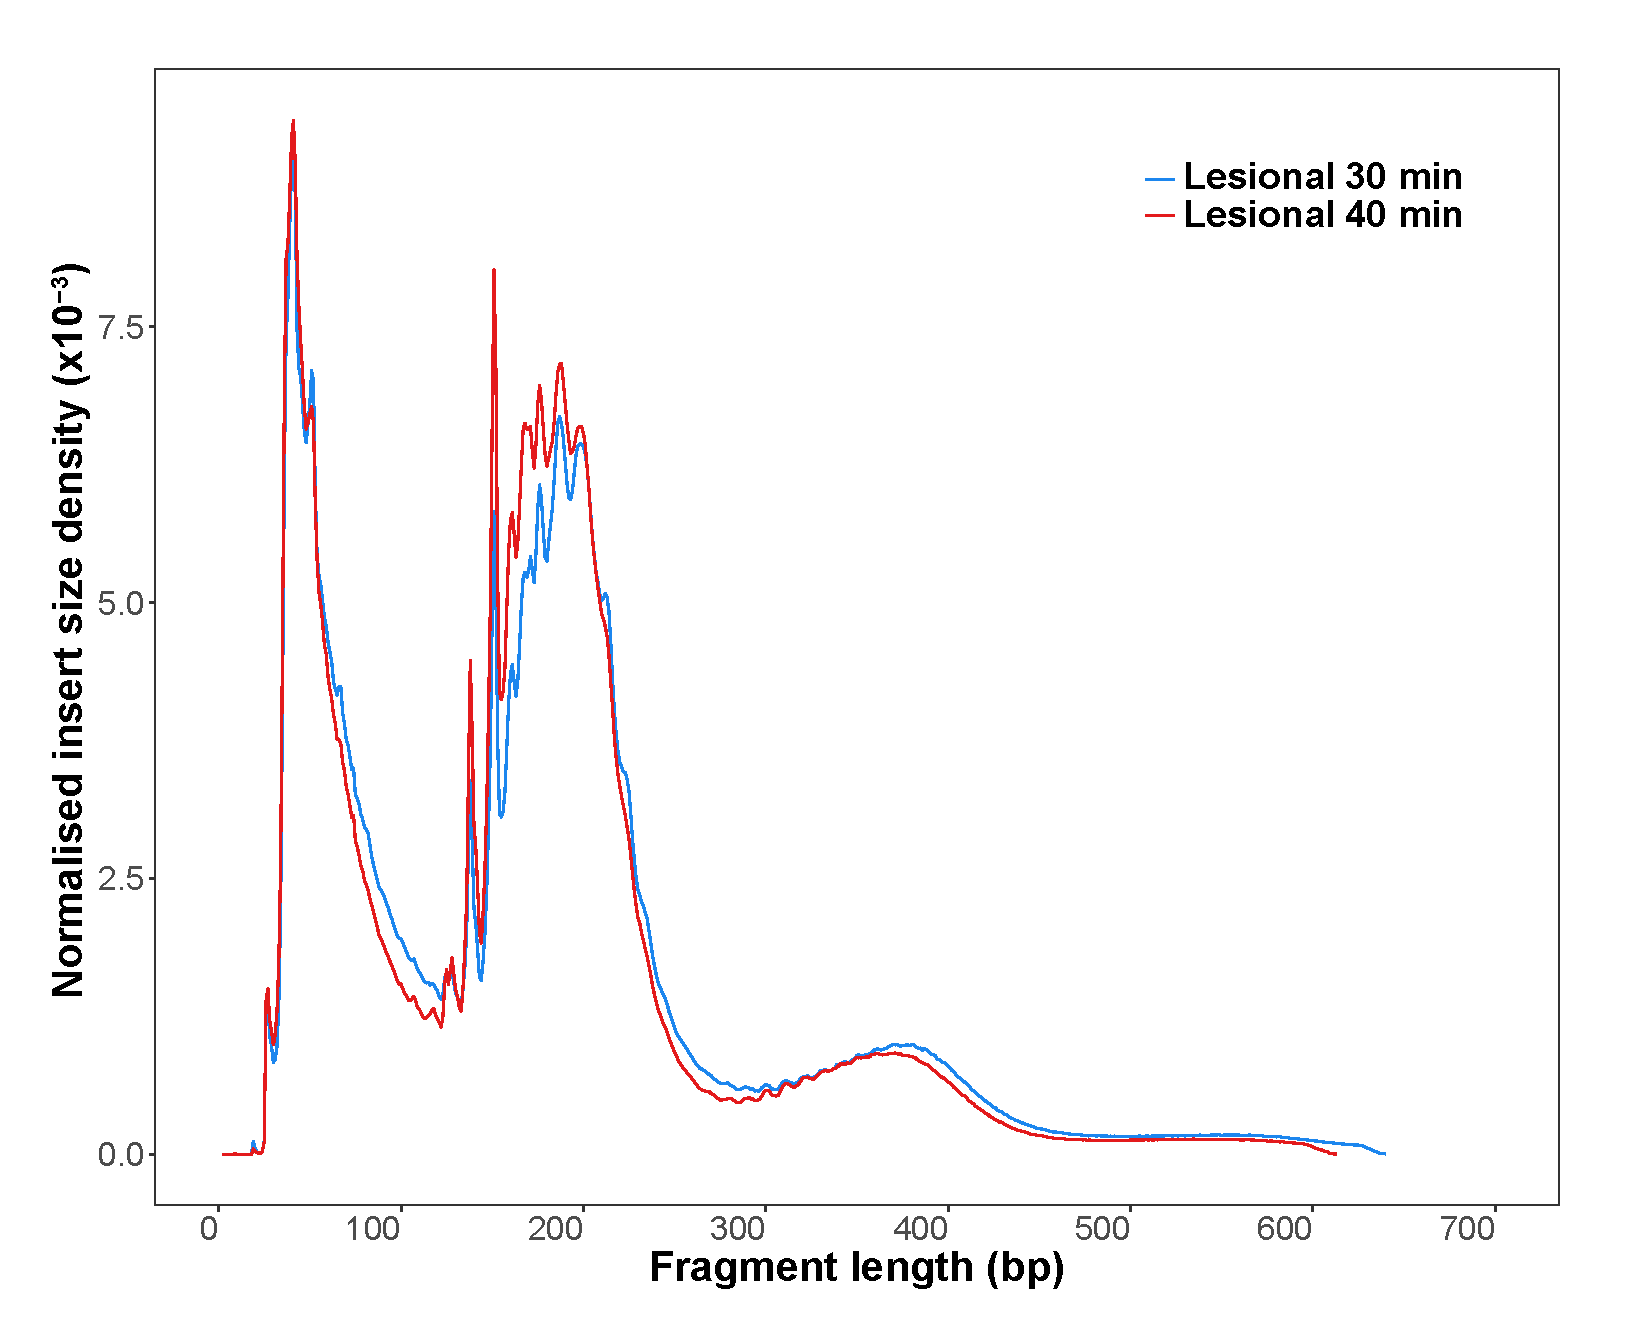
\includegraphics[width=\textwidth]{./Results1/pdfs/ATAC_PS-2_30_40_min_fragment_size_distribution}
\caption{\textbf{}}
\end{subfigure}%
\begin{subfigure}{0.45\textwidth}
\centering
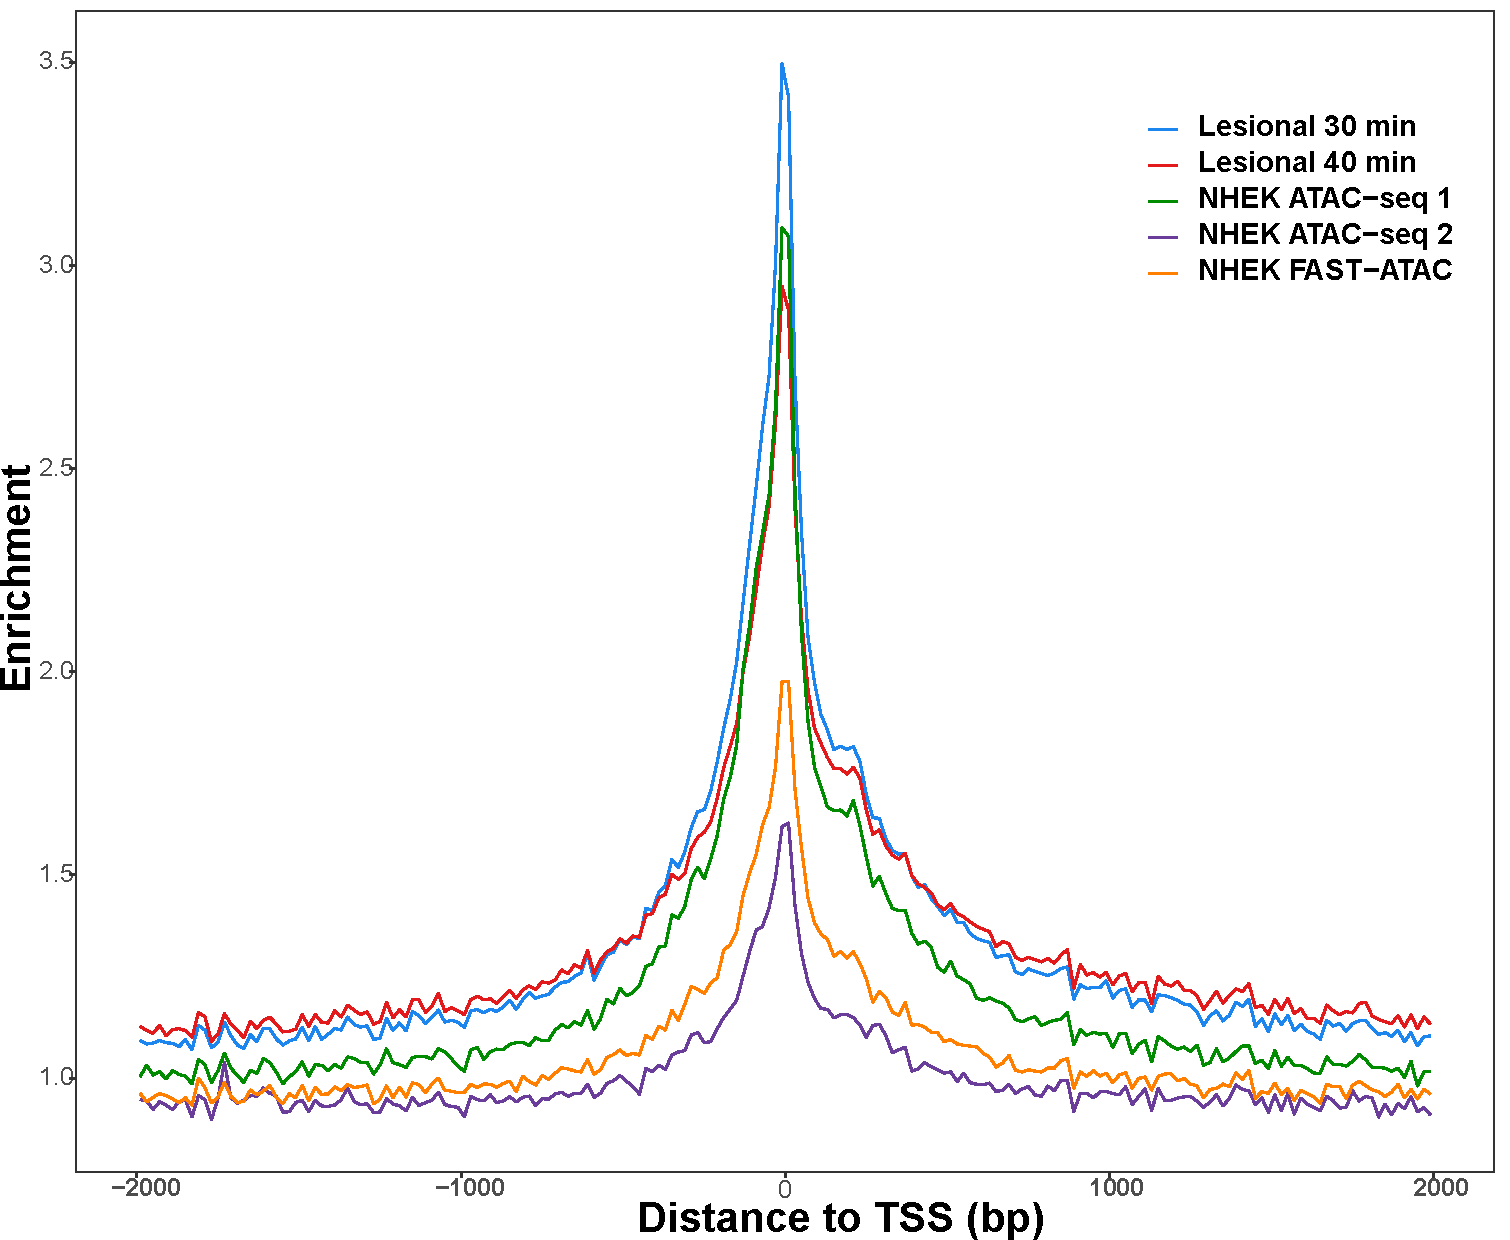
\includegraphics[width=\textwidth]{./Results1/pdfs/ATAC_skin_TSS_enrichment_PS02_30_40min_NHEK_ATAC1_ATAC_2_FAST_ATAC}
\caption{\textbf{}} % to add text to the figure name
\end{subfigure}
\caption[QC assessment of ATAC-seq in KC enriched cell suspension derived from a psoriatic lesional skin biopsy]{\textbf{QC assessment of ATAC-seq in KC enriched cell suspension derived from a psoriatic lesional skin biopsy}. Two transposition times (30 and 40 min) were tested using the standard ATAC-seq protocol (Buenrostro \textit{et al.}, 2013 in 50,000 cells from the same suspension.}
\label{fig:PS02_skin_ATAC_QC_assessment}
\end{figure} 




Although cell suspension obtained from biopsies using trypsinisation of the epidermal sheet are 90\% enriched in KC, they also contain significant amounts of dead cells and free-DNA releases by apoptotic cells. In order to overcome this problem and the impact that it may have over ATAC-seq background signal, viable KC were selected by adherence assay. Biopsy cell suspensions were cultured for 3h in a 96-well plate and washed afterwards to ensure that only the viable and less differentiated KC would remain for down stream analysis. In parallel cultured NHEK were also used to assess the performance of the different ATAC-seq protocols.

Table for the conditions: done
Tapestation profiles of the the chosen condition. done Send the others to supplementary.
QC measurements: for ATAC1, ATAC2 and NHEK, mention frag size distribution done
DHS enrichment for p and q done but not convincing.The complex network of keratin filaments in stratified epithelia is tightly regulated during squamous cell differentiation. Keratin 14 (K14) is expressed in mitotically active basal layer cells, along with its partner keratin 5(K5), and their expression is down-regulated as cells differentiate.


\begin{table}[htbp]
%\setlength{\tabcolsep}{20pt}
%\renewcommand{\arraystretch}{1.5}
\begin{tabular}{@{} c c c}
\toprule
\textbf{Protocol} & \textbf{Lysis and} & \textbf{Key parameters} \\
                  & \textbf{transposition} &  \\
\midrule
\midrule
Buenrostro \texit{et al.,} 2013 & Two steps & 0.1\% NP-40 and 2.5$\micro$L Tn5  \\
&&&
Bao \texit{et al.,} 2015        &Two steps   & 0.05\% NP-40 and 5$\micro$L Tn5  \\
&&&
                                &          & C1: 0.01\% digitonin, 0.5$\micro$L Tn5 \\
                                &          & C2: 0.01\% digitonin, 2.5$\micro$L Tn5 \\
 Corces \texit{et al.,} 2016    & One step & C3: 0.025\% digitonin, 0.5$\micro$L Tn5 \\
													      &          & C4: 0.025\% digitonin, 2.5 $\micro$L Tn5 \\
\bottomrule
\end{tabular}
\medskip %gap
\caption[Description of the most relevant parameter from the ATAC-seq and FAST-ATAC protocols assayed in NHEK and skin biopsies.]{\textbf{ Description of the most relevant parameter from the ATAC-seq and FAST-ATAC protocols assayed in NHEK and skin biopsies.}Transposition for all the different protocols was 30 min.}
\label{tab:ATAC_skin_optimisation_protocols}
\end{table}
\bigskip %bigger space



\begin{figure}[htbp]
\centering
\begin{subfigure}{0.48\textwidth}
\centering
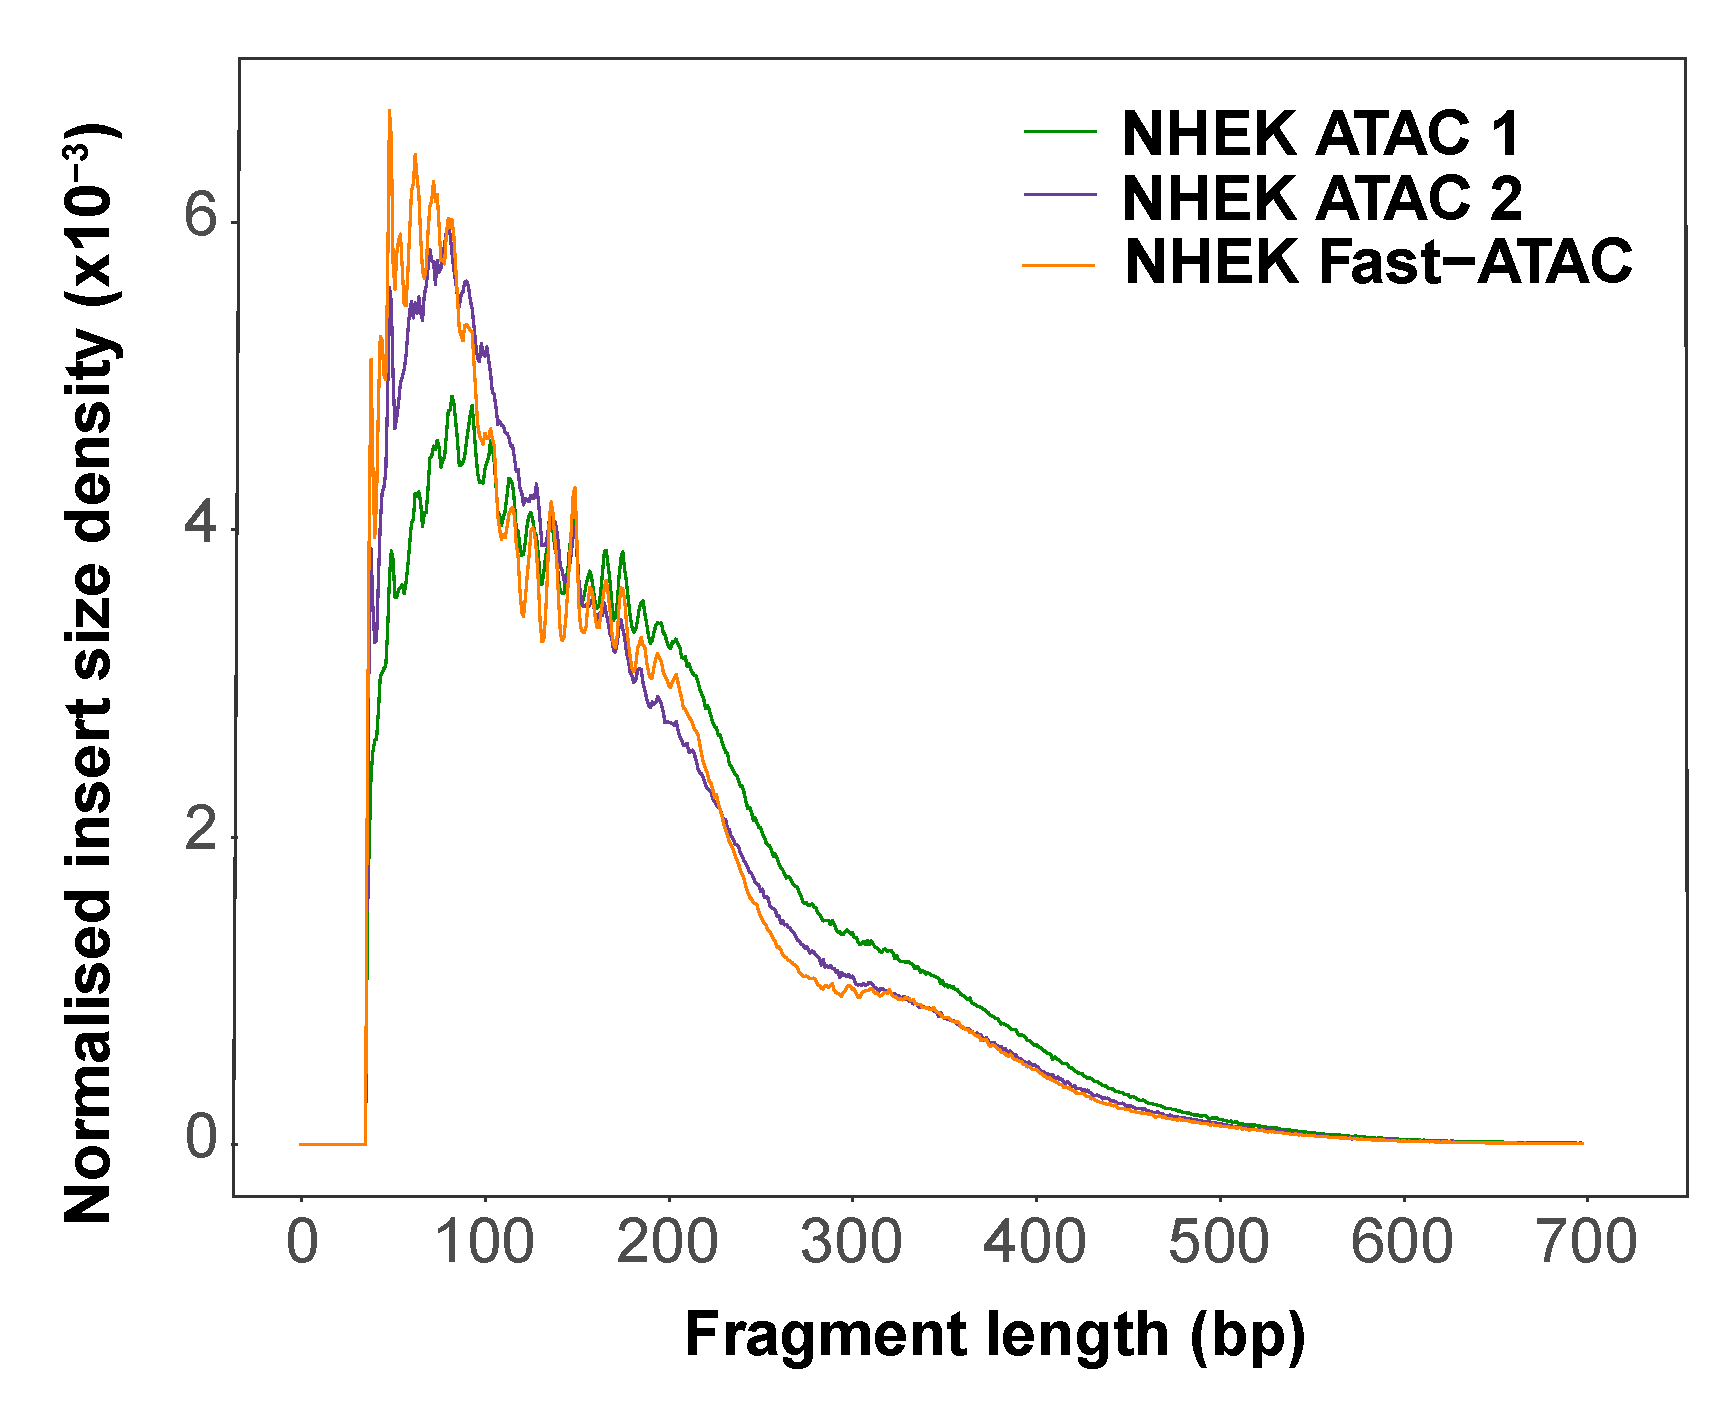
\includegraphics[width=\textwidth]{./Results1/pdfs/ATAC_NHEK_ATAC1_ATAC2_FAST_ATAC_fragment_size_distribution}
\caption{\textbf{}}
\end{subfigure}%
\begin{subfigure}{0.48\textwidth}
\centering
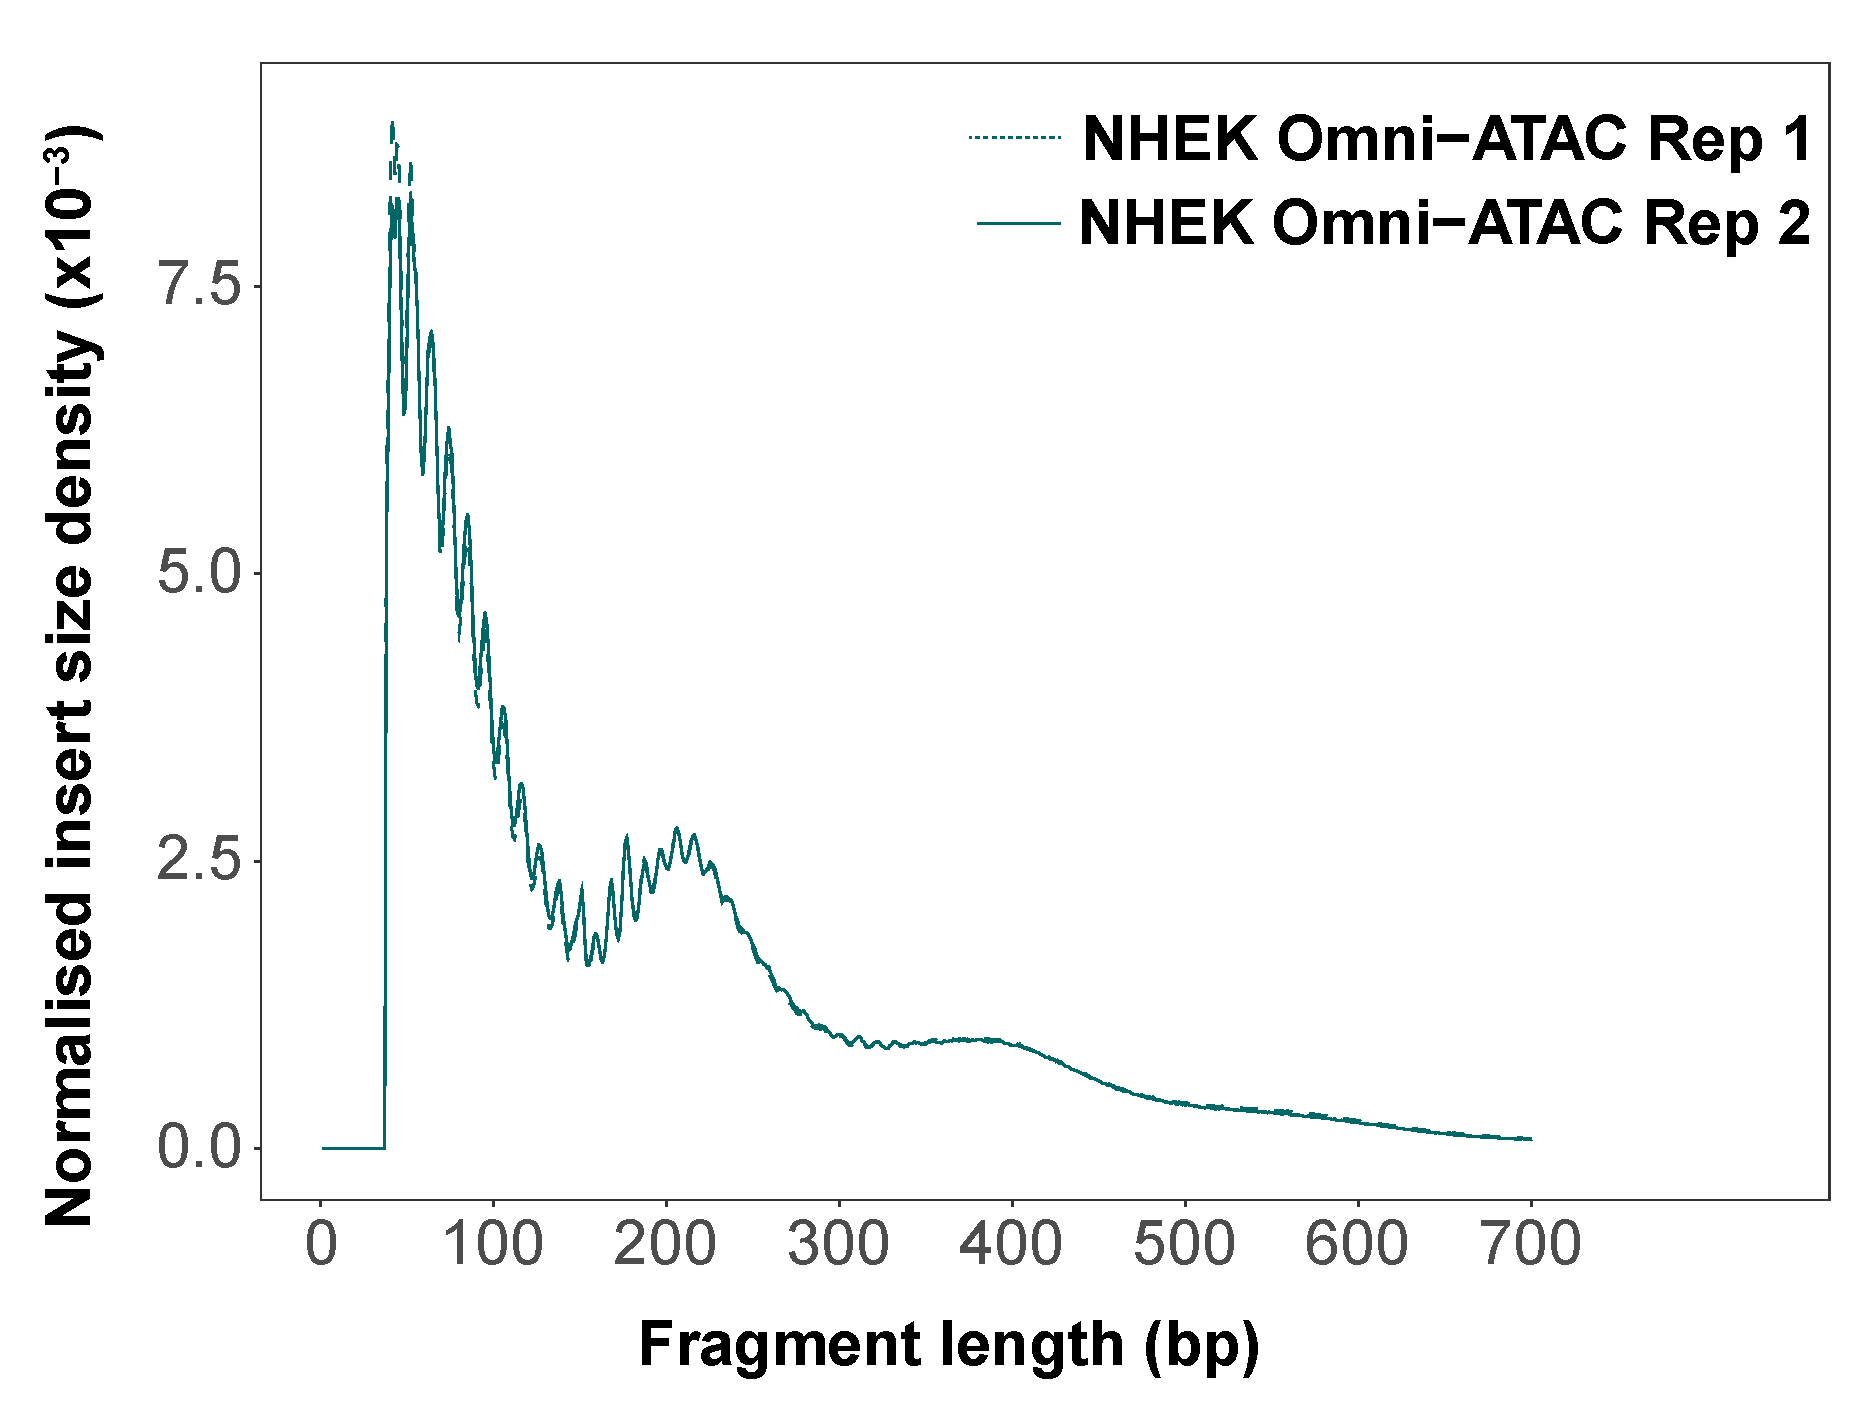
\includegraphics[width=\textwidth]{./Results1/pdfs/ATAC_NHEK_Omni_ATAC_fragment_size_distribution}
\caption{\textbf{}}
\end{subfigure}
\begin{subfigure}{0.5\textwidth}
\centering
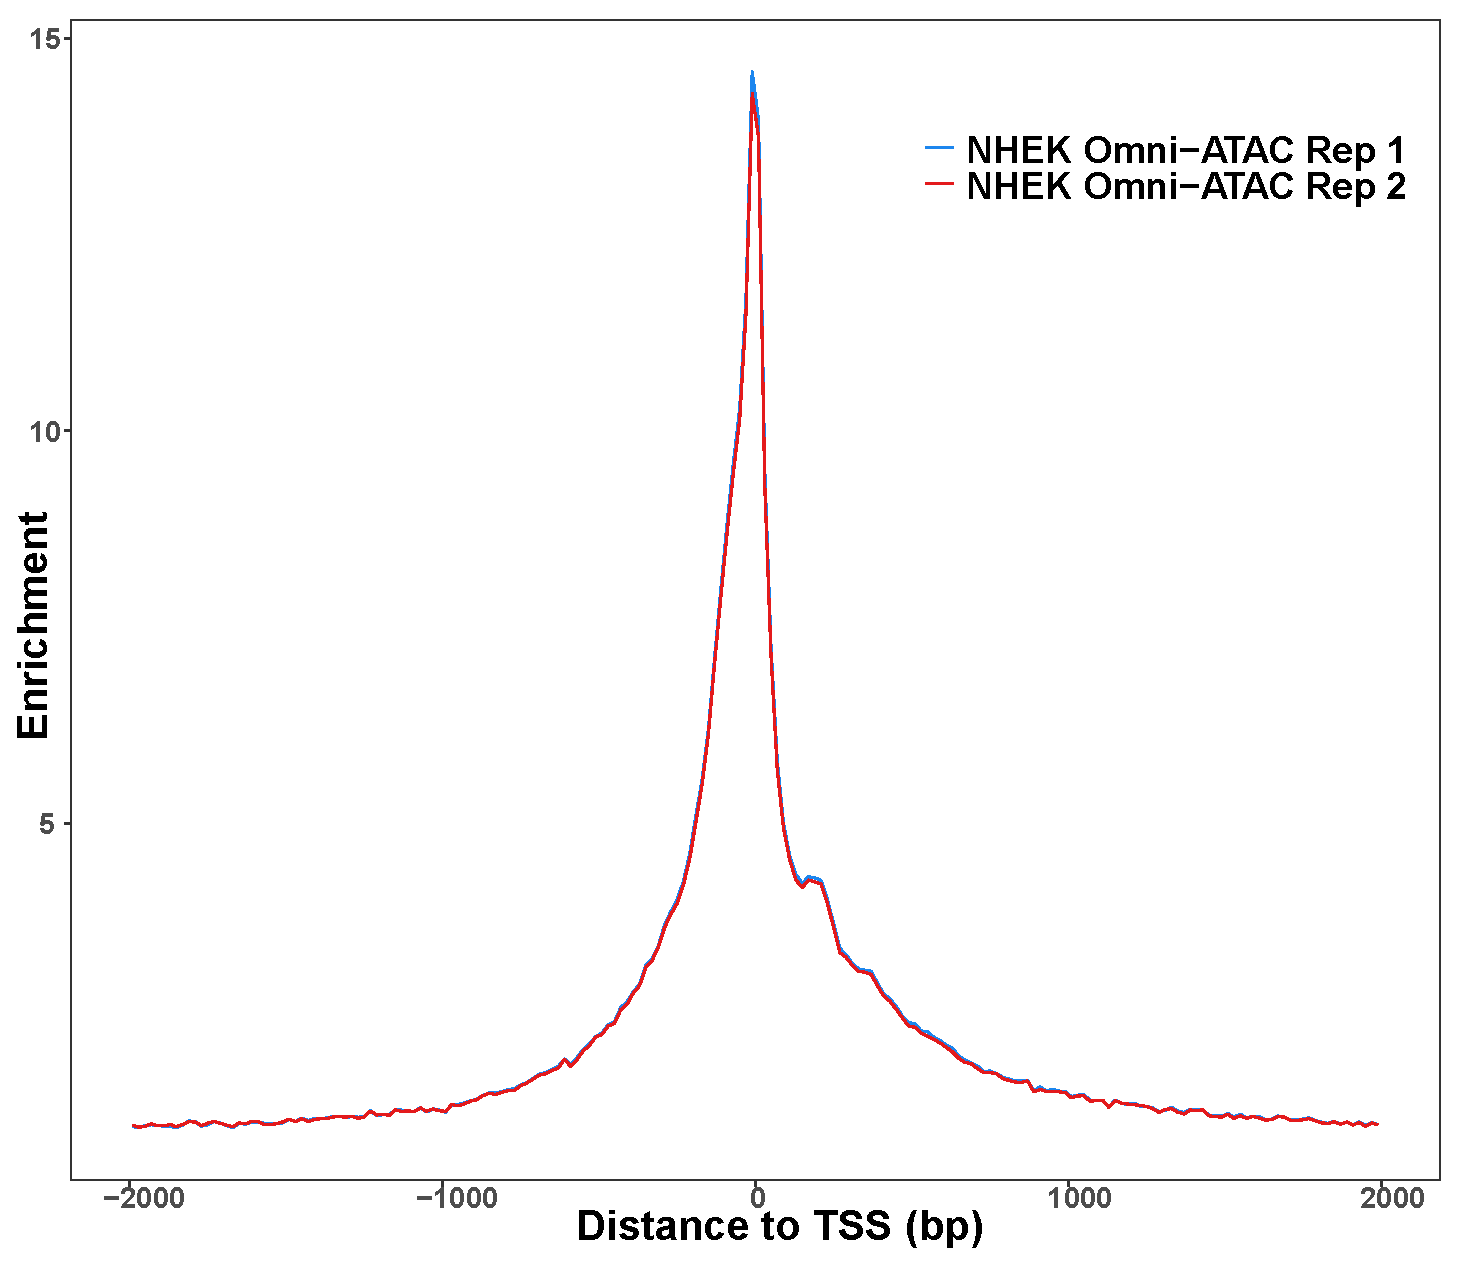
\includegraphics[width=\textwidth]{./Results1/pdfs/ATAC_skin_TSS_enrichment_NHEK_omni_ATAC}
\caption{\textbf{}} % to add text to the figure name
\end{subfigure}%
\caption[QC assessment of FAST-ATAC and Omni-ATAC in cultured NHEK]{\textbf{QC assessment of FAST-ATAC and Omni-ATAC in cultured NHEK.\\
}}
\label{fig:PS02_skin_ATAC_QC_assessment}
\end{figure} 






Omni-ATAC
Tapestation profiles of the the chosen condition include it with the supplementary that includes all other tapestation profiles.done
QC measurements: frag size distribution and TSS done
Track including all skin samples

Think of what to include about the biopsies in supplementary done



\begin{figure}[htbp]
\centering
\begin{subfigure}{0.5\textwidth}
\centering
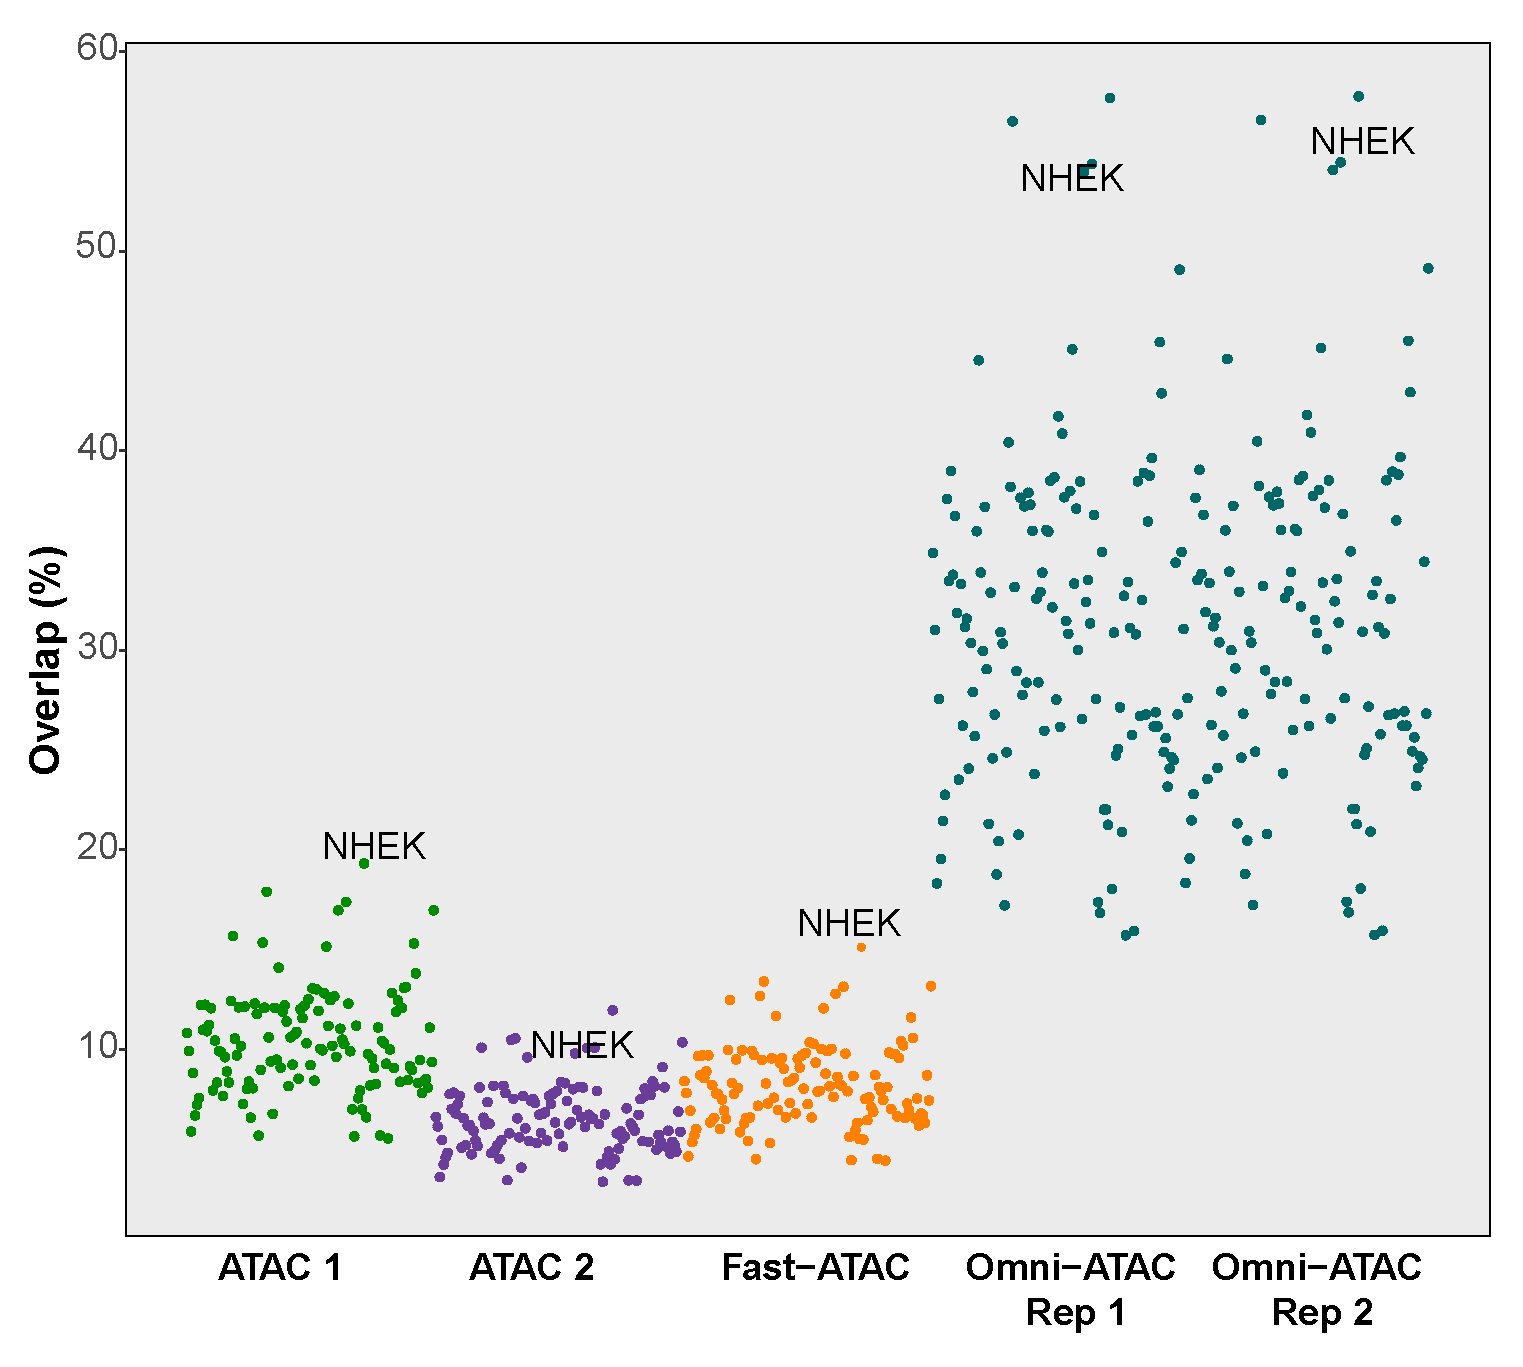
\includegraphics[width=\textwidth]{./Results1/pdfs/ENCODE_125_cell_types_overlap_FAST_ATAC_Omni_ATAC_pval_2}
\caption{\textbf{}}
% The percentage sign indicated that the other subfig goes side by side
\end{subfigure}%
\begin{subfigure}{0.5\textwidth}
\centering
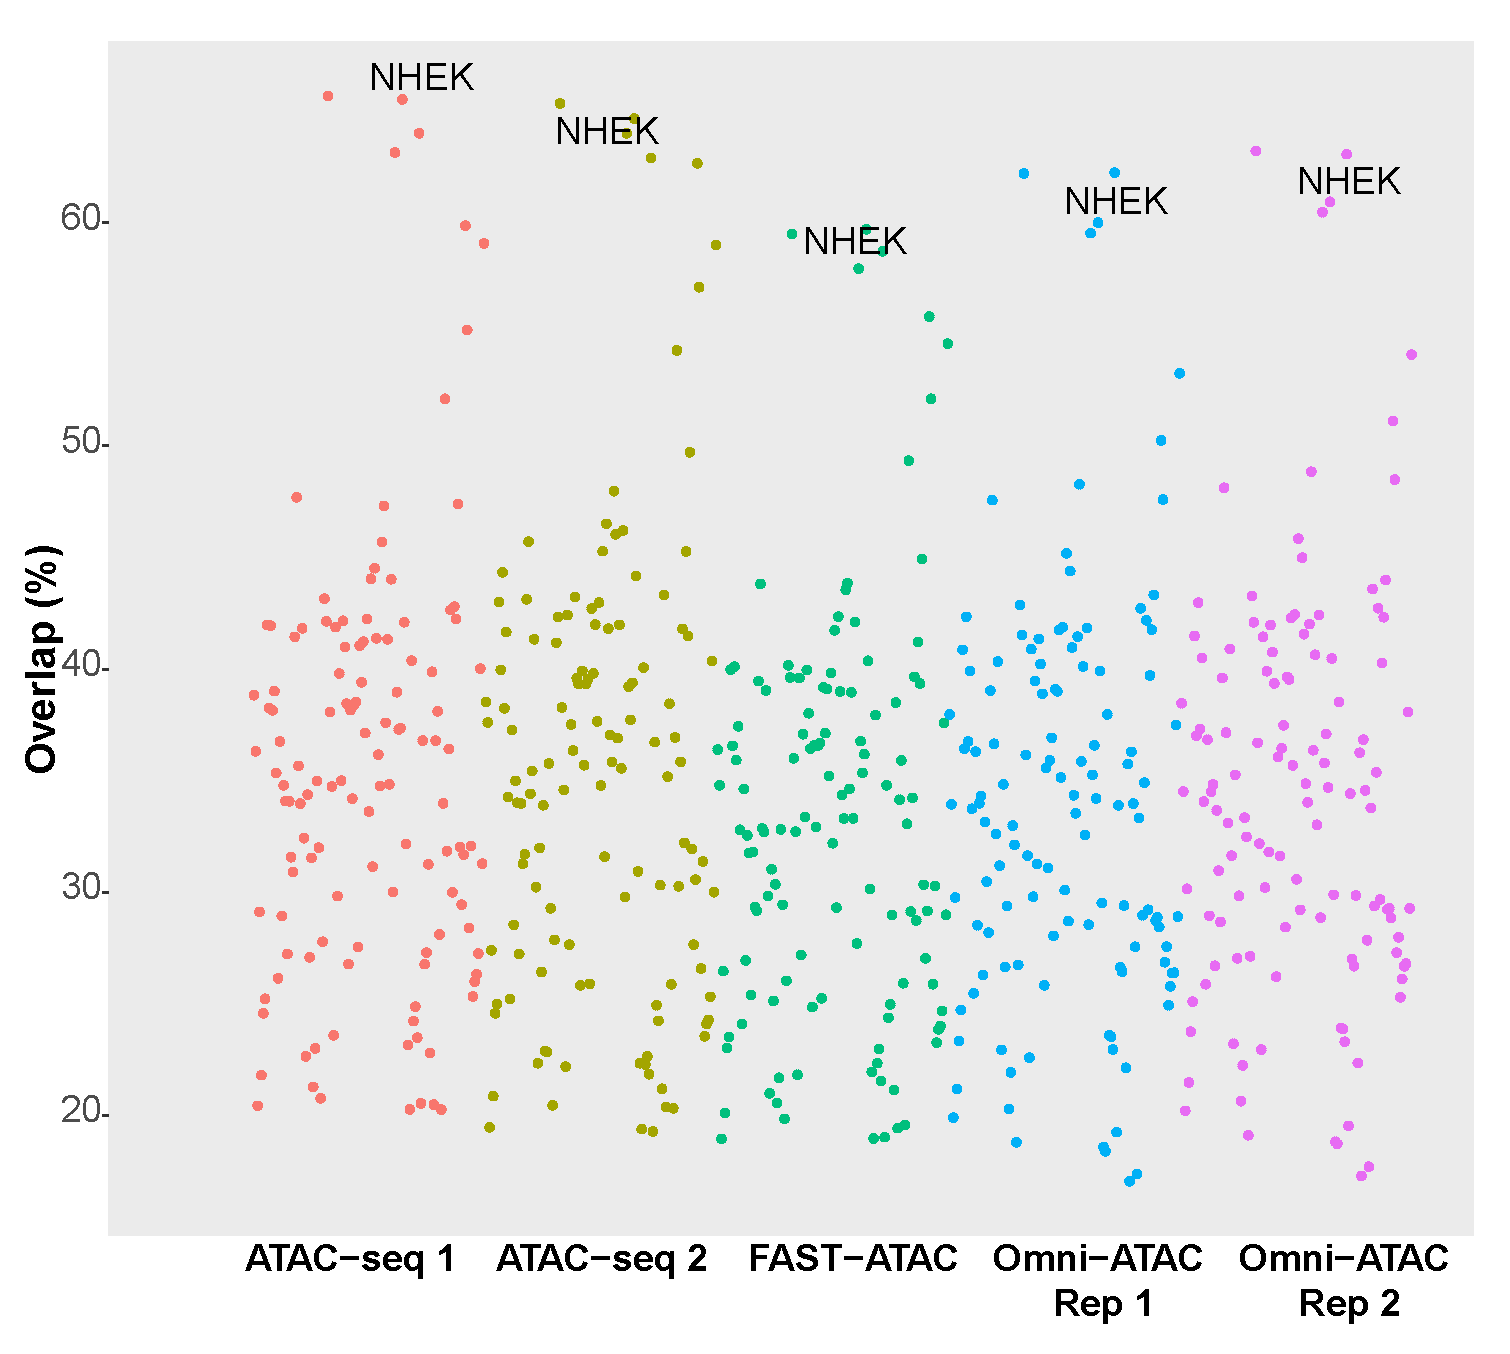
\includegraphics[width=\textwidth]{./Results1/pdfs/ENCODE_125_cell_types_overlap_FAST_ATAC_Omni_ATAC_qval_2}
\caption{\textbf{}}
\end{subfigure}
\begin{subfigure}{0.5\textwidth}
\centering
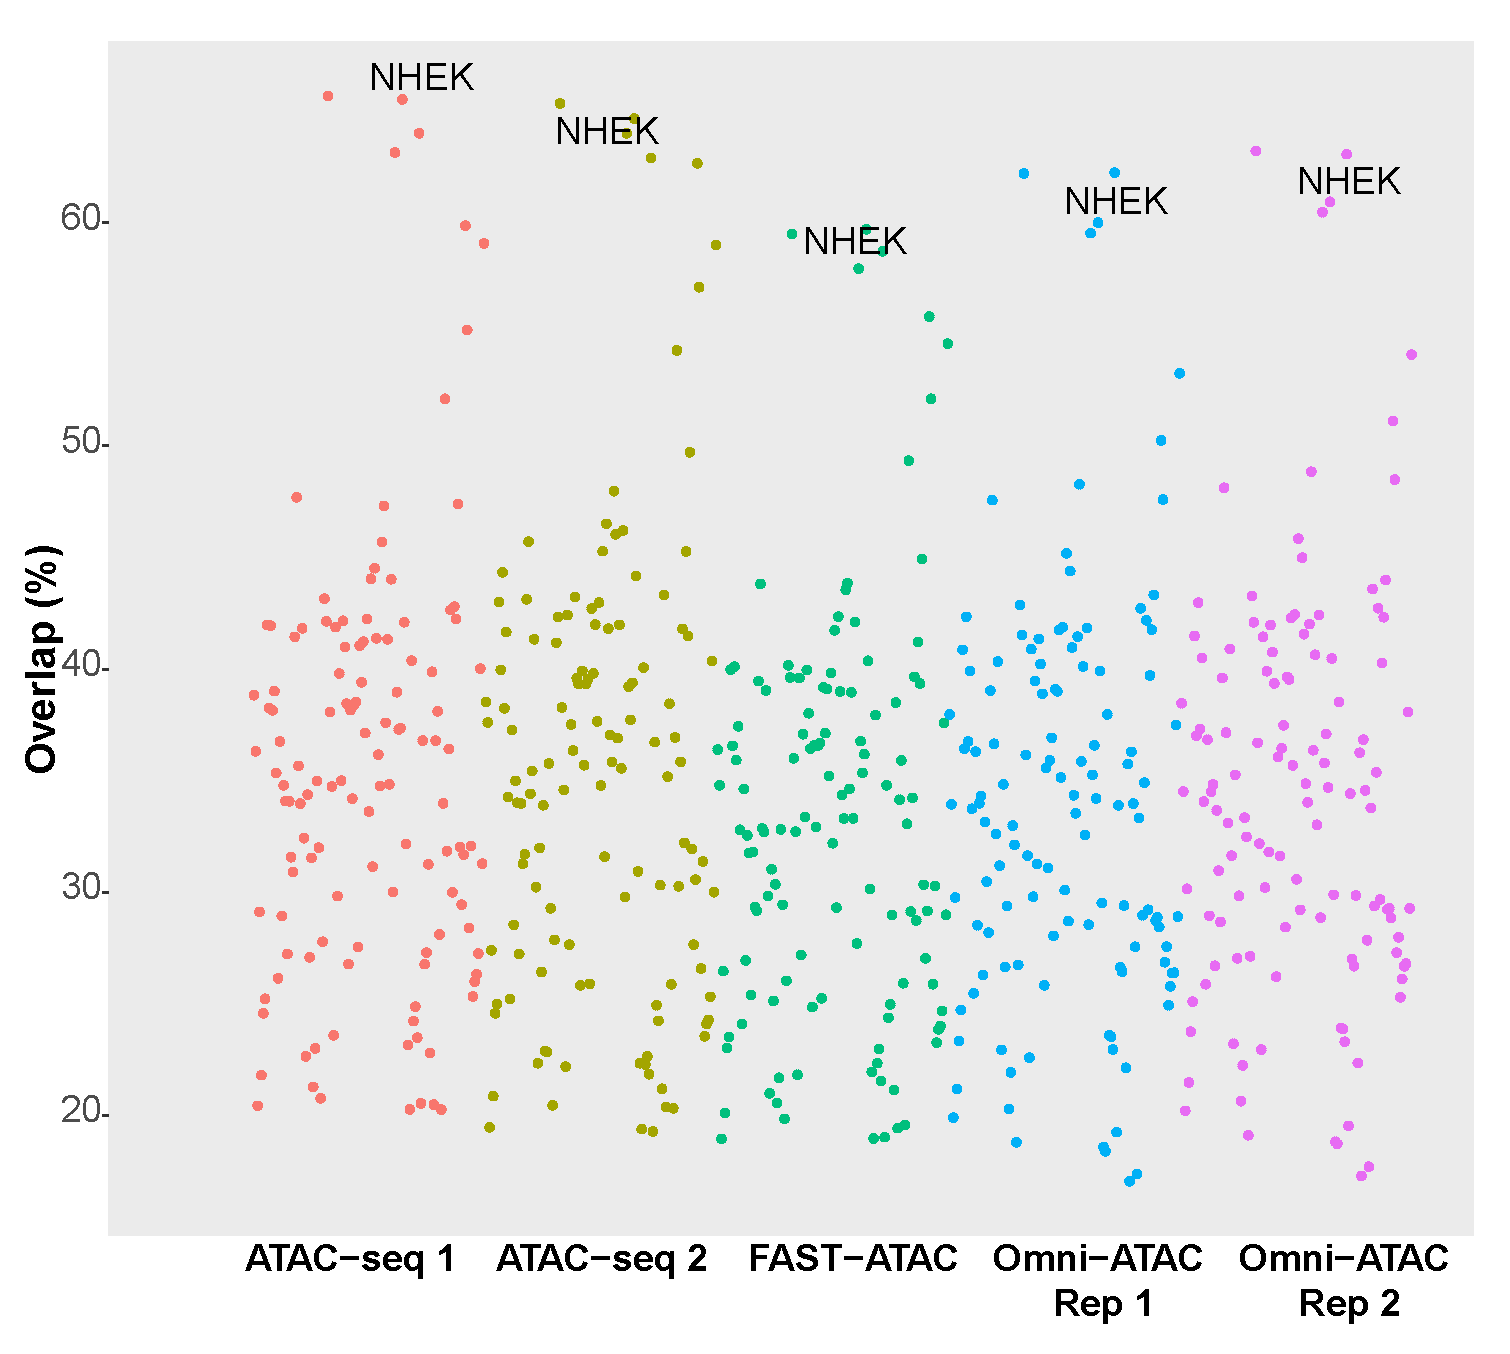
\includegraphics[width=\textwidth]{./Results1/pdfs/ENCODE_125_cell_types_overlap_FAST_ATAC_Omni_ATAC_qval_2}
\caption{\textbf{}} % to add text to the figure name
\end{subfigure}%
\caption[QC assessment of Omni-ATAC in NHEK and chromatin accessibility signal for the samples generated with the different ATAC-seq protocols]{\textbf{QC assessment of Omni-ATAC in NHEK and chromatin accessibility signal for the samples generated with the different ATAC-seq protocols}.\\}
\label{fig:Omni_ATAC_NHEK_QC_assessment_and_all_tracks}
\end{figure} 



\subsection{Discussion}
Maybe justify in the dicussion the use of DESEq2 and limma shared based on Alasoo observation of noise effect in limma